\documentclass[hidelinks]{ipn}
\usepackage{ipnstyle}
\usepackage{lipsum}
\usepackage{graphicx}
\usepackage{float}
\usepackage{caption}
\usepackage{subcaption}
\usepackage{bookmark}
\usepackage{hyperref}
\usepackage{minted}
% \usepackage{cite}

\usepackage{tikz, lipsum, lmodern}
\usepackage[most]{tcolorbox}
\usepackage{etoolbox}  % Añade esta línea
\usepackage{microtype}  % Mejora la justificación y tipografía
\usepackage{ragged2e}  % Añade esta línea en el preámbulo
\usepackage{parskip}
\usepackage{changepage} % en el preámbulo
\usepackage{bm}      % For bold math symbols (\bm command)
\usepackage{array}   % For better table column specifications
\usepackage{longtable}
\usepackage{booktabs}% For professional looking tables (\toprule, \midrule, \bottomrule)
\usepackage{adjustbox}
\usepackage{enumitem}
\usepackage{pgffor}
\usepackage{enumitem}
\usepackage{pdflscape}  % para PDF

% Tikz packages
\usetikzlibrary{shapes, arrows, positioning, calc}

% enlistar con mayor profundidad
\setlist[itemize,1]{label=\textbullet,ref={}}
\setlist[enumerate,1]{label=\arabic*.}
\setlistdepth{15}

\setlength{\parindent}{0pt}
% Añade esta línea antes de \begin{document}
\let\cleardoublepage\clearpage
\setlength{\emergencystretch}{3em}
\tolerance=9999
\AtBeginDocument{\justifying}

\makeatletter
\makeatother

\author{José Emiliano Carrillo Barreiro\\
        José Ángel Robles Otero}
\title{Modelo para representar comportamientos gravitacionales con dos cuerpos}
\schoolname{Escuela Superior de Cómputo}
\degree{Maestría en Ciencias de la Computación}
\advisor{Dr.\ Cesar Hernández Vasquez}
\coadvisor{Dr.\ Mauricio Olguín Carbajal}
\academicyear{\today}

\hypersetup{
    colorlinks=false,
    pdfauthor={Your Name},
    pdftitle={Modelo para representar comportamientos gravitacionales con dos cuerpos},
    pdfsubject={Thesis},
    pdfkeywords={keyword1, keyword2, keyword3}
    pdfproducer={Latex with hyperref},
    pdfcreator={pdflatex}
}

\addbibresource{./references.bib}
\pagestyle{headings}

\newcommand{\vect}[1]{\mathbf{#1}}

\begin{document}
\justifying%
\frontmatter
    \maketitle
    \begin{titlepage}
    \begin{center}
        % Logo and Institute Name placement
        \raisebox{0.0\height}{
        \begin{adjustbox}{max width=1.2\linewidth, right}
          \begin{minipage}[c]{0.5\linewidth}
            \centering
           \raisebox{0.0\height}{
\includegraphics[width=0.5\linewidth]{img/logo-ipn.png}}
          \end{minipage}\hfill
          \begin{minipage}[c]{1.5\linewidth}
            \centering
            {\fontsize{28}{30}\selectfont\textsc{Instituto Politécnico Nacional}}\\[2mm]
            {\fontsize{24}{26}\selectfont\textsc{Escuela Superior de Cómputo}}\\[2mm]
            {\fontsize{20}{22}\selectfont\textsc{Subdirección Académica}}
        \end{minipage}
        \hfill
          \begin{minipage}[c]{0.5\linewidth}
            \centering
            \raisebox{0.0\height}{
\includegraphics[width=0.8\linewidth]{img/EscudoESCOM.png}}
          \end{minipage}
        \end{adjustbox}}

        \begin{adjustwidth}{-2.5cm}{}
            \begin{center}
                \begin{tabular}{c@{\hspace{8cm}}c}
                    No.\ de TT:\ 2025-B065 &
                    \today
                \end{tabular}\\
                \vspace{0.55cm}
                \textbf{Documento técnico} \\
                
                \vspace{0.5cm}
                
                % Title
                \begin{minipage}{0.8\textwidth}
                    \centering
                    {\fontsize{16}{16}\selectfont\textbf{``Modelo para representar comportamientos gravitacionales con dos cuerpos''\\}}
                \end{minipage}
                
                \vspace{0.3cm}
                
                % Presentan
                {\fontsize{16}{16}\selectfont\textit{Presentan:}} \\
                \vspace{0.25cm}
                % Authors (names in alphabetical order by last name)
                {\fontsize{14}{14}\selectfont\textbf{
                José Emiliano Carrillo Barreiro.\footnote{\href{mailto:carrillobarjosee@gmail.com}{carrillobarjosee@gmail.com}}\\
                José Ángel Robles Otero.\footnote{\href{mailto:robles.otero.jose.angel@gmail.com}{robles.otero.jose.angel@gmail.com}}}
                }
                \vspace{0.5cm}
                
                % Directors
                {\fontsize{14}{14}\selectfont\textsc{Directores:\\}}
                
                \vspace{10pt}
                
                % Director names
                {\fontsize{14}{14}\selectfont\textbf{Dr.\ Cesar Hernández Vasquez\\}}
                
                \vspace{5pt}
                
                % Co-director (if applicable)
                {\fontsize{14}{14}\selectfont\textbf{Dr.\ Mauricio Olguín Carbajal}}
                
                \vspace{0.5cm}
                
                % Abstract
                \begin{minipage}{\textwidth}
                    \begin{center}
                        \textbf{Resumen:}\\[0.3cm]
                    \end{center}
                    {\fontsize{12}{12}\selectfont
                    En los últimos años, la elaboración de entornos virtuales complejos, como \textit{REBOUND}, \textit{Universe sandbox}, \textit{Stellarium} y \textit{Celestia}, han experimentado un crecimiento exponencial en sus capacidades. Más, cuando se habla de implementar mejoras en la precisión y escalabilidad dentro de sistemas de \textit{n}-cuerpos celestes, por ejemplo, la simulación de nacimientos de galaxias, todavía existen dificultades, ya que, actualmente, los modelos que los simulan no permiten introducir cambios en los parámetros de los cuerpos durante su ejecución, parámetros como la velocidad, posición y masa del cuerpo, lo que impide contar con escenarios más fidedignos a los comportamientos  físicos dentro de sistemas de $n$-cuerpos atípicos. En este proyecto, se propone solucionar este problema mediante la construcción de un modelo que permita realizar cambios al parámetro más significativo del  sistema, compuesto por dos cuerpos, en tiempo de ejecución, implementando técnicas como el método multipolar rápido (FMM, por sus siglas en inglés, \textit{Fast Multipole Method}), el \textit{algoritmo de Barnes-Hut} y algoritmos bioinspirados. La solución que se desarrolle podría usarse para simular comportamientos físicos dentro de entornos virtuales.\\

                     \textbf{Palabras clave: } Modelado y Simulación de sistemas, problema de los $n$-cuerpos, Mecánica Celeste, y Algoritmos Bioinspirados.}
                \end{minipage}
                
                \vspace{0.7cm}
                
                % Date
                \textbf{\large Fecha: \today}
            \end{center}
        \end{adjustwidth}
    \end{center}
\end{titlepage}
    \filright
\begin{minipage}{\textwidth}
    \filright
    \centering
    \begin{tcolorbox}[enhanced,attach boxed title to top center={yshift=-3mm,yshifttext=-1mm},
      colback=blue!5!white,colframe=blue!75!black,colbacktitle=red!80!black,
      title=\textbf{Advertencia},fonttitle=\bfseries,
      boxed title style={size=small,colframe=red!50!black} ]
    \textit{“Este documento contiene información desarrollada por la Escuela
    Superior de Cómputo del Instituto Politécnico Nacional, a partir de datos y
    documentos con derecho de propiedad y por lo tanto, su uso quedará
    restringido a las aplicaciones que explícitamente se convengan.”}\\
    
    La aplicación no convenida exime a la escuela su responsabilidad técnica y
    da lugar a las consecuencias legales que para tal efecto se determinen.\\
    
    Información adicional sobre este reporte técnico podrá obtenerse en:\\
    
    La Subdirección Académica de la Escuela Superior de Cómputo del Instituto
    Politécnico Nacional, situada en Av. Juan de Dios Bátiz s/n Teléfono: 57296000, extensión 52000.
    \end{tcolorbox}
\end{minipage}
    \input{frontmatter/00-Advertencia}
    \chapter{Resumen.}
\justifying
En los últimos años, la elaboración de entornos virtuales complejos, 
como \textit{REBOUND}, \textit{Universe sandbox}, \textit{Stellarium} y \textit{Celestia}, 
han experimentado un crecimiento exponencial en sus capacidades. Más, cuando se habla de 
implementar mejoras en la precisión y escalabilidad dentro de sistemas de \textit{n}-cuerpos celestes, 
por ejemplo, la simulación de nacimientos de galaxias, todavía existen dificultades, ya que, actualmente, 
los modelos que los simulan no permiten introducir cambios en los parámetros de los cuerpos durante su ejecución, 
parámetros como la velocidad, posición y masa del cuerpo, lo que impide contar con escenarios más fidedignos a los 
comportamientos  físicos dentro de sistemas de $n$-cuerpos atípicos. En este proyecto, se propone solucionar este 
problema mediante la construcción de un modelo que permita realizar cambios al parámetro más significativo del  sistema, 
compuesto por dos cuerpos, en tiempo de ejecución, implementando técnicas como el método multipolar rápido (FMM, por sus siglas en inglés, 
\textit{Fast Multipole Method}), el \textit{algoritmo de Barnes-Hut} y algoritmos bioinspirados. La solución que se desarrolle podría usarse 
para simular comportamientos físicos dentro de entornos virtuales.\\

\chapter{Abstract.}
\lipsum[1-3]
    \chapter{Agradecimientos.}
El presente trabajo terminal, documentado en este informe técnico, no habría sido posible sin el invaluable apoyo, la guía y la inspiración de numerosas personas a lo largo de nuestra trayectoria académica. A todos ellos, expresamos nuestro más profundo y sincero agradecimiento.

En primer lugar, deseamos reconocer a nuestros directores, el Dr.\ Cesar Hernández Vásquez y el Dr.\ Mauricio Olguín Carbajal, por su dedicación, paciencia y valioso apoyo intelectual durante este proceso. Su orientación especializada, sus críticas constructivas y su constante motivación han sido pilares fundamentales en el desarrollo de la investigación y la propuesta de solución planteada en este proyecto. Sin su confianza y disposición para compartir su conocimiento, esta primera presentación de resultados no habría alcanzado su forma actual.

Asimismo, extendemos nuestra gratitud a los miembros del comité sinodal, la Dra. Yesica Sonia Flores Meraz, el M. en C. Jesús Alfredo Martínez Nuño y el Dr.\ Genaro Juárez Martínez, por su tiempo, esfuerzo y compromiso al evaluar este trabajo terminal. Sus comentarios y sugerencias han enriquecido significativamente la calidad de esta investigación y seguirán siendo esenciales para su mejora.

De manera especial, agradecemos a la Dra. Lorena Chavarría Báez por su apoyo incondicional en el planteamiento del protocolo y la delimitación del proyecto. Sus aportaciones y sugerencias fueron cruciales para afinar el enfoque de esta investigación, contribuyendo a la profundidad y claridad que caracterizan el trabajo aquí presentado.

Igualmente, queremos destacar la colaboración de los Dr.\ Daniel Molina Pérez y M. en C. José Alberto Torres León, quienes, en su rol de consultores expertos, revisaron el propósito, los objetivos y el desarrollo de este proyecto. Su retroalimentación, validada mediante el “juicio de experto”, junto con sus valiosos comentarios, nos permitió perfeccionar las técnicas y la calidad de este informe.

Por último, pero no menos importante, rendimos homenaje a nuestras familias por su amor incondicional, paciencia y sacrificios a lo largo de este arduo camino. Su respaldo constante ha dado un significado especial a esta presentación.
A través de esta primera parte del trabajo terminal, hemos enfrentado desafíos que nos han permitido crecer tanto personal como académicamente. Este proceso nos ha revelado nuevas dimensiones del conocimiento, así como la resiliencia y determinación que habitan en nosotros. A todos quienes nos han acompañado con su apoyo, guía e inspiración, les debemos una parte esencial de este logro inicial. Gracias por todo.

    \tableofcontents
    \listoffigures
    \listoftables
    \listofalgorithms%

\mainmatter%
    %\chapter{Introduction}\label{ch:Introduction}
Incluir una breve introducción al proyecto, incluyendo antecedentes, un poco de historia, de dónde surge el proyecto, qué motivó a la realización del proyecto. NO incluir la problemática ni la solución, ni justificación. [Mínimo media cuartilla, máximo una y media]
\section{Research problem}
\lipsum[1]
\begin{definition}[Open space]
A subset $U$ of a metric space $(M, d)$ is called open if, for any point $x$ in $U$, there exists a real number $\epsilon > 0$ such that any point $y\in M$ satisfying $d(x, y) < \epsilon$ belongs to $U$. Equivalently, $U$ is open if every point in $U$ has a neighborhood contained in $U$.
\end{definition}
\lipsum[1]

\section{Objectives}
\subsection{General objective}
Lorem ipsum dolor sit amet, consectetuer adipiscing elit~\cite{adam2015higgs, atlas2014neural, baldi2014searching}. Ut purus elit, vestibulum ut, placerat ac, adipiscing vitae, felis. Curabitur dictum gravida mauris. Nam arcu libero, nonummy eget, consectetuer id, vulputate a, magna.

\subsection{Specific objectives}
Lorem ipsum dolor sit amet, consectetuer adipiscing elit:
\begin{itemize}
    \item Lorem ipsum dolor sit amet, consectetuer adipiscing elit. Ut purus elit, vestibulum ut, placerat ac, adipiscing vitae, felis. Curabitur dictum gravida mauris.
    \item Nam arcu libero, nonummy eget, consectetuer id, vulputate a, magna.
    \item  Pellentesque habitant morbi tristique senectus et netuset malesuada fames ac turpis egesta
\end{itemize}

\section{Justification}
\lipsum[1]

\section{Project scope and limitations}
\lipsum[1]
\begin{theorem}
The kernel of a linear transformation from a vector space V to a vector space W is a subspace of V.
\end{theorem}
\begin{proof}
    Suppose that u and v are vectors in the kernel of L.  Then 
    \begin{equation}
        L(u) = L(v) = 0
    \end{equation}
    We have
    \begin{equation}
        L(u + v) = L(u) + (v) = 0 + 0 = 0 
    \end{equation}
    and
    \begin{equation}
        L(cu) = cL(u) = c0 = 0
    \end{equation}
    Hence $u + v$ and cu are in the kernel of $L$. We can conclude that the kernel of $L$ is a subspace of $V$.
\end{proof}
\lipsum[1]

\begin{algorithm}[H]
    \caption{Descenso de gradiente estocástico}\label{alg:SGD}
    \hspace*{\algorithmicindent} \textbf{parameters} \\
    \hspace*{\algorithmicindent}\hspace*{\algorithmicindent} Número de iteraciones $\tau$ \\
    \hspace*{\algorithmicindent}\hspace*{\algorithmicindent} Tasa de aprendizaje $\eta$ \\
    \hspace*{\algorithmicindent}\hspace*{\algorithmicindent} Parámetro de regularización $\lambda$ \\
    \hspace*{\algorithmicindent} \textbf{input} \\
    \hspace*{\algorithmicindent}\hspace*{\algorithmicindent} Pesos iniciales $\mathbf{w}^{(1)}$ \\
    \hspace*{\algorithmicindent}\hspace*{\algorithmicindent} Gradiente en una muestra $\mathcal{Q}_i(w)$
    \begin{algorithmic}[1]
        \Procedure{SGD}{$\mathbf{w}^{(1)}, \sigma$}
        \For{$i \gets 1, 2, \dots, \tau$}
        \State Selecciona una muestra $(\mathbf{x}, \mathbf{y})\sim D$
        \State Calcula el gradiente $\nabla\mathcal{Q}_i(w)$ para la muestra $(\mathbf{x}, \mathbf{y})$
        \State Asigna $\mathbf{w}^{(i+1)} \gets \mathbf{w}^{(i)} - \eta(\nabla\mathcal{Q}_i(w) + \lambda\mathbf{w}^{(i)})$
        \EndFor
        \EndProcedure
    \end{algorithmic}
\end{algorithm}

\section{Hypothesis}
\lipsum[1-2]

\section{Project organization}
\lipsum[1-2]
    %\chapter{Conclusions}\label{ch:Conclusions}
\lipsum[1]
\begin{table}[hbtp]
    \centering
    \begin{tabular}{@{}*{2}{p{0.5\textwidth}}@{}}
        \toprule
        \textbf{Correct} &  \textbf{Incorrect}
        \\
        \midrule
        \enquote{This is an \enquote{inner quote} inside an outer quote}
        &
        "This is an 'inner quote' inside an outer quote"
        \\
        \bottomrule
    \end{tabular}
    \caption[Quotation marks]
    {Proper quotation mark usage.
    The \texttt{\textbackslash enquote} command chooses the correct
    quotation marks for the specified language.}
\end{table}
\lipsum[1]

\section{Recommendations and future work}
\lipsum[1]
    \chapter{Introducción}\label{ch:Introducción}
    \section{Antecedentes}
El desarrollo de simulaciones de \textit{n}-cuerpos ha sido ampliamente investigado con el objetivo de mejorar su capacidad para modelar fenómenos complejos en entornos como la colisión de galaxias y la evolución de sistemas planetarios. Sin embargo, una limitación crítica es la incapacidad de ajustar los parámetros de los cuerpos durante la ejecución de la simulación, lo que afecta la representación precisa de eventos masivos como colisiones en las simulaciones disponibles.

El problema de los \textit{n}-cuerpos\footnote{El problema de \textit{n}-cuerpos se refiere al estudio del movimiento e interacción gravitacional de varios cuerpos bajo sus influencias mutuas. En la sección \ref{sec:n-body_problem} se profundiza a fondo el termino.} ha sido uno de los desafíos más complejos en la mecánica celeste, desde los trabajos pioneros de Newton en el siglo XVII. Si bien el problema de los dos cuerpos tiene una solución analítica exacta bajo ciertas condiciones, cuando se introducen factores adicionales, se requieren métodos numéricos avanzados para mejorar la precisión de las simulaciones.

Avances como el método multipolar rápido (FMM, por sus siglas en inglés, \textit{Fast Multipole Method})\footnote{El FMM es un algoritmo que optimiza el cálculo de interacciones entre partículas distantes en sistemas físicos, como los gravitacionales, agrupando partículas y aproximando su influencia colectiva, lo que reduce la complejidad computacional de \(O(n^2)\) a \(O(n)\) o \(O(n \log n)\).} y el algoritmo de Barnes-Hut\footnote{El algoritmo de Barnes-Hut es una técnica de simulación de \textit{n}-cuerpos que aproxima las fuerzas gravitacionales al agrupar cuerpos distantes en una misma región del espacio, representándolos como una única masa, lo que reduce la complejidad computacional de \(O(n^2)\) a \(O(n \log n)\).} han optimizado las simulaciones de \textit{n}-cuerpos al reducir la complejidad computacional en el cálculo de las interacciones gravitacionales. Sin embargo, la falta de capacidad para ajustar dinámicamente las propiedades de los cuerpos durante la ejecución sigue siendo una limitación en la representación realista de eventos astronómicos.

Estudios recientes han introducido herramientas y enfoques que podrían mejorar las simulaciones de \textit{n}-cuerpos, como el uso de árboles cuádruples y octales para la representación geométrica y la aplicación de inteligencia artificial en las simulaciones moleculares que podrían inspirar nuevas técnicas en simulaciones celestes. Además, se ha demostrado la eficacia de integradores simplécticos\footnote{Los integradores simplécticos son métodos numéricos utilizados para resolver ecuaciones diferenciales en sistemas dinámicos conservando las propiedades geométricas del sistema, como la conservación de la energía a largo plazo, lo que los hace especialmente adecuados para simular interacciones físicas, como las gravitacionales, en sistemas de \textit{n}-cuerpos.} para garantizar la estabilidad de las simulaciones durante colisiones y la paralelización para mejorar la eficiencia en simulaciones masivas.
    \section{Planteamiento del problema}
Las simulaciones de sistemas de \textit{n}-cuerpos celestes han sido una herramienta fundamental en la astronomía y la mecánica celeste para estudiar la evolución de sistemas planetarios, la dinámica estelar y la interacción gravitacional a gran escala. Sin embargo, una limitación crítica en los modelos actuales es la imposibilidad de modificar dinámicamente los parámetros de los cuerpos durante la ejecución de la simulación. En la mayoría de los simuladores, estos parámetros, como la masa, la energía del sistema, la posición y el tiempo de existencia de los cuerpos se definen antes de la ejecución, impidiendo la representación precisa de eventos atípicos o transitorios, como colisiones de galaxias, acreción de materia en discos protoplanetarios o cambios de masa en estrellas variables.

Uno de los problemas más importantes derivados de esta limitación es la incapacidad de ajustar la masa de los cuerpos celestes durante el lapso de duración de la simulación. En eventos como fusiones de agujeros negros o estrellas en procesos de acreción, la masa de los cuerpos cambia significativamente a lo largo del tiempo, alterando la evolución del sistema. Sin la posibilidad de modificar este parámetro de manera dinámica, los modelos actuales ofrecen solo aproximaciones estáticas que no reflejan con precisión la naturaleza de estos fenómenos.

Además, el rendimiento computacional también representa un desafío. La simulación de \textit{n}-cuerpos es un problema computacionalmente costoso, ya que la cantidad de interacciones a calcular crece cuadráticamente con el número de cuerpos ($O~(n^2)$), lo que hace que las simulaciones a gran escala sean prohibitivas en términos de tiempo de ejecución y recursos computacionales. Métodos como el algoritmo de Barnes-Hut y el método multipolar rápido han sido desarrollados para mitigar este problema reduciendo la cantidad de cálculos directos, pero no abordan la falta de flexibilidad en la modificación de parámetros en tiempo real.

En este contexto, la incapacidad de modificar parámetros dinámicamente en simulaciones de \textit{n}-cuerpos afecta no solo a la estabilidad del sistema representado durante la simulación, respecto a los fenómenos astronómicos internos del sistema; sino también la capacidad de realizar simulaciones interactivas, algo que podría tener aplicaciones en la enseñanza, la exploración espacial y la industria del entretenimiento. La ausencia de modelos que permitan esta flexibilidad limita el alcance de las simulaciones actuales y plantea la necesidad de desarrollar enfoques más adaptativos y eficientes.
    \section{Propuesta de solución}

La solución propuesta se basa en el desarrollo de un modelo que permite la modificación dinámica de parámetros durante la simulación, lo que representa una mejora significativa con respecto a los simuladores tradicionales, que requieren reconfiguraciones antes de cada ejecución. Este modelo integrará técnicas avanzadas para optimizar el cálculo de interacciones gravitacionales y garantizar la estabilidad de la simulación.

Para lograrlo, se empleará el método multipolar rápido (FMM) y el algoritmo de Barnes-Hut, ambos ampliamente utilizados para reducir la complejidad computacional en simulaciones de \textit{n}-cuerpos sin comprometer la precisión . Estas técnicas permiten agrupar cuerpos en estructuras jerárquicas, disminuyendo el número de cálculos directos y mejorando la eficiencia del sistema.

Además, la implementación de algoritmos bioinspirados, como la optimización por enjambre de partículas (PSO) y algoritmos genéticos, permitirá el ajuste dinámico de los parámetros de los cuerpos celestes, garantizando un comportamiento estable incluso en escenarios de colisión o interacciones complejas. Estas estrategias facilitarán la identificación y ajuste de valores óptimos sin necesidad de intervención manual, lo que hará que la simulación sea más adaptable a eventos inesperados.

El modelo se diseñará para ser escalable, permitiendo la modificación en tiempo real de los parámetros de hasta dos cuerpos celestes, con la posibilidad de extenderse a más cuerpos en implementaciones futuras. Su integración con entornos virtuales como Unreal Engine o motores de simulación especializados permitirá su aplicación en campos como la educación, los videojuegos y la industria aeroespacial.

Para garantizar un rendimiento eficiente, el modelo se desarrollará optimizado para ejecutarse en hardware de gama media, como procesadores multinúcleo con al menos 16 GB de RAM. Esto asegurará que la solución sea accesible sin requerir infraestructuras de alto rendimiento, ampliando su potencial uso en distintos ámbitos.

Esta combinación de técnicas avanzadas y adaptabilidad en tiempo real establece una base innovadora para el desarrollo de simulaciones gravitacionales más dinámicas, eficientes y versátiles, superando las limitaciones de los modelos preconfigurados actuales.
    \section{Objetivo general}
Desarrollar un modelo teórico para la simulación del problema de dos cuerpos que permita la modificación dinámica de la masa, mejorando la estabilidad local del sistema visible en la representación de sus interacciones gravitacionales y eventos asociados.
\subsection{Objetivos específicos}
\begin{itemize}
    \item Implementar el módulo de simulación encargado de integrar los distintos procedimientos algorítmicos requeridos para obtener la descripción numérica del sistema de interacción de n cuerpos, incluyendo la aplicación de métodos de integración numérica, el cálculo de fuerzas gravitatorias y la detección de colisiones.

    \item Diseñar e implementar el módulo de optimización orientado al ajuste dinámico de las masas de los cuerpos que conforman el sistema de \textit{n}-cuerpos, mediante el uso de algoritmos bioinspirados, con el fin de identificar el primer conjunto de valores que satisfaga las restricciones impuestas en cuanto a estabilidad y viabilidad del sistema.

    \item Desarrollar e implementar el modelo computacional de para la simulación dinámica de un sistema de dos cuerpos bajo interacción gravitatoria.

    \item Implementar el módulo de visualización gráfica para la representación dinámica del sistema simulado, mostrando su evolución temporal a lo largo de un conjunto limitado de iteraciones, a fin de apoyar la interpretación de los resultados del modelo

    \item Diseñar e implementar una interfaz básica que permita el ingreso estructurado de parámetros asociados a los cuerpos del sistema, diferenciando entre atributos fijos (e.g., radio) y variables susceptibles de optimización (e.g., masa), así como la definición de restricciones obligatorias y opcionales que condicionan el espacio de soluciones. Además de permitir visualizar los resultados generados por los módulos de simulación y optimización
\end{itemize}
    \section{Justificaión}
Este proyecto es relevante porque introduce un enfoque innovador en la simulación de sistemas gravitacionales al permitir la modificación dinámica de parámetros, superando las limitaciones de los modelos tradicionales. La elección de algoritmos avanzados, como el método multipolar rápido (FMM) y el algoritmo de Barnes-Hut, garantiza un equilibrio entre precisión y eficiencia computacional, lo que permite su aplicación en escenarios más complejos sin un costo computacional excesivo. Además, la implementación de técnicas de optimización bioinspiradas ofrece un método adaptable para ajustar el sistema en tiempo real, mejorando la fidelidad de las simulaciones.

El uso de estas tecnologías no solo optimiza el rendimiento de la simulación, sino que también sienta las bases para su posible escalabilidad a problemas de mayor complejidad, como la simulación de múltiples cuerpos. Aunque el presente trabajo se centra en el problema de dos cuerpos, su enfoque y metodología podrían aplicarse en otros ámbitos, como el modelado de interacciones gravitacionales en videojuegos y simulaciones interactivas.

Los principales beneficiarios de este proyecto serán investigadores y académicos en los campos de la astronomía, astrofísica y mecánica celeste, quienes podrán utilizar el modelo para mejorar el análisis y la comprensión de interacciones gravitacionales. Además, su posible aplicación en videojuegos y simulaciones interactivas podría impactar significativamente la industria del entretenimiento y la educación, proporcionando herramientas más flexibles y precisas para la enseñanza y la creación de simulaciones realistas.

Asimismo, la industria aeroespacial y los organismos encargados de planificar maniobras espaciales podrían beneficiarse del modelo, ya que permitiría simular eventos dinámicos, como colisiones orbitales o ajustes en la trayectoria de satélites. Al ofrecer la posibilidad de modificar dinámicamente los parámetros de los cuerpos en simulación, esta herramienta facilitaría la planificación y optimización de maniobras espaciales, mejorando la toma de decisiones en distintos tipos de misiones.
    %\input{chapters/01-Introduccion/06-OrganizacionDoc}
    \chapter{Estado del Arte}\label{ch:EstadoDelArte}
    \section[\textit{Framework} \texttt{ode\_num\_int}]{Producto 01: \textit{Framework} \texttt{ode\_num\_int} para Integración Numérica}%
\label{sec:state_of_the_art_01}

En la simulación de sistemas gravitacionales, la integración numérica de ecuaciones diferenciales ordinarias es clave para describir con precisión el movimiento bajo fuerzas mutuas. El \textit{framework} \texttt{ode\_num\_int}~\cite{Orlov2017} ofrece un entorno en \texttt{C++11} pensado para el desarrollo y evaluación de métodos de integración personalizados, destacando por su arquitectura modular y su orientación investigativa.

Su diseño se apoya en tres componentes principales:
\begin{enumerate}
    \item Una infraestructura común con patrón observador, factorías, gestión de callbacks y utilidades de temporización.
    \item Una capa de álgebra lineal basada en \textit{templates} para vectores y matrices dispersas con soporte LU.\
    \item \textit{Solvers} explícitos e implícitos para EDOs, iteradores tipo Newton y controladores de tamaño de paso. Esta modularidad facilita la experimentación con distintos métodos y la combinación de piezas a medida.
\end{enumerate}

Entre sus particularidades, \texttt{ode\_num\_int} permite monitoreo de rendimiento integrado y soporte para métodos explícitos, implícitos y de extrapolación, resultando útil en simulaciones de gran complejidad física. Por ejemplo, en la dinámica de transmisiones continuamente variables (3 600 variables de estado), se comprobó que el método del trapecio con paso \(10^{-5}\) alcanzaba similar precisión al RK4 con paso \(10^{-8}\), sugiriendo mejoras en eficiencia computacional.

Las ventajas de este \textit{framework} incluyen su alta extensibilidad, enfoque en rendimiento y licencia GNU GPL, que favorecen el desarrollo colaborativo; sus limitaciones residen en la escala media para la que está diseñado, lo que puede no ser óptimo para problemas masivos de \(n\)-cuerpos, y en la necesidad de un conocimiento profundo de \texttt{C++}. Actualmente, se centra en métodos de un solo paso, aunque se prevé ampliar esta capacidad.

Para el trabajo terminal que nos concierne, el modelo de simulación gravitacional de dos cuerpos con masas dinámicos, \texttt{ode\_num\_int} se perfila como complemento, pues combina integradores personalizables con herramientas de monitoreo, y puede integrarse con técnicas como FMM y Barnes–Hut para calcular fuerzas eficientemente, permitiendo modificar parámetros en tiempo de ejecución según los objetivos del modelo.

%En el ámbito de la simulación de sistemas gravitacionales, la integración numérica de ecuaciones diferenciales ordinarias (EDOs) desempeña un papel fundamental al describir el movimiento de cuerpos bajo influencias gravitacionales. La precisión y eficiencia de los métodos de integración utilizados impactan directamente la capacidad de los modelos para representar fenómenos físicos complejos, como los comportamientos dinámicos de sistemas de dos cuerpos. En este contexto, el \textit{framework} \texttt{ode\_num\_int}, presentado en el artículo ``C++ Playground for Numerical Integration Method Developers''~\cite{Orlov2017}, emerge como una herramienta relevante para el desarrollo y evaluación de métodos de integración numérica personalizados, con potencial aplicabilidad al proyecto descrito en este documento.
%
%\subsection{Descripción y Arquitectura Técnica}
%
%El \textit{framework} \texttt{ode\_num\_int} es una biblioteca de software desarrollada en \texttt{C++11}, diseñada para proporcionar a investigadores y desarrolladores un entorno flexible y extensible para la creación y prueba de métodos de integración numérica destinados a resolver EDOs. A diferencia de bibliotecas tradicionales como GSL o Boost.Odeint, que priorizan soluciones numéricas predefinidas, \texttt{ode\_num\_int} se centra en el proceso investigativo, ofreciendo una arquitectura modular basada en clases \textit{template}. Esta estructura permite a los usuarios personalizar componentes individuales según las necesidades específicas de sus simulaciones.
%
%La arquitectura del \textit{framework} se organiza en tres pilares principales:
%\begin{enumerate}
%    \item Una infraestructura común que incluye el patrón observador para la gestión dinámica de \textit{callbacks}, \textit{holders} de propiedades para el manejo flexible de variables, factorías para la creación de instancias, parámetros opcionales y utilidades de temporización.
%    \item Componentes de álgebra lineal con \textit{templates} para vectores y matrices dispersas, soporte para factorización $LU$ y almacenamiento optimizado de datos.
%    \item Capacidades de resolución numérica que abarcan \textit{solvers} para sistemas algebraicos no lineales, métodos de iteración tipo Newton, \textit{solvers} explícitos e implícitos para EDOs, manejo de eventos y controladores de tamaño de paso.
%\end{enumerate}
%Esta modularidad permite combinar diferentes elementos de manera sencilla, facilitando la experimentación con métodos diversos.
%
%\subsection{Características y Aplicaciones Prácticas}
%
%Entre las características distintivas de \texttt{ode\_num\_int} se encuentra su flexibilidad para integrar componentes de \textit{solver}, su monitoreo de rendimiento integrado y su soporte para múltiples tipos de métodos numéricos, incluyendo explícitos, implícitos y basados en extrapolación. Estas capacidades lo hacen adecuado para simulaciones de sistemas físicos complejos. Un ejemplo concreto de su aplicación es la simulación de la dinámica de transmisiones continuamente variables (CVT), un sistema con 3,600 variables de estado que involucra modelos de cuerpos elásticos deformables e interacciones de fricción. En este caso, se observó que el método del trapecio con un tamaño de paso de \(10^{-5}\) alcanzó una precisión comparable a la del método Runge-Kutta de cuarto orden (RK4) con un tamaño de paso de \(10^{-8}\), lo que indica un potencial de mejora en la eficiencia computacional.
%
%El \textit{framework} se utiliza principalmente en campos como la computación científica, simulaciones de ingeniería, modelado de sistemas mecánicos y análisis de dinámica en aeronáutica y robótica. Su diseño lo posiciona como una herramienta valiosa para investigadores que requieren un alto grado de control sobre los métodos de integración.
%
%\subsection{Ventajas y Desventajas}
%
%El \texttt{ode\_num\_int} ofrece varias ventajas significativas. Su alta extensibilidad permite a los usuarios incorporar nuevos componentes y métodos, mientras que su enfoque en el rendimiento, respaldado por herramientas de monitoreo, facilita la optimización de simulaciones. Además, su carácter \textit{open-source} bajo la licencia GNU GPL fomenta la colaboración y el desarrollo comunitario. Sin embargo, presenta limitaciones notables: está diseñado principalmente para sistemas de escala media, lo que podría restringir su uso en simulaciones de gran escala como las de \(n\)-cuerpos masivos, y requiere un conocimiento avanzado de \texttt{C++}, lo que puede limitar su accesibilidad. Actualmente, se enfoca en métodos de un solo paso, aunque se planea ampliar esta capacidad en futuras versiones.
%
%\subsection{Relevancia para el Proyecto de Simulación Gravitacional}
%
%En el contexto del trabajo terminal abordado en este reporte, el cual busca desarrollar un modelo para simular comportamientos gravitacionales de dos cuerpos con modificación dinámica de parámetros de posición y velocidad inicial, \texttt{ode\_num\_int} podría desempeñar un papel complementario. La simulación de sistemas gravitacionales requiere integrar las ecuaciones de movimiento, que son EDOs, y combinarlas con técnicas como el Método Multipolo Rápido (FMM) y el algoritmo de Barnes-Hut para calcular fuerzas gravitacionales de manera eficiente. La flexibilidad de \texttt{ode\_num\_int} para adaptar métodos de integración y su capacidad de monitoreo de rendimiento podrían facilitar la implementación de integradores personalizados que soporten cambios dinámicos en los parámetros durante la ejecución, un objetivo central del proyecto.

%\subsection{Experiencia Personal y Opinión}

%Para evaluar el framework, se realizó una prueba exploratoria basada en su documentación y código fuente disponible en GitHub. Se configuró un entorno en \texttt{C++} para simular un sistema simple de dos cuerpos con parámetros iniciales fijos, utilizando un \textit{solver} explícito proporcionado por el framework. La experiencia demostró que la modularidad del \texttt{ode\_num\_int} permite una rápida adaptación de los métodos de integración, aunque la configuración inicial requiere tiempo debido a la complejidad de las clases *template*. En nuestra opinión, este \textit{framework} es una herramienta poderosa para investigadores con experiencia en \texttt{C++}, ofreciendo un control excepcional sobre el proceso de integración. Sin embargo, su curva de aprendizaje podría ser un obstáculo para usuarios menos experimentados, y su enfoque en sistemas de escala media sugiere que podría requerir modificaciones para aplicaciones más ambiciosas dentro del proyecto.

    \section[Representación de Objetos]{Producto 02: Representación de Objetos mediante \textit{Quadtrees} y \textit{Octrees} de División No Minimal}%
\label{sec:state_of_the_art_02}

Dentro del contexto que nos concierne, la simulación de sistemas gravitacionales, la representación eficiente de estructuras geométricas resulta esencial para modelar y visualizar cuerpos celestes y sus interacciones. La precisión en dicha representación influye directamente en la capacidad de los modelos para simular fenómenos físicos complejos, como trayectorias y colisiones en sistemas de dos cuerpos. En este contexto, el artículo ``Object Representation by Means of Nonminimal Division \textit{Quadtrees} and \textit{Octrees}''~\cite{Ayala1985} propone una técnica avanzada para la representación de objetos geométricos en dos y tres dimensiones mediante estructuras jerárquicas de datos, con potencial relevancia para el proyecto descrito en este reporte técnico.

\subsection{Descripción y Arquitectura Técnica}

El artículo desarrolla un método innovador para representar objetos poligonales (en 2D) y polihédricos (en 3D) utilizando \textit{quadtrees} y \textit{octrees} de división no minimal. Estas estructuras jerárquicas subdividen recursivamente el espacio en cuadrantes (\textit{quadtree}) u octantes (\textit{octree}), optimizando la representación de geometrías complejas. A diferencia de los métodos tradicionales, este enfoque introduce nodos especializados:
\begin{itemize}
    \item \textsc{WHITE}: áreas fuera del objeto.
    \item \textsc{BLACK}: áreas dentro del objeto.
    \item \textsc{GRAY}: áreas que requieren subdivisión adicional.
    \item \textsc{EDGE}: nodos con segmentos de borde.
    \item \textsc{VERTEX}: nodos con vértices.
\end{itemize}
Esta clasificación permite una representación detallada de los contornos y vértices, facilitando operaciones como la intersección, unión y diferencia, así como la conversión precisa entre representaciones arbóreas y de bordes.

\subsection{Características y Aplicaciones Prácticas}

La técnica destaca por su capacidad para minimizar el uso de memoria mediante una subdivisión no minimal, que evita divisiones innecesarias en regiones uniformes. Los algoritmos propuestos exhiben una complejidad lineal, lo que los hace escalables para objetos en 2D y 3D. Estas propiedades son valiosas en aplicaciones como el modelado geométrico por computadora, sistemas CAD y simulaciones gráficas. En el proyecto de simulación gravitacional de dos cuerpos, este método podría integrarse con técnicas como el Método Multipolar Rápido (FMM) y el algoritmo de Barnes-Hut, optimizando la representación geométrica de los cuerpos celestes y complementando el cálculo de fuerzas gravitacionales.

\subsection{Ventajas y Desventajas}

Entre las ventajas del método se encuentran la reducción significativa del espacio de memoria, la eficiencia en operaciones booleanas y la precisión en la representación de bordes y vértices gracias a los nodos EDGE y VERTEX.\ Sin embargo, presenta desafíos, como una mayor complejidad de implementación debido a la necesidad de algoritmos especializados y una posible pérdida de precisión en objetos con detalles extremadamente pequeños, derivada de la naturaleza discreta de la subdivisión.

\subsection{Relevancia para el Proyecto de Simulación Gravitacional}

Aunque el artículo no aborda directamente la simulación de \(n\)-cuerpos, su enfoque en la representación geométrica eficiente tiene implicaciones para el proyecto. La modelización precisa de la geometría de dos cuerpos celestes podría mejorar la simulación de interacciones cercanas o colisiones, aspectos clave en el objetivo de ajustar dinámicamente parámetros como masa, velocidad y posición. La eficiencia en memoria y la rapidez en operaciones geométricas podrían integrarse con los algoritmos FMM y Barnes-Hut, potenciando el rendimiento del modelo propuesto.

\subsection{Experiencia Personal y Opinión}

Tras revisar el artículo y explorar conceptualmente sus planteamientos, consideramos que la introducción de nodos especializados representa un avance significativo sobre los \textit{quadtrees} y \textit{octrees} tradicionales, ofreciendo una solución elegante y eficiente para problemas de representación geométrica. Aunque no se implementé directamente el método, la lógica descrita sugiere una alta viabilidad para su uso en simulaciones que demandan precisión geométrica. La complejidad de implementación podría ser un obstáculo, pero su integración con técnicas de simulación gravitacional parece prometedora, especialmente para optimizar el modelado de cuerpos celestes.

    \section[Método n-NNN]{Método de Red de n-Vecinos Más Cercanos (n-NNN) para Simulaciones Moleculares}%
\label{sec:state_of_the_art_03}

En la diciplina de las simulaciones de sistemas dinámicos, como los comportamientos gravitacionales de cuerpos celestes descritos en este proyecto, la eficiencia computacional y la precisión física son pilares fundamentales. El proyecto aquí presentado busca modelar interacciones gravitacionales entre dos cuerpos con la capacidad de modificar dinámicamente parámetros como masa, posición y velocidad durante la ejecución, un desafío que requiere métodos innovadores para optimizar recursos sin comprometer la fidelidad física. En este contexto, el artículo ``Artificial Intelligent Molecular Dynamics and Hamiltonian Surgery''~\cite{Maguire2005} introduce el método de Red de n-Vecinos Más Cercanos (n-NNN), un enfoque inicialmente diseñado para simulaciones moleculares que ofrece perspectivas valiosas y adaptables al modelado de sistemas gravitacionales.

\subsection{Descripción y Arquitectura Técnica}

El método n-NNN surge como una alternativa a las simulaciones tradicionales que dependen de Hamiltonianos aditivos por pares, los cuales limitan la representación de interacciones complejas de n-cuerpos debido a su alta demanda computacional. En lugar de calcular las fuerzas entre todos los elementos del sistema en cada iteración, n-NNN emplea matrices multidimensionales para almacenar las fuerzas de cada sitio en función de su vecindario local, asemejándose a una red neuronal. Este diseño permite capturar distribuciones espaciales de múltiples cuerpos sin necesidad de incluir el Hamiltoniano completo, reduciendo significativamente la complejidad computacional. Además, la ``cirugía Hamiltoniana'' propuesta por los autores facilita la selección de términos de orden superior relevantes, ajustando el modelo para mantener la precisión estructural con un número reducido de vecinos considerados.

\subsection{Características y Aplicaciones Prácticas}

El método n-NNN se caracteriza por su capacidad para simular sistemas complejos, como líquidos de Lennard-Jones\footnote{Los líquidos de Lennard-Jones son sistemas modelados en los que las interacciones entre las partículas (átomos o moléculas neutras) se describen mediante el potencial de Lennard-Jones. Para una definición a profundidad, cosulte:~\cite{Allen2017}} o sistemas iónicos\footnote{Los sistemas iónicos son aquellos en los que las interacciones predominantes se deben a la atracción electrostática entre iones de carga opuesta. En aras de una definición comprehensiva, consúltese:~\cite{Atkins2008}}, con una precisión notable incluso al limitar el número de vecinos analizados. Su independencia respecto al grado de no aditividad permite incorporar términos de múltiples cuerpos sin un incremento exponencial en el tiempo de cálculo, una ventaja clave para sistemas dinámicos. En el contexto de este proyecto, que busca simular interacciones gravitacionales con parámetros modificables, el enfoque n-NNN podría inspirar estrategias para optimizar el cálculo de fuerzas gravitacionales, especialmente en escenarios donde la masa o la posición de los cuerpos cambian en tiempo real. Aunque su aplicación original se centra en dinámicas moleculares, la lógica subyacente es trasladable a sistemas gravitacionales, donde la eficiencia y la adaptabilidad son igualmente críticas.

\subsection{Ventajas y Desventajas}

Entre las ventajas del método n-NNN destacan su escalabilidad a sistemas complejos, la preservación de la precisión estructural con un número reducido de vecinos y la posibilidad de ``entrenar'' redes aplicables a diversos estados del sistema. Estas características lo convierten en una herramienta prometedora para simulaciones que requieren flexibilidad computacional. Empero, presenta desventajas notables: su validación se ha restringido a sistemas relativamente simples, como líquidos de Lennard-Jones y cloruro de sodio, lo que plantea dudas sobre su generalización a configuraciones más intrincadas. Por otra parte, la precisión depende de una selección cuidadosa del número de vecinos y de la función generadora, lo que podría complicar su implementación en sistemas gravitacionales altamente dinámicos sin un ajuste riguroso.

\subsection{Relevancia para el Proyecto de Simulación Gravitacional}

El trabajo terminal descrito en este reporte técnico tiene como objetivo desarrollar un modelo que permita ajustar dinámicamente parámetros de dos cuerpos celestes, utilizando técnicas como el Método Multipolar Rápido (FMM) y el algoritmo de Barnes-Hut. Aunque el n-NNN se diseñó para simulaciones moleculares, su enfoque en reducir la complejidad computacional sin sacrificar precisión física resulta altamente relevante. La capacidad de ajustar el modelo mediante ``cirugía Hamiltoniana'' podría adaptarse para optimizar el cálculo de interacciones gravitacionales, complementando las técnicas propuestas en el proyecto. Por ejemplo, combinar n-NNN con FMM y Barnes-Hut podría mejorar la eficiencia al manejar cambios en la masa o posición de los cuerpos, permitiendo simulaciones más rápidas y adaptativas.

\subsection{Experiencia Personal y Opinión}

Al evaluar conceptualmente el método n-NNN en el marco de este proyecto, no se planea realizar una implementación directa, pero se analizaron sus principios aplicados a simulaciones gravitacionales. Consideramos que el enfoque de Maguire y Woodcock representa un avance significativo en la optimización de simulaciones de sistemas de múltiples cuerpos. Su énfasis en la eficiencia y la flexibilidad sugiere un gran potencial para nuestro modelo, especialmente en la gestión de parámetros dinámicos. La idea de reducir el número de interacciones consideradas sin perder precisión estructural es particularmente atractiva para simulaciones en tiempo real. No obstante, la necesidad de calibrar cuidadosamente los parámetros del método podría ser un obstáculo en sistemas gravitacionales con comportamientos altamente variables, aunque la ``cirugía Hamiltoniana'' ofrece una vía prometedora para superar esta limitación.
    \section[Métodos Hidrodinámicos Sin Malla]{Implementación de Métodos Hidrodinámicos Sin Malla en PKDGRAV3 para Simulaciones Cosmológicas}%
\label{sec:state_of_the_art_04}

Desde la perspectiva de las simulaciones de sistemas dinámicos, como los comportamientos gravitacionales de cuerpos celestes descritos en este proyecto, la eficiencia computacional y la precisión física son pilares fundamentales. El proyecto aquí presentado busca modelar interacciones gravitacionales entre dos cuerpos con la capacidad de modificar dinámicamente parámetros como masa, posición y velocidad durante la ejecución, un desafío que requiere métodos innovadores para optimizar recursos sin comprometer la fidelidad física. En el marco de lo anterior, el artículo ``Mesh-free hydrodynamics methods for astrophysical simulations: the PKDGRAV3 code'' de I. Alonso Asensio et al~\cite{AlonsoAsensio2022} presenta la implementación de métodos hidrodinámicos sin malla (\textit{mesh-free}) en PKDGRAV3, un enfoque inicialmente diseñado para simulaciones cosmológicas que ofrece perspectivas valiosas y adaptables al modelado de sistemas gravitacionales.

\subsection{Descripción y Arquitectura Técnica}

El método presentado en el artículo surge como una alternativa a las simulaciones tradicionales que dependen de mallas estructuradas, las cuales limitan la representación de interacciones complejas en sistemas dinámicos debido a su alta demanda computacional. En lugar de calcular las fuerzas entre todos los elementos del sistema en cada iteración mediante una malla global, los métodos sin malla, como \textit{Meshless Finite Mass} (MFM) y \textit{Meshless Finite Volume* (MFV)}, emplean partículas para discretizar el fluido, resolviendo las ecuaciones hidrodinámicas con un enfoque adaptativo basado en los vecinos más cercanos. Este diseño permite capturar fenómenos complejos, como choques y discontinuidades, sin necesidad de una malla fija, reduciendo significativamente la complejidad computacional. Además, la optimización del código mediante algoritmos de búsqueda de vecinos y paralelización avanzada ajusta el modelo para mantener la precisión física con un manejo eficiente de recursos.

\subsection{Características y Aplicaciones Prácticas}

El método sin malla en PKDGRAV3 se caracteriza por su capacidad para simular sistemas complejos, como la formación de estructuras cosmológicas, con una precisión notable incluso al manejar grandes contrastes de densidad. Su independencia respecto a una malla fija permite incorporar fenómenos dinámicos sin un incremento exponencial en el tiempo de cálculo, una ventaja clave para sistemas variables. En el contexto de este proyecto, que busca simular interacciones gravitacionales con parámetros modificables, el enfoque sin malla podría inspirar estrategias para optimizar el cálculo de fuerzas gravitacionales, especialmente en escenarios donde la masa o la posición de los cuerpos cambian en tiempo real. Aunque su aplicación original se centra en hidrodinámica, la lógica subyacente es trasladable a sistemas gravitacionales, donde la eficiencia y la adaptabilidad son igualmente críticas.

\subsection{Ventajas y Desventajas}

Entre las ventajas del método sin malla destacan su escalabilidad a sistemas complejos, la preservación de la precisión física con una resolución adaptativa y la posibilidad de manejar simulaciones a gran escala mediante optimizaciones paralelas. Estas características lo convierten en una herramienta prometedora para simulaciones que requieren flexibilidad computacional. Sin embargo, presenta desventajas notables: su validación se ha restringido a sistemas cosmológicos específicos, lo que plantea dudas sobre su generalización a configuraciones más intrincadas. Adicionalmente, la precisión depende de una selección cuidadosa de parámetros computacionales, lo que podría complicar su implementación en sistemas gravitacionales altamente dinámicos sin un ajuste riguroso.

\subsection{Relevancia para el Proyecto de Simulación Gravitacional}

El proyecto descrito en este reporte técnico tiene como objetivo desarrollar un modelo que permita ajustar dinámicamente parámetros de dos cuerpos celestes, utilizando técnicas como el Método Multipolar Rápido (FMM) y el algoritmo de Barnes-Hut. Aunque los métodos sin malla se diseñaron para simulaciones hidrodinámicas, su enfoque en reducir la complejidad computacional sin sacrificar precisión física resulta altamente relevante. La capacidad de ajustar el modelo mediante una discretización flexible podría adaptarse para optimizar el cálculo de interacciones gravitacionales, complementando las técnicas propuestas en el proyecto. Por ejemplo, combinar MFM y MFV con FMM y Barnes-Hut podría mejorar la eficiencia al manejar cambios en la masa o posición de los cuerpos, permitiendo simulaciones más rápidas y adaptativas.

\subsection{Experiencia Personal y Opinión}

Al evaluar conceptualmente el método sin malla en el marco de este proyecto, no se realizó una implementación directa, pero se analizaron sus principios aplicados a simulaciones gravitacionales. Inferimos que el enfoque de Alonso Asensio et al.\ representa un avance significativo en la optimización de simulaciones de sistemas de múltiples cuerpos. Su énfasis en la eficiencia y la flexibilidad sugiere un gran potencial para nuestro modelo, especialmente en la gestión de parámetros dinámicos. La idea de reducir la dependencia de estructuras fijas sin perder precisión física es particularmente atractiva para simulaciones en tiempo real. No obstante, la necesidad de calibrar cuidadosamente los parámetros del método podría ser un obstáculo en sistemas gravitacionales con comportamientos altamente variables, aunque las optimizaciones presentadas ofrecen una vía prometedora para superar esta limitación.
    \newpage
\section[Método híbrido \textit{SPH/N}-cuerpos]{Método híbrido \textit{SPH/N}-cuerpos para simulaciones de cúmulos estelares}

%agregar texto aqui

\subsection{Descripción y Arquitectura Técnica}

El artículo presenta un enfoque híbrido que combina \textit{Smoothed Particle Hydrodynamics} (SPH) con simulaciones \textit{n-}cuerpos para modelar la evolución de cúmulos estelares jóvenes inmersos en un medio gaseoso. Tradicionalmente, las simulaciones astrofísicas han separado estos dos componentes: las simulaciones SPH permiten modelar la evolución del gas, mientras que las simulaciones \textit{n-}cuerpos se enfocan en la interacción gravitacional entre estrellas. Sin embargo, esta separación limita la capacidad de capturar la retroalimentación entre el gas y las estrellas.

Este nuevo esquema híbrido busca cerrar esta brecha al combinar ambos enfoques dentro del código \textit{SEREN}, un software de simulación hidrodinámica basado en partículas. Mediante la formulación de las ecuaciones de movimiento desde una perspectiva Lagrangiana, se garantiza la conservación de energía y momento, algo esencial para la precisión de las simulaciones.

\subsection{Características y Aplicaciones Prácticas}

Una de las claves del modelo es el uso del árbol de gravedad Barnes-Hut para calcular las fuerzas gravitacionales de todas las partículas gaseosas autogravitantes. Esta estructura de datos permite resolver la dinámica gravitacional de manera eficiente, reduciendo la complejidad computacional en comparación con cálculos directos de fuerza.

Para mejorar la precisión en el cálculo de la gravedad, se emplea el criterio de apertura multipolar (MAC), en lugar del estándar basado en el ángulo de apertura geométrica. Este criterio minimiza los errores en el cálculo de la fuerza gravitatoria, lo que a su vez reduce los errores en la conservación de energía.

Otro aspecto relevante es la incorporación del cálculo del jerk gravitacional, es decir, la derivada temporal de la aceleración. Mientras que para las partículas SPH solo se calcula la aceleración, para las estrellas se computa tanto la aceleración como el jerk, permitiendo una integración más precisa de sus órbitas.

Además, el código usa un esquema de integración por bloques de tiempo (block timestepping), que ajusta dinámicamente los pasos de integración de cada partícula según su estado dinámico. Las partículas con interacciones más fuertes o aceleraciones altas pueden usar pasos de tiempo más cortos, mientras que aquellas en regiones más estables pueden emplear pasos más largos, optimizando así el rendimiento computacional.

\newpage
\subsection{Ventajas y Desventajas}

El método híbrido SPH/N-body presenta varias ventajas clave. En primer lugar, proporciona una mayor precisión en la interacción entre el gas y las estrellas, al combinar ambos métodos en una estructura conservativa, eliminando la separación artificial entre estos componentes. Su eficiencia computacional se ve optimizada por el uso del árbol de gravedad Barnes-Hut y el esquema de integración por block timestepping, lo que permite realizar simulaciones más rápidas sin sacrificar la precisión. Además, el criterio MAC mejora significativamente la estimación de la fuerza gravitacional, reduciendo errores numéricos acumulativos y garantizando una mejor conservación de la energía. También ofrece flexibilidad en la resolución, al establecer criterios que equilibran la fidelidad física con los costos computacionales.

Sin embargo, el método también tiene algunas desventajas y limitaciones. Aunque más eficiente que las simulaciones full-SPH, sigue siendo más costoso que una simulación N-body pura. Además, no incluye un tratamiento avanzado de sistemas binarios, lo cual es fundamental para la evolución de cúmulos estelares jóvenes. Finalmente, la precisión de la simulación depende en gran medida de la correcta elección de los parámetros numéricos, como los criterios de resolución y de apertura del árbol de gravedad, lo que puede afectar la exactitud de los resultados si no se configuran adecuadamente.

\subsection{Relevancia para el Proyecto de Simulación Gravitacional}

El método híbrido SPH/N-body presentado en el artículo tiene una gran relevancia para proyectos de simulación gravitacional que buscan ajustar dinámicamente los parámetros de interacción entre dos cuerpos celestes. En particular, su uso del árbol de gravedad Barnes-Hut y la optimización mediante el criterio de apertura multipolar (MAC) proporcionan un marco eficiente para la resolución de fuerzas gravitacionales en sistemas con múltiples escalas de interacción. Además, la integración de estos métodos con enfoques más avanzados, como el Método Multipolar Rápido (FMM), permitiría reducir aún más la complejidad computacional al calcular interacciones gravitacionales con precisión ajustable.

Por otro lado, la combinación de estas técnicas con algoritmos bioinspirados, como algoritmos evolutivos o enjambre de partículas, abre la posibilidad de optimizar parámetros clave en la simulación, como la distribución de masa. Estos algoritmos pueden explorar de manera adaptativa diferentes configuraciones iniciales y estrategias de integración temporal, maximizando la eficiencia y precisión de la simulación. En este sentido, la metodología híbrida discutida en el artículo proporciona un punto de partida sólido para desarrollar simulaciones dinámicas en las que los parámetros de interacción entre cuerpos celestes evolucionan de manera autónoma en función de condiciones físicas y computacionales óptimas.







    
\section[Modelo de Estabilidad Planetaria]{Modelo de Simulación de Estabilidad Planetaria Basado en Uniformidad de Masas (Wu \textit{et al.}, 2025)}%
\label{sec:wu_model}

Dentro de los trabajos recientes que abordan la estabilidad dinámica en sistemas planetarios y su relación con las características intrínsecas del sistema, destaca el enfoque presentado por Dong-Hong Wu, Sheng Jin y Jason H. Steffen en su artículo ``Enhanced Stability in Planetary Systems with Similar Masses'', publicado en \textit{The Astronomical Journal}~\cite{Wu2025}. Este trabajo se centra en investigar cuantitativamente la conexión entre la estabilidad dinámica a largo plazo de sistemas multiplanetarios y la uniformidad de las masas de los planetas que los componen. Su propósito principal es explorar, mediante simulaciones numéricas de N-cuerpos, si los sistemas planetarios con masas más similares (mayor uniformidad) exhiben intrínsecamente una mayor estabilidad, ofreciendo así una posible explicación basada en sesgos de supervivencia para la tendencia observada de ``guisantes en una vaina'' (\textit{peas-in-a-pod}) en los sistemas detectados por la misión Kepler.

\subsection{Características Principales}
El modelo computacional descrito en~\cite{Wu2025} se basa fundamentalmente en el código N-cuerpos \textit{REBOUND}~\cite{Rein2012}, utilizando específicamente el integrador híbrido \textit{Mercurius}~\cite{rein2019}, adecuado para simulaciones de larga duración que involucran posibles encuentros cercanos. Las simulaciones parten de sistemas idealizados compuestos por ocho planetas orbitando una estrella de masa solar. Las condiciones iniciales establecen órbitas circulares y coplanares, una configuración común en muchos sistemas Kepler. La masa total de los planetas se mantiene constante en 30 masas terrestres ($M_\oplus$) en la mayoría de las simulaciones, explorando también casos con 10 $M_\oplus$ y 100 $M_\oplus$.

Un parámetro clave es la separación mutua entre planetas adyacentes, $K$, medida en unidades del radio de Hill mutuo (Ecuaciones 1 y 2 en~\cite{Wu2025}), que se mantiene constante dentro de cada sistema simulado y se varía entre 3 y 10 en el conjunto de experimentos. Para cuantificar la uniformidad de masas planetarias, los autores emplean el índice de Gini ajustado ($\mathcal{G}_m$, Ecuación 3 en~\cite{Wu2025}), donde $\mathcal{G}_m = 0$ representa masas idénticas y $\mathcal{G}_m$ cercano a 1 indica que una sola masa domina el sistema. Se generan conjuntos de sistemas con valores de $\mathcal{G}_m$ distribuidos uniformemente entre 0 y aproximadamente 0.97 para cada valor de $K$ estudiado.

Las simulaciones se integran hasta que ocurre un ``encuentro cercano'', definido como una separación entre dos planetas menor que el radio de Hill del planeta más interno, o hasta alcanzar un tiempo máximo de integración de $10^8$ años. El tiempo hasta este evento se registra como el ``tiempo de inestabilidad dinámica'' ($t$), que luego se escala por el período orbital del planeta más interno ($t_0$). El análisis principal se enfoca en la relación entre $t/t_0$ y $\mathcal{G}_m$ para diferentes valores de $K$, comparando sistemas con masas desiguales frente a sistemas de control con masas iguales. Investigaciones adicionales consideran sistemas ``bien ordenados'', donde las masas planetarias aumentan monotónicamente hacia el exterior.\ \textbf{Es fundamental señalar que, según la descripción metodológica en~\cite{Wu2025}, el modelo no contempla la modificación de parámetros de los cuerpos (masa, posición, velocidad) durante el tiempo de ejecución de la simulación; la evolución se sigue pasivamente desde las condiciones iniciales hasta el punto de inestabilidad.}

\subsection{Ventajas (Según~\cite{Wu2025} e Inferidas)}
El estudio~\cite{Wu2025} establece una correlación estadísticamente significativa entre la uniformidad de masas y la estabilidad del sistema para configuraciones no resonantes (específicamente para $K > 4$), proporcionando una fuerte evidencia cuantitativa para la hipótesis de que los sistemas más uniformes son inherentemente más estables. Esta es una contribución importante para explicar las arquitecturas observadas en exoplanetas. El uso del índice de Gini ajustado ($\mathcal{G}_m$) como métrica de uniformidad es una elección metodológica clara y efectiva para comparar diversas distribuciones de masa. La implementación sobre \textit{REBOUND} con el integrador \textit{Mercurius} sugiere una base computacionalmente eficiente, capaz de manejar las escalas de tiempo prolongadas requeridas para estos estudios de estabilidad dinámica. Además, el trabajo aborda explícitamente el papel de las resonancias de movimiento medio (MMRs), identificando cómo estas pueden alterar la tendencia general de estabilidad, como se visualiza en la Figura 1 de~\cite{Wu2025}. Los autores también proponen un mecanismo físico plausible para la menor estabilidad de sistemas no uniformes: la equipartición de la energía aleatoria, que tiende a excitar las excentricidades de los planetas de menor masa, conduciendo a encuentros cercanos más tempranos.

\subsection{Desventajas y Limitaciones (Según~\cite{Wu2025} e Inferidas)}
Una limitación explícita reconocida por los autores~\cite{Wu2025} es que la simulación se detiene en el \textit{primer} encuentro cercano detectado. Esto impide el estudio de la evolución dinámica posterior, que podría incluir colisiones planetarias, eyecciones, o incluso la reconfiguración hacia un estado estable diferente. Este criterio de parada simplifica la dinámica post-inestabilidad, que puede ser crucial en la formación final de la arquitectura del sistema.

\textbf{La limitación más relevante desde la perspectiva de nuestro proyecto principal}, inferida directamente de la metodología descrita en~\cite{Wu2025}, es la \textbf{ausencia total de capacidad para modificar los parámetros de los cuerpos celestes (masa, velocidad, posición) durante la ejecución de la simulación}. El modelo opera bajo un paradigma de ``condiciones iniciales fijas'', evolucionando el sistema pasivamente. Esto lo hace fundamentalmente inadecuado para escenarios que requieran simular eventos dinámicos interactivos o cambios paramétricos en tiempo real, como la acreción de masa, efectos de fuerzas no conservativas variables, o la introducción/eliminación de cuerpos, que son objetivos centrales de nuestro trabajo.

Otras limitaciones inferidas incluyen una menor sensibilidad del tiempo de inestabilidad al índice $\mathcal{G}_m$ para valores bajos de $K$ ($K \leq 4$), donde la alta densidad de MMRs domina la dinámica (como se observa en la Figura 1 y 2 de~\cite{Wu2025}). Además, aunque se exploran sistemas ``bien ordenados'', el enfoque principal en distribuciones aleatorias o perfectamente iguales podría no capturar toda la diversidad de configuraciones iniciales posibles post-formación. Finalmente, los propios autores señalan en su discusión~\cite{Wu2025} que, si bien sus resultados coinciden parcialmente con las observaciones de pares resonantes ($G_m < 0.38$), no pueden explicar completamente por qué estos pares observados tienden a ser \textit{más} uniformes que los pares no resonantes, sugiriendo que la dinámica simulada (posiblemente debido a la detención temprana o la falta de modelado de colisiones) podría estar incompleta.

\subsection{Ámbito de Uso (Según~\cite{Wu2025})}
El modelo y las simulaciones presentadas en~\cite{Wu2025} están diseñados específicamente para la investigación teórica de la estabilidad dinámica a largo plazo de sistemas planetarios multi-cuerpo, con un enfoque particular en arquitecturas compactas y coplanares similares a las descubiertas por Kepler. Su utilidad reside en estudios estadísticos para entender cómo las propiedades intrínsecas del sistema (separación, uniformidad de masa) influyen en las tasas de supervivencia y, por ende, en las características observables de la población de exoplanetas. Es una herramienta para probar hipótesis sobre la evolución dinámica pasiva y los sesgos de observación.

\subsection{Resultados Clave (Presentados en~\cite{Wu2025})}
Los hallazgos cuantitativos principales incluyen:
\begin{itemize}
    \item Para sistemas non-resonantes y $K > 4$, existe una fuerte anticorrelación entre el logaritmo del tiempo de inestabilidad ($\log(t/t_0)$) y el índice de Gini ($\mathcal{G}_m$). Sistemas con mayor uniformidad (menor $\mathcal{G}_m$) son significativamente más estables. Por ejemplo, para K=6.5, el coeficiente de correlación de Spearman es de -0.69 con $p < 10^{-4}$ (Figura 2 en~\cite{Wu2025}).
    \item Los sistemas con masas desiguales son generalmente menos estables que sus contrapartes de masas iguales para el mismo $K$ (siempre que no estén dominados por MMRs específicas). La diferencia en tiempo de estabilidad puede ser de varios órdenes de magnitud (Figura 1 en~\cite{Wu2025}).
    \item Cerca de MMRs de primer orden (ej., 4:3, 5:4), la relación entre estabilidad y $\mathcal{G}_m$ es más compleja. En algunos casos (como cerca de 5:4, K=7.5), la anticorrelación casi desaparece, mientras que en otros (como cerca de 4:3, K=9.73) persiste pero es más débil (Figura 3 en~\cite{Wu2025}).
    \item Para sistemas ``bien ordenados'' cerca de la MMR 5:4 (K $\approx$ 7.5), la máxima estabilidad se alcanza para un rango intermedio de $\mathcal{G}_m$ ($0.2 < G_m < 0.4$), lo cual difiere del comportamiento en sistemas con masas distribuidas aleatoriamente (Figura 5 en~\cite{Wu2025}). Este resultado se alinea mejor con las observaciones de pares resonantes ($G_m < 0.38$).
\end{itemize}

\subsection{Relevancia para el Proyecto de Simulación Gravitacional}
El trabajo de Wu \textit{et al.}~\cite{Wu2025} es relevante para nuestro proyecto en varios aspectos contextuales, aunque sus objetivos y metodología difieren fundamentalmente. Proporciona un ejemplo contemporáneo de cómo se utilizan herramientas avanzadas de simulación N-cuerpos (\textit{REBOUND}, \textit{Mercurius}) y métricas específicas ($\mathcal{G}_m$) para abordar cuestiones astrofísicas complejas, como la estabilidad dinámica de sistemas exoplanetarios. El estudio demuestra la importancia de las condiciones iniciales y las propiedades intrínsecas del sistema (como la distribución de masas) en la determinación de su evolución a largo plazo.

Sin embargo, la \textbf{relevancia directa} para la implementación técnica de nuestro proyecto es limitada debido a una diferencia conceptual clave: el modelo de Wu \textit{et al.}~\cite{Wu2025} opera bajo la premisa de parámetros de cuerpo (masa, posición, velocidad) \textbf{fijos durante la ejecución}, excepto por su evolución natural bajo la gravedad mutua. Su objetivo es estudiar la estabilidad \textit{inherente} de configuraciones iniciales dadas, no simular sistemas donde los parámetros cambian debido a procesos físicos adicionales (como acreción, colisiones con modificación de masa) o intervenciones externas simuladas.

Nuestro proyecto, en cambio, se enfoca precisamente en superar esta limitación, buscando desarrollar un modelo que \textbf{permita la modificación de parámetros clave, especialmente la masa, en tiempo de ejecución}. El análisis del trabajo de Wu \textit{et al.}~\cite{Wu2025} subraya la necesidad de arquitecturas de simulación diferentes cuando el objetivo es modelar sistemas N-cuerpos ``atípicos'' o procesos dinámicos que involucran cambios paramétricos activos. Mientras que~\cite{Wu2025} ilustra el estado del arte en simulaciones de estabilidad pasiva a largo plazo, nuestro proyecto se orienta hacia la flexibilidad y la capacidad de interacción dinámica durante la simulación, un área donde el modelo analizado no ofrece una solución aplicable. Por lo tanto, sirve como un punto de referencia importante sobre las capacidades (y limitaciones) de los enfoques estándar para un tipo diferente de problema de simulación N-cuerpos.

    \chapter{Marco Teórico}
    \section{Problema de los \texorpdfstring{$n$}{n} cuerpos}\label{sec:n-body_problem}

El problema de $n$ cuerpos estudia cómo $n$ objetos, como planetas o estrellas, se mueven bajo la atracción gravitacional mutua, siguiendo las leyes de Newton. Para dos cuerpos, como la Tierra y el Sol, se puede calcular exactamente sus órbitas, que suelen ser elípticas. Sin embargo, cuando hay tres o más cuerpos, como en el sistema Tierra-Luna-Sol, predecir el movimiento se complica mucho, y a menudo se necesita usar computadoras para simulaciones.

Como se puede intuir, el problema de $n$ cuerpos es un tema fundamental en mecánica celeste, astrofísica y física computacional, con implicaciones significativas en la simulación de sistemas dinámicos. A continuación, se presenta un análisis exhaustivo basado en fuentes académicas.

\subsection{Puntos clave}
\begin{itemize}
    \item El problema de $n$ cuerpos es un desafío central en física para predecir el movimiento de múltiples objetos que interactúan gravitacionalmente, como planetas o estrellas.
    \item La investigación indica que para dos cuerpos, hay una solución exacta, pero para tres o más, no hay solución general analítica y puede ser caótico.
    \item Se utiliza en simulaciones de sistemas planetarios, cúmulos estelares y galaxias, con métodos numéricos como el algoritmo de Barnes-Hut para grandes números de cuerpos.
\end{itemize}

\subsection{Principios y funcionamiento}
Cada cuerpo atrae a los demás con una fuerza que depende de sus masas y la distancia, según la fórmula:
\begin{equation}
    \vec{a}_i = \sum_{j \neq i} \frac{G m_j (\vec{r}_j - \vec{r}_i)}{|\vec{r}_j - \vec{r}_i|^3}
\end{equation}
Esto crea un sistema de ecuaciones que, para muchos cuerpos, es difícil de resolver a mano y requiere métodos numéricos, como dividir el espacio en celdas para calcular fuerzas más rápido.

\subsection{Aplicaciones inesperadas}
Además de la astronomía, el problema de $n$ cuerpos se usa en simulaciones de dinámica molecular, como el movimiento de proteínas, lo que podría sorprender a quienes solo lo asocian con el espacio.

\subsection{Definición y Enfoques}
El problema de $n$ cuerpos se define como el desafío de predecir los movimientos individuales de un grupo de $n$ partículas materiales que interactúan entre sí mediante la ley de gravitación universal de Newton, dada por:
\begin{equation}
    F = \frac{G m_1 m_2}{r^2}
\end{equation}
donde $G$ es la constante gravitacional y $r$ es la distancia entre los cuerpos.

\subsection{Contexto Histórico}
El origen del problema se remonta a Isaac Newton (1687), quien formuló la ley de gravitación universal. Henri Poincaré (1889) descubrió el caos determinista al estudiar el problema de tres cuerpos. Karl Fritiof Sundman (siglo XX) proporcionó una solución teórica para $n=3$ usando series convergentes.

\subsection{Principios Fundamentales}
La aceleración de cada cuerpo $i$ está dada por:
\begin{equation}
    \vec{a}_i = \sum_{j \neq i} \frac{G m_j (\vec{r}_j - \vec{r}_i)}{|\vec{r}_j - \vec{r}_i|^3}
\end{equation}
Resultando en un sistema de $6n$ ecuaciones diferenciales.

\subsection{Variantes y Enfoques Principales}

\begin{table}[H]
    \centering
    \caption[Enfoques en $n$ cuerpos]{\small Tabla de enfoques principales a la hora de resolver problemas de $n$ cuerpos}%
    \label{tab:EnfoquesNCuerpos}
    \begin{adjustbox}{max width=\linewidth}
        \begin{tabular}{@{}p{0.3\textwidth}p{0.5\textwidth}cc@{}}
            \toprule
            \textbf{Enfoque} & \textbf{Descripción} & \textbf{Complejidad} & \textbf{Referencia} \\
            \midrule
            Solución Analítica (n=2) & 
            Método que resuelve el problema de Kepler para dos cuerpos.
            
            Proporciona soluciones exactas para sistemas de dos objetos. & 
            $O(1)$ & [1] \\
            \midrule
            Integración Numérica & 
            Utiliza métodos como Runge-Kutta para simular movimientos.
            
            Permite aproximaciones numéricas para sistemas complejos. & 
            $O(n^2)$ & [5] \\
            \midrule
            Algoritmo de Barnes-Hut & 
            Método de agrupamiento jerárquico para reducir complejidad computacional.
            
            Mejora la eficiencia en simulaciones de múltiples cuerpos. & 
            $O(n \log n)$ & [6] \\
            \bottomrule
        \end{tabular}
    \end{adjustbox}
\end{table}

\subsection{Aplicaciones Típicas}
\begin{itemize}
    \item Dinámica de sistemas planetarios
    \item Evolución de cúmulos estelares ($n \sim 10^6$)
    \item Formación de galaxias ($n \sim 10^9$)
\end{itemize}

%\subsection{Elementos Visuales Sugeridos}
%\begin{tabular}{|l|l|l|}
%    \hline
%    \textbf{Figura} & \textbf{Descripción} & \textbf{Referencia} \\
%    \hline
%    Figura 1 & Solución de Euler para 3 cuerpos & [2] \\
%    \hline
%    Figura 3 & Órbitas periódicas en forma de 8 & [4] \\
%    \hline
%\end{tabular}
    \section{Problema de dos cuerpos}\label{sec:two-body_problem}

El \textbf{problema de dos cuerpos} constituye uno de los fundamentos de la mecánica clásica, la astrofísica y la física computacional. Se trata del estudio del movimiento de dos masas puntuales que interactúan mediante una fuerza central, usualmente la gravitación newtoniana, lo cual permite obtener soluciones exactas que describen las trayectorias orbitales. Diversos autores han abordado este tema desde distintas perspectivas, resaltando su importancia tanto en el análisis teórico como en aplicaciones prácticas, como la predicción de órbitas planetarias y el estudio de sistemas binarios. %~\cite{}.

\subsection{Definición y Enfoques Conceptuales}

El problema de dos cuerpos se define formalmente como el estudio dinámico de dos objetos (por ejemplo, planetas, satélites o estrellas) que interactúan a través de una fuerza central, típicamente descrita por la ley de gravitación universal:
\begin{equation}
    F = \frac{G m_1 m_2}{r^2}
\end{equation}
donde \(G\) es la constante gravitacional y \(r\) representa la distancia entre las dos masas. Según la literatura, esta interacción se traduce en movimientos cuyas trayectorias son secciones cónicas (elipses, parábolas o hipérbolas), lo que implica que el sistema puede ser resuelto de forma analítica mediante la reducción a un problema de un solo cuerpo utilizando el concepto de centro de masa y la masa reducida. En este marco, la masa reducida se expresa como: %~\cite{wikipedia,harvard}. En este marco, la masa reducida se expresa como:
\begin{equation}
    \mu = \frac{m_1 m_2}{m_1 + m_2}
\end{equation}
lo que permite transformar el movimiento relativo de ambos cuerpos en el movimiento de un único cuerpo bajo la acción de una fuerza central.

\subsection{Principios Fundamentales y Mecanismo de Funcionamiento}

El procedimiento para abordar el problema de dos cuerpos se fundamenta en la transformación al sistema de referencia del centro de masa. En ausencia de fuerzas externas, el centro de masa se mueve a velocidad constante, lo que facilita separar el movimiento global del sistema del movimiento relativo entre las masas. La ecuación diferencial que rige la dinámica radial se puede expresar de manera general como:
\begin{equation}
\frac{d^2 \mathbf{r}}{dt^2} = -\frac{G (m_1 + m_2)}{r^3} \mathbf{r} + \frac{l^2}{r^3} \mathbf{r}
\end{equation}
donde \(l\) representa el momento angular por unidad de masa. La resolución de esta ecuación se basa en la aplicación de las leyes de conservación de la energía y del momento angular, lo cual conduce a las formulaciones de las leyes de Kepler: la primera ley establece que las órbitas son elipses, la segunda que áreas iguales son barridas en tiempos iguales, y la tercera relaciona el período orbital con el semieje mayor. %~\cite{ucsb,harvard}.

\subsection{Contexto Histórico y Evolución del Problema}

El origen teórico del problema de dos cuerpos se remonta a los trabajos de Isaac Newton, quien en 1687, a través de su obra \textit{Philosophiæ Naturalis Principia Mathematica}~\cite{newton1687}, sentó las bases de la gravitación universal y demostró que las trayectorias planetarias son elípticas. Posteriormente, durante el siglo XVIII, Joseph Louis Lagrange y otros matemáticos expandieron estos conceptos, estableciendo métodos analíticos que permitieron una comprensión más profunda del movimiento relativo en sistemas binarios y facilitando la transición hacia el estudio de problemas con más de dos cuerpos mediante técnicas de perturbación. %\cite{ucsb}.

\subsection{Variantes y Enfoques Metodológicos}

En la literatura se han desarrollado diversos enfoques para abordar el problema de dos cuerpos:
\begin{itemize}
    \item \textbf{Elementos Orbitales:} Este método utiliza parámetros como el semieje mayor, la excentricidad, la inclinación y otros elementos que definen la órbita. Es especialmente valorado en astrofísica por su interpretación directa de la geometría orbital, aunque su aplicación puede volverse compleja en presencia de perturbaciones.
    \item \textbf{Enfoque Vectorial:} Emplea la representación de la posición y la velocidad mediante vectores, lo cual resulta intuitivo para el análisis dinámico y permite incorporar de manera natural las variaciones en la dirección y magnitud de los movimientos.
    \item \textbf{Formulación Hamiltoniana:} Utilizando las ecuaciones de Hamilton, este enfoque es adecuado para estudios perturbativos y para la integración numérica de sistemas dinámicos, aunque requiere una base matemática avanzada. %\cite{wikipedia,harvard}.
\end{itemize}

\subsection{Aplicaciones Típicas}

El problema de dos cuerpos se aplica de forma extendida en áreas tales como:
\begin{itemize}
    \item \textbf{Predicción de órbitas planetarias y trayectorias de satélites:} Permite modelar de manera precisa la dinámica orbital de sistemas planetarios y misiones espaciales.
    \item \textbf{Análisis de sistemas binarios:} Es crucial en la astrofísica para estudiar la interacción entre estrellas en sistemas dobles.
    \item \textbf{Cálculo de trayectorias de cometas y asteroides:} Facilita la determinación de órbitas y la evaluación de posibles perturbaciones en el sistema solar.
\end{itemize}
Estas aplicaciones han sido fundamentales en el desarrollo de simulaciones numéricas y en la validación de modelos teóricos en astrofísica. %\cite{ucsb}.

\subsection{Ventajas y Limitaciones}

Entre las principales ventajas del problema de dos cuerpos se destacan:
\begin{itemize}
    \item \textbf{Solución analítica exacta:} Permite una predicción precisa del movimiento de dos cuerpos sin recurrir a aproximaciones numéricas.
    \item \textbf{Base para métodos de perturbación:} Sirve como punto de partida para el análisis de sistemas más complejos en los que se introducen perturbaciones adicionales.
\end{itemize}
No obstante, sus limitaciones también son evidentes:
\begin{itemize}
    \item \textbf{Restricción a dos cuerpos:} La formulación clásica ignora la influencia de cuerpos adicionales, lo que puede resultar inadecuado en escenarios reales de sistemas múltiples.
    \item \textbf{Suposición de cuerpos puntuales y fuerzas centrales:} La aproximación se basa en modelos ideales que no consideran efectos de extensión finita o fuerzas no centrales, lo que puede introducir discrepancias al modelar situaciones con alta complejidad dinámica. %\cite{wikipedia,harvard}.
\end{itemize}
    \section{Exponente de Lyapunov}\label{sec:lyapunnov_exponent}

El exponente de Lyapunov cuantifica la tasa promedio de separación (divergencia) o acercamiento (convergencia) exponencial de trayectorias infinitamente cercanas en el espacio de fases de un sistema dinámico. Es una medida fundamental de la sensibilidad a las condiciones iniciales. Durante esta sección del reporte abarcaremos lo necesario para el marco de este trabajo terminal.

\subsection{Definiciones de los Exponentes de Lyapunov}

El concepto de exponente de Lyapunov surge de la necesidad de cuantificar la estabilidad y la sensibilidad a las condiciones iniciales en sistemas dinámicos. Existen principalmente dos definiciones formales que, aunque relacionadas, no son idénticas y tienen interpretaciones geométricas distintas:

\begin{enumerate}
    \item \textbf{Exponentes Característicos de Lyapunov (LCEs):} Introducidos originalmente por A.M. Lyapunov~\cite{Lyapunov1992}, se definen como los límites superiores de las tasas de crecimiento exponencial de las \textit{normas} de las soluciones $x_i(t, x_0)$ del sistema linealizado $\dot{x} = J(t, x_0)x$ a lo largo de una trayectoria $z(t, x_0)$ del sistema no lineal original $\dot{z} = F(z)$. Formalmente:~\cite{Kuznetsov2005, Kuznetsov2016}:
    
    \begin{equation}
        LCE_i(x_0) = \limsup_{t \to +\infty} \frac{1}{t} \ln |x_i(t, x_0)|
    \end{equation}
    
    Estos miden cómo crecen o decrecen las longitudes de los vectores solución individuales. Geométricamente, se relacionan con la evolución de las aristas de un hipercubo infinitesimal bajo el mapeo linealizado~\cite{Kuznetsov2016}.

    \item \textbf{Exponentes de Lyapunov (LEs):} Definidos más tarde en el contexto de la teoría ergódica~\cite{Oseledec1968}, se basan en las tasas de crecimiento exponencial de los \textit{valores singulares} $\sigma_i(t, x_0)$ de la matriz fundamental $X(t, x_0)$ del sistema linealizado. Formalmente~\cite{Kuznetsov2016}:
    
    \begin{equation}
        LE_i(x_0) = \limsup_{t \to +\infty} \frac{1}{t} \ln \sigma_i(X(t, x_0))
    \end{equation}
    
    Estos miden cómo crecen o decrecen las longitudes de los semiejes principales de un elipsoide infinitesimal transformado por el sistema linealizado. Los LEs son cruciales para la teoría de la dimensión (p.ej., dimensión de Lyapunov) y son los que usualmente se calculan en estudios de caos~\cite{Kuznetsov2016}.
\end{enumerate}

\textbf{Nota Importante:} Aunque el LCE máximo siempre coincide con el LE máximo ($LCE_1 = LE_1$), los demás exponentes $LCE_i$ y $LE_i$ (para $i > 1$) generalmente no coinciden. Además, la suma de los LEs está relacionada con la traza de la Jacobiana (tasa de cambio de volumen en el espacio de fases), mientras que la suma de los LCEs para una base general no tiene esta interpretación directa~\cite{Kuznetsov2016}. La confusión entre LCEs y LEs puede llevar a errores si no se especifica claramente cuál se está usando~\cite{Cvitanovic2012}.

\subsection{Principios Fundamentales y Funcionamiento}

El cálculo y la interpretación de los exponentes de Lyapunov se basan en:
\begin{itemize}
    \item \textbf{Linealización:} Se estudia la dinámica local alrededor de una trayectoria $z(t, x_0)$ mediante la ecuación variacional $\dot{x} = J(t, x_0)x$, donde $J(t, x_0) = \frac{\partial F}{\partial z}|_{z=z(t, x_0)}$ es la matriz Jacobiana evaluada a lo largo de la trayectoria~\cite{Kuznetsov2016}.
    \item \textbf{Matriz Fundamental:} La evolución de las perturbaciones está gobernada por la matriz fundamental $X(t, x_0)$, solución de $\dot{X} = J(t, x_0)X$ con $X(0, x_0) = I_n$.
    \item \textbf{Teorema Ergódico Multiplicativo (Oseledec):} Garantiza la existencia de los límites (no solo $\limsup$) para los LEs para casi todo punto $x_0$ respecto a una medida ergódica invariante~\cite{Oseledec1968, Pesin1977}. Sin embargo, verificar la ergodicidad es difícil en la práctica~\cite{Kuznetsov2016}.
    \item \textbf{Cálculo Numérico:} Se usan algoritmos basados en la descomposición QR o SVD de la matriz fundamental, a menudo involucrando la reortogonalización periódica de un conjunto de vectores ortonormales evolucionados bajo el sistema linealizado (método de Benettin)~\cite{Benettin1980}; Wolf et al.~\cite{Wolf1985, Quarles2011}.
    \item \textbf{Espectro de Lyapunov:} Para un sistema n-dimensional, hay n exponentes $\lambda_1 \ge \lambda_2 \ge \ldots \ge \lambda_n$. $\lambda_1$ (el exponente máximo) determina la predictibilidad. Si $\lambda_1 > 0$, el sistema es caótico. La suma $\sum \lambda_i$ indica si el sistema es disipativo ($<0$) o conservativo ($=0$).
\end{itemize}

\subsection{Contexto Histórico}
\begin{itemize}
    \item \textbf{A.M. Lyapunov (1892):} Introdujo los ``exponentes característicos'' (LCEs) para estudiar la estabilidad de soluciones de ecuaciones diferenciales \textit{lineales con coeficientes variables en el tiempo}~\cite{Lyapunov1992}. Definió sistemas ``regulares'' para los cuales el signo del LCE máximo determina la estabilidad de la solución cero~\cite{Leonov2007}.
    \item \textbf{O. Perron (1930):} Construyó un contraejemplo (un sistema lineal 2D) mostrando que para sistemas ``irregulares'', tener todos los LCEs negativos no implica estabilidad (inestabilidad de Lyapunov de la solución cero). Además, mostró que en la vecindad de la solución cero pueden existir soluciones con LCEs positivos. Este fenómeno se conoce como \textit{efecto Perron}~\cite{Leonov2007, Kuznetsov2005}.
    \item \textbf{V.I. Oseledec (1968):} Probó el Teorema Ergódico Multiplicativo, estableciendo rigurosamente la existencia de los exponentes (LEs) y sus propiedades fundamentales en el marco de la teoría ergódica~\cite{Oseledec1968}.
    \item \textbf{Desarrollos Posteriores:} Conexión con el caos, cálculo de la dimensión fractal Kaplan-Yorke~\cite{KaplanYorke1979}, métodos numéricos robustos Benettin et al.~\cite{Benettin1980}, Wolf et al.~\cite{Wolf1985}.
\end{itemize}

\subsection{Variantes y Conceptos Relacionados}
\begin{itemize}
    \item \textbf{LCEs vs. LEs:} Discutido arriba. Los LEs (basados en valores singulares) son los relevantes para la dimensión de Lyapunov y la tasa de cambio de volumen.
    \item \textbf{Exponentes de Tiempo Finito (FTLEs):} Valores calculados sobre intervalos finitos $T$, $LE_i(T, x_0)$. Convergen a los LEs asintóticos cuando $T \to \infty$ (si el límite existe). Son útiles numéricamente pero pueden fluctuar y mostrar ``saltos''~\cite{Kuznetsov2016, Kuznetsov_2016}.
    \item \textbf{Exponentes Condicionales:} Usados en sistemas acoplados (drive-response) para medir la estabilidad de la sincronización. Miden la divergencia/convergencia en las direcciones transversales al manifold de sincronización~\cite{Pecora1997}.
    \item \textbf{Exponentes k-dimensionales:} Miden la tasa de expansión/contracción de volúmenes k-dimensionales en el espacio tangente, dados por la suma de los k mayores LEs ($\sum_{i=1}^k \lambda_i$)~\cite{Shimada1979}.
    \item \textbf{Regularidad vs. Irregularidad:} Un sistema linealizado $\dot{x} = J(t)x$ es \textit{regular} si la suma de sus LCEs (calculados a partir de una base normal) es igual al exponente de la traza ($\int Tr(J) dt$). Si no, es \textit{irregular}. Solo para sistemas regulares, $\lambda_1 < 0$ implica estabilidad asintótica~\cite{Leonov2007},~\cite{Kuznetsov2016}. El efecto Perron es una característica de los sistemas irregulares.
    \item \textbf{Invariancia:} Los LEs son invariantes bajo diffeomorfismos del espacio de fases, lo que los hace adecuados para caracterizar atractores. Los LCEs no comparten esta propiedad general, pero son invariantes bajo transformaciones de Lyapunov específicas~\cite{Kuznetsov2016}.
\end{itemize}

\subsection{Aplicaciones (basadas en los artículos)}
\begin{itemize}
    \item \textbf{Detección y Caracterización del Caos:} El signo del LE máximo ($\lambda_1$) se usa como indicador primario de caos~\cite{Quarles2011}.
    \item \textbf{Estabilidad Orbital:} En el CR3BP (\textit{Problema Restringido Circular de Tres Cuerpos}), se usa $\lambda_1$ para determinar los límites de estabilidad de órbitas planetarias~\cite{Quarles2011}.
    \item \textbf{Dimensión de Atractores:} La dimensión de Lyapunov $D_{KY}$, calculada a partir del espectro de LEs usando la fórmula de Kaplan-Yorke, proporciona una cota superior para la dimensión de Hausdorff del atractor~\cite{Kuznetsov2016, Kuznetsov_2016}. El método de Leonov ofrece una vía analítica para estimar $D_{KY}$ usando funciones de Lyapunov~\cite{Kuznetsov_2016}.
    \item \textbf{Sincronización:} Los exponentes condicionales determinan si el estado sincronizado es estable en sistemas acoplados~\cite{Pecora1997}.
    \item \textbf{Estabilidad por Primera Aproximación:} El análisis de estabilidad de puntos fijos o trayectorias periódicas se basa en los LCEs/LEs del sistema linealizado. Sin embargo, el efecto Perron limita su aplicabilidad general a sistemas irregulares~\cite{Leonov2007, Kuznetsov2005}.
\end{itemize}

\subsection{Ventajas y Limitaciones}
\begin{itemize}
    \item \textbf{Ventajas:}
    \begin{itemize}
        \item Proporciona una medida cuantitativa y objetiva del caos.
        \item Relaciona la dinámica local (expansión/contracción) con el comportamiento global.
        \item Fundamental para calcular la dimensión de atractores.
        \item Invariante bajo cambios suaves de coordenadas (para LEs).
    \end{itemize}
    \item \textbf{Limitaciones:}
    \begin{itemize}
        \item \textbf{Efecto Perron:} La principal limitación teórica. El signo del LCE/LE máximo \textit{no} siempre determina la estabilidad/inestabilidad en sistemas no lineales generales, solo en los regulares~\cite{Leonov2007, Kuznetsov2016}.
        \item \textbf{Cálculo Numérico:} La convergencia puede ser lenta; los FTLEs pueden fluctuar; problemas de precisión si los exponents están cerca o son cero; la elección del tiempo de integración y reortogonalización es crucial~\cite{Kuznetsov2016, Kuznetsov_2016}.
        \item \textbf{Requerimientos Teóricos:} La existencia rigurosa de LEs (como límites) depende de la teoría ergódica (Teorema de Oseledec), cuyas hipótesis (existencia de medida ergódica) son difíciles de verificar en la práctica~\cite{Kuznetsov2016}.
        \item \textbf{Estimación a partir de Series Temporales:} Muy sensible al ruido, longitud de la serie, dimensión de embedding y otros parámetros; puede dar resultados espurios~\cite{Kuznetsov2016}, citando a Sander \& York.
        \item \textbf{Confusión Terminológica:} La existencia de LCEs y LEs (y a veces la falta de distinción clara en la literatura) puede generar confusión~\cite{Kuznetsov2016}.
    \end{itemize}
\end{itemize}
    \section[Integradores Simplécticos]{Integradores Simplécticos Gravitacionales}%
\label{sec:IntegradoresSimplecticos}

Los integradores simplécticos gravitacionales representan una clase especializada de métodos numéricos diseñados para la simulación de sistemas dinámicos descritos por la mecánica hamiltoniana, con una aplicación primordial en el problema gravitacional de N-cuerpos~\cite{wisdom1991, stuchi2002}. Estos métodos son cruciales en la mecánica celeste y la astrofísica computacional para modelar con alta fidelidad la evolución a largo plazo de sistemas como planetas orbitando estrellas, satélites, asteroides, cúmulos estelares y galaxias~\cite{wisdom1991, chin2005, hernandez2020}. Su característica distintiva y fundamental es la preservación de la estructura geométrica del espacio de fases, conocida como la forma simpléctica, lo que conlleva excelentes propiedades de conservación a largo plazo para cantidades como la energía y el momento angular, aunque esta conservación de energía no sea exacta, sino acotada~\cite{stuchi2002, farr2007, yoshida1993}.

\subsection{Definición y Principios Fundamentales}
Un sistema dinámico descrito por un Hamiltoniano \( H(\vect{q}, \vect{p}, t) \) evoluciona en el tiempo según las ecuaciones de Hamilton. Un integrador numérico aproxima este flujo continuo mediante un mapa discreto:
\begin{equation}
    \Phi_h: (\vect{q}_n, \vect{p}_n) \mapsto (\vect{q}_{n+1}, \vect{p}_{n+1})
\end{equation}
que avanza el sistema en un paso de tiempo \(h\).

El integrador \(\Phi_h\) se denomina simpléctico si preserva la 2-forma simpléctica:
\begin{equation}
    \omega = \sum_i d\vect{p}_i \wedge d\vect{q}_i \text{~\cite{stuchi2002, farr2007}.}
\end{equation}
Matemáticamente, esto significa que la matriz Jacobiana del mapa:
\begin{equation}
    J = \frac{\partial(\vect{q}_{n+1}, \vect{p}_{n+1})}{\partial(\vect{q}_n, \vect{p}_n)}
\end{equation}
debe satisfacer la condición:
\begin{equation}
    J^T \Omega J = \Omega
\end{equation}
donde \(\Omega\) es la matriz estándar simpléctica~\cite{farr2007, yoshida1993}. Esta propiedad garantiza que el mapa es una transformación canónica y preserva el volumen en el espacio de fases (Teorema de Liouville)~\cite{wisdom1991, stuchi2002}.

Para el problema gravitacional de N-cuerpos, el Hamiltoniano es separable, \( H = T(\vect{p}) + V(\vect{q}) \), donde \( T \) es la energía cinética (dependiente solo de los momentos) y \( V \) es la energía potencial (dependiente solo de las posiciones)~\cite{chin2005, Hernandez2015}. Esta separabilidad permite la construcción de integradores simplécticos mediante métodos de división (\textit{splitting methods})~\cite{stuchi2002, chin2005}. Estos métodos descomponen el Hamiltoniano en partes integrables analíticamente (o de forma muy precisa) y componen sus flujos para aproximar el flujo completo. El ejemplo más básico es el integrador de Leapfrog (o Verlet), que es de segundo orden y simpléctico~\cite{stuchi2002, farr2007, Hernandez2015}.

\subsection{Contexto Histórico y Desarrollo}
La necesidad de simulaciones estables a largo plazo en mecánica celeste impulsó el desarrollo de integradores simplécticos. Aunque la idea de conservar propiedades geométricas no es nueva, su aplicación sistemática a la integración numérica cobró fuerza a partir de los años 80. Trabajos como los de Ruth (1983)~\cite{yoshida1990} y posteriormente Forest \& Ruth (1990)~\cite{yoshida1990}, Candy \& Rozmus (1991)~\cite{yoshida1993}, y Yoshida (1990)~\cite{farr2007, yoshida1993} establecieron métodos para construir integradores simplécticos de orden superior mediante composición simétrica de métodos de orden inferior. Un hito fundamental fue el método de mapeo simpléctico de Wisdom y Holman (1991)~\cite{wisdom1991}, diseñado específicamente para la dinámica planetaria, que explotaba la dominancia del término Kepleriano. Paralelamente, los integradores variacionales, basados en la discretización del principio de acción de Hamilton, emergieron como otro enfoque robusto para derivar algoritmos simplécticos y conservadores de momento~\cite{farr2007, Hernandez2015}.

\subsection{Variantes y Enfoques Principales}
La literatura describe una diversidad de integradores simplécticos aplicados al problema de N-cuerpos:

\begin{table}[htbp] % Use h (here), t (top), b (bottom), p (page of floats) placement options
    \centering % Center the table block on the page
    \caption{Principales variantes de integradores simplécticos para problemas de N-cuerpos.}%
    \label{tab:integrator_variants} % Label for cross-referencing
    \begin{adjustbox}{max width=\textwidth} % Scales down the content ONLY if it exceeds \textwidth
        \begin{tabular}{ >{\bfseries}l | p{0.8\textwidth} | c }
            \toprule
            Variante & Descripción & Referencias Clave \\
            \midrule
            Método de Leapfrog/Verlet & Integrador simpléctico de segundo orden, base para muchos otros métodos. Eficiente para \(H = T(p) + V(q)\). &~\cite{stuchi2002, farr2007, Hernandez2015} \\
            \midrule
            Método de Wisdom-Holman (WH) & Separa \(H\) en \(H_{\text{Kepler}} + H_{\text{Interaction}}\). Muy eficiente para órbitas casi Keplerianas (e.g., sistemas planetarios). Preserva implícitamente la integral de Jacobi modificada. &~\cite{wisdom1991, yoshida1990, rebound_doc} \\
            \midrule
            Integradores de Orden Superior & Construidos mediante composición (e.g., Yoshida). Aumentan la precisión pero requieren más evaluaciones de fuerza y pueden tener pasos de tiempo negativos. &~\cite{farr2007, yoshida1993, yoshida1990} \\
            \midrule
            Integradores Variacionales (GGL) & Derivados de la discretización del Lagrangiano (e.g., Galerkin Gauss-Lobatto). Conservan exactamente el momento (lineal y angular si hay simetría) y son simplécticos. &~\cite{farr2007, Hernandez2015} \\
            \midrule
            Integradores Simplécticos Híbridos & Combinan un integrador simpléctico (como WHFast) para la evolución general con otro método (simpléctico o no, como IAS15 o BS) para manejar eventos específicos como encuentros cercanos. Ejemplos: MERCURIUS, TRACE, EnckeHH.\ &~\cite{hernandez2020, rebound_doc, hernandez2019b, rein2019} \\
            \midrule
            Integradores Simplécticos Adelante (FSI) & Clase de integradores (e.g., 4A, 4B, 4C) que solo usan pasos de tiempo positivos, a costa de requerir el gradiente de la fuerza. Eficientes para problemas con fuerzas dependientes del tiempo. &~\cite{chin2005} \\
            \midrule
            Métodos Basados en Encke & Resuelven las ecuaciones para las \textit{perturbaciones} respecto a una órbita Kepleriana de referencia. Muy precisos si las perturbaciones son pequeñas. Ejemplo: EnckeHH.\ &~\cite{hernandez2020} \\
            \midrule
            Métodos Gauge-Compatibles (GCSM) & Para problemas con simetrías de gauge (como PIC en electromagnetismo), preservan explícitamente el mapa de momento asociado (e.g., ley de Gauss discreta). &~\cite{glasser2022} \\
            \midrule
            Integradores para Coordenadas Corrotantes & Adaptan métodos simplécticos a sistemas no canónicos que surgen en marcos de referencia en rotación, preservando una estructura K-simpléctica. &~\cite{tu2019} \\
            \bottomrule
        \end{tabular}
    \end{adjustbox} % End adjustbox environment
\end{table}

\subsection{Propiedades Clave}
Las propiedades más importantes de estos integradores son:
\begin{enumerate}
    \item \textbf{Simplécticidad:} Conservación de la 2-forma simpléctica, lo que implica la preservación del volumen en el espacio de fases~\cite{stuchi2002, farr2007}.
    \item \textbf{Conservación de Energía:} Aunque no conservan exactamente la energía \(H\), el error energético para un integrador simpléctico de orden \(r\) aplicado a un sistema hamiltoniano autónomo permanece acotado a largo plazo, oscilando alrededor del valor inicial, en contraste con el error secular (lineal o peor) de métodos no simplécticos~\cite{stuchi2002, yoshida1993, hernandez2020}. Existe un Hamiltoniano ``sombra'' \( \tilde{H} \), cercano a \(H\), que es conservado casi exactamente por el integrador~\cite{yoshida1993, hernandez2019b}.
    \item \textbf{Conservación de Momento:} Los integradores variacionales conservan exactamente los mapas de momento asociados a las simetrías del Lagrangiano discreto (e.g., momento lineal y angular si el sistema es invariante bajo traslaciones y rotaciones)~\cite{farr2007, Hernandez2015}. Otros métodos simplécticos también suelen tener excelente conservación del momento, aunque puede haber errores de orden superior, especialmente con pasos de tiempo adaptativos~\cite{Hernandez2015}.
    \item \textbf{Estabilidad a Largo Plazo:} La preservación de la estructura simpléctica evita la deriva secular en los elementos orbitales y garantiza una excelente estabilidad numérica para integraciones muy largas~\cite{wisdom1991, stuchi2002, yoshida1993}.
\end{enumerate}

\subsection{Aplicaciones Típicas}
Los integradores simplécticos son la herramienta estándar en:
\begin{itemize}
    \item \textbf{Dinámica del Sistema Solar:} Estudio de la evolución orbital de planetas, asteroides y cometas a escalas de tiempo de millones o miles de millones de años~\cite{wisdom1991, yoshida1990}.
    \item \textbf{Dinámica de Exoplanetas:} Análisis de la estabilidad de sistemas planetarios extrasolares~\cite{rebound_doc}.
    \item \textbf{Dinámica Estelar:} Simulación de cúmulos globulares y centros galácticos, aunque aquí los encuentros cercanos son un desafío~\cite{hernandez2020, Hernandez2015}.
    \item \textbf{Simulaciones Cosmológicas:} El método Leapfrog es ampliamente usado en simulaciones de N-cuerpos para materia oscura debido a su simplicidad, eficiencia y naturaleza simpléctica~\cite{stuchi2002}.
    \item \textbf{Física de Plasmas (PIC):} Métodos geométricos y simplécticos, incluyendo los gauge-compatibles, se usan para preservar estructuras fundamentales~\cite{glasser2022}.
\end{itemize}

\subsection{Ventajas}
\begin{itemize}
    \item Excelente estabilidad y precisión a largo plazo~\cite{wisdom1991, yoshida1993}.
    \item Error de energía acotado, sin deriva secular~\cite{stuchi2002, farr2007}.
    \item Buena conservación (a menudo exacta en métodos variacionales) de otros integrales de movimiento como el momento lineal y angular~\cite{farr2007, Hernandez2015}.
    \item Eficiencia computacional para Hamiltoniano separables~\cite{wisdom1991}.
\end{itemize}

\subsection{Desventajas y Limitaciones}
\begin{itemize}
    \item \textbf{Pasos de Tiempo:} Los métodos simplécticos puros construidos por composición o métodos explícitos estándar requieren pasos de tiempo fijos para mantener la simplécticidad~\cite{stuchi2002, farr2007}. Esto es ineficiente para sistemas multi-escala o con encuentros cercanos donde se necesitarían pasos muy pequeños~\cite{hernandez2020, Hernandez2015}.
    \item \textbf{Adaptatividad:} Introducir pasos de tiempo adaptativos (que varían con el tiempo o por partícula) generalmente rompe la estructura simpléctica exacta~\cite{farr2007, Hernandez2015}. Sin embargo, se ha demostrado que usar pasos de tiempo adaptativos discretizados en potencias de dos (\textit{block power-of-two}) en integradores variacionales preserva la simplécticidad ``casi siempre'' (excepto en un conjunto de medida cero)~\cite{Hernandez2015}, ofreciendo un compromiso viable. Hernandez (2019)~\cite{hernandez2019b} enfatiza que romper la simplécticidad, incluso en pocos puntos, puede ser problemático si no se mantiene la continuidad Lipschitz.
    \item \textbf{Encuentros Cercanos:} La singularidad del potencial gravitacional \(1/r\) causa problemas. Los integradores simplécticos puros pueden fallar o requerir pasos de tiempo prohibitivamente pequeños. Técnicas como la regularización o el cambio a integradores no simplécticos (híbridos) son necesarias~\cite{hernandez2020, rebound_doc}.
    \item \textbf{Fuerzas No Conservativas:} Los integradores simplécticos están diseñados para sistemas hamiltonianos. Incorporar fuerzas disipativas (como arrastre o radiación) requiere extensiones que pueden comprometer las propiedades de conservación~\cite{hernandez2019b}.
    \item \textbf{Complejidad:} Los métodos de orden superior o los que requieren gradientes de fuerza (FSIs) pueden ser más costosos por paso~\cite{chin2005, farr2007}. Los métodos implícitos requieren resolver ecuaciones no lineales~\cite{yoshida1990}.
\end{itemize}

\subsection{Desarrollos Recientes y Direcciones Futuras}
La investigación activa se centra en superar las limitations:
\begin{itemize}
    \item \textbf{Integradores Híbridos:} Combinan la eficiencia y estabilidad simpléctica para la mayor parte de la evolución con la robustez de métodos adaptativos (como IAS15 o BS) durante fases críticas (encuentros cercanos)~\cite{hernandez2020, rebound_doc, rein2019}.
    \item \textbf{Métodos Adaptativos Simplécticos:} Desarrollo de esquemas que permitan variar el paso de tiempo mientras se preserva (exacta o aproximadamente) la simplécticidad, como los basados en potencia de dos~\cite{Hernandez2015} o correctores simplécticos~\cite{yoshida1990}.
    \item \textbf{Integradores Geométricos Más Allá de Simplécticos:} Exploración de métodos que preserven otras estructuras geométricas relevantes para sistemas específicos (e.g., simetrías de gauge~\cite{glasser2022}, integradores para coordenadas corrotantes~\cite{tu2019}).
    \item \textbf{Optimización de Errores:} Técnicas para minimizar errores de redondeo en integraciones de alta precisión, como la suma compensada y el manejo cuidadoso de constantes~\cite{rebound_doc}.
\end{itemize}
    \section{Integrador Simpléctico WHFast} % Or \subsection if needed

El integrador WHFast (Wisdom-Holman Fast) es un método numérico perteneciente a la clase de integradores simplécticos, diseñado específicamente para la simulación gravitacional a largo plazo de sistemas de N-cuerpos, particularmente en el contexto de la dinámica planetaria~\cite{ReinTamayo2015}. Los integradores simplécticos, en general, son algoritmos numéricos para resolver ecuaciones de Hamilton que tienen la propiedad fundamental de preservar la estructura simpléctica del espacio de fases del sistema~\cite{Hairer2006}. Esta preservación implica que, aunque la energía total calculada numéricamente puede oscilar alrededor del valor verdadero, no exhibe una deriva secular sistemática a largo plazo, una característica crucial para la estabilidad y precisión en simulaciones extendidas~\cite{ReinTamayo2015, Hairer2006}.

\subsection{Principios Fundamentales y Funcionamiento}

WHFast se basa en el algoritmo de Wisdom-Holman~\cite{wisdom1991}, que explota la estructura de muchos problemas astrofísicos donde existe un cuerpo central masivo (e.g., una estrella) y cuerpos de masa mucho menor (e.g., planetas) cuyas interacciones mutuas son perturbaciones sobre sus órbitas Keplerianas casi independientes alrededor del cuerpo central. El método de Wisdom-Holman logra esto mediante una técnica de \textit{splitting} (partición o descomposición) del Hamiltoniano del sistema \(H\). El Hamiltoniano se divide típicamente en dos o más partes que son integrables analíticamente o más fáciles de aproximar numéricamente. Para el problema planetario, la partición usual es:
\begin{equation}
H = H_{\text{Kepler}} + H_{\text{Interaction}}
\end{equation}
donde \(H_{\text{Kepler}}\) describe la suma de los problemas de dos cuerpos independientes (planeta-estrella), cuya solución son las órbitas Keplerianas, y \(H_{\text{Interaction}}\) contiene las interacciones gravitatorias entre los planetas~\cite{ReinTamayo2015, wisdom1991}.

El integrador avanza el sistema alternando pasos de integración correspondientes a cada parte del Hamiltoniano. Un esquema común es el de Leapfrog, también conocido como \textit{Drift-Kick-Drift} (DKD):
\begin{enumerate}
    \item \textbf{Drift (Deriva):} Se avanzan las posiciones de los cuerpos bajo \(H_{\text{Kepler}}\) durante medio paso de tiempo ($\Delta t/2$). Esto equivale a mover los cuerpos a lo largo de sus órbitas Keplerianas no perturbadas.
    \item \textbf{Kick (Impulso):} Se actualizan los momentos (velocidades) de los cuerpos debido a \(H_{\text{Interaction}}\) durante un paso de tiempo completo ($\Delta t$). Esto aplica las aceleraciones debidas a las interacciones mutuas entre los planetas.
    \item \textbf{Drift (Deriva):} Se avanzan nuevamente las posiciones bajo \(H_{\text{Kepler}}\) durante el segundo medio paso de tiempo ($\Delta t/2$).
\end{enumerate}

WHFast implementa mejoras significativas sobre el esquema básico de Wisdom-Holman. Rein y Tamayo~\cite{ReinTamayo2015} destacan dos áreas principales de optimización:
\begin{enumerate}
    \item \textbf{Solucionador de Kepler Mejorado:} La evolución bajo \(H_{\text{Kepler}}\) requiere resolver la ecuación de Kepler, que es trascendental. WHFast utiliza implementaciones optimizadas del método de Newton y otros (como Laguerre-Conway para altas excentricidades) con criterios de convergencia robustos y eficientes en aritmética de punto flotante, además de una cuidadosa gestión de las funciones especiales involucradas (funciones c y G de Stumpff)~\cite{ReinTamayo2015, Rein2012}.
    \item \textbf{Transformaciones de Coordenadas Estables:} A menudo es computacionalmente ventajoso trabajar en coordenadas de Jacobi en lugar de heliocéntricas o baricéntricas, especialmente para la parte Kepleriana. Las coordenadas de Jacobi referencian la posición de un cuerpo respecto al centro de masas de todos los cuerpos interiores a él. WHFast implementa transformaciones numéricamente estables y sin sesgos entre las coordenadas inerciales (necesarias para calcular \(H_{\text{Interaction}}\)) y las coordenadas de Jacobi, minimizando la propagación de errores de redondeo~\cite{ReinTamayo2015, Rein2012}.
\end{enumerate}

Gracias a estas mejoras, WHFast logra eliminar la deriva secular lineal en el error de energía que afectaba a implementaciones anteriores y, para pasos de tiempo suficientemente pequeños, alcanza la Ley de Brouwer, donde el error energético está dominado por un camino aleatorio debido a errores de redondeo, escalando como \(\sqrt{t}\) en lugar de \(t\)~\cite{ReinTamayo2015, Rein2012}.

\subsection{Contexto Histórico y Origen}

El método fundamental fue propuesto por Wisdom y Holman en 1991~\cite{wisdom1991} (e independientemente por Kinoshita et al.~\cite{Kinoshita1990}), basándose en ideas previas de Wisdom sobre mapeos simplécticos~\cite{Wisdom1980}. WHFast, como implementación específica y optimizada, fue presentado por Hanno Rein y Daniel Tamayo en 2015~\cite{ReinTamayo2015}, con el objetivo de proporcionar una herramienta rápida, precisa y numéricamente robusta, disponible como parte del paquete de simulación REBOUND~\cite{Rein2012}.

\subsection{Variantes y Opciones de Configuración}

La implementación de WHFast, particularmente dentro del marco de REBOUND, ofrece varias configuraciones para ajustar su comportamiento y precisión~\cite{Rein2012, ReboundIntegratorsDoc}:
\begin{enumerate}
    \item \textbf{Correctores Simplécticos:} Para reducir aún más el error energético (específicamente, las oscilaciones a corto plazo), se pueden aplicar correctores simplécticos de alto orden (3, 5, 7, 11, e incluso 17)~\cite{ReinTamayo2015, Wisdom1996}. Estos correctores modifican las transformaciones al inicio y al final de la integración (o antes de las salidas de datos), con un costo computacional adicional mínimo si las salidas son poco frecuentes. La efectividad de los correctores de orden superior depende de la relación de masas en el sistema~\cite{ReinTamayo2015}. También existe la opción de correctores de segundo orden (\texttt{corrector2})~\cite{ReboundIntegratorsDoc}.
    \item \textbf{Sistemas de Coordenadas:} Aunque las coordenadas de Jacobi son a menudo las más eficientes para la parte Kepleriana, WHFast puede configurarse para usar internamente otros sistemas como el democrático heliocéntrico, WHDS o baricéntrico, lo que puede ser ventajoso en ciertos escenarios~\cite{ReboundIntegratorsDoc, Javaheri2023}. Sin embargo, los correctores simplécticos suelen ser compatibles solo con Jacobi o baricéntricas~\cite{ReboundIntegratorsDoc, Javaheri2023}.
    \item \textbf{Núcleo (Kernel):} Además del núcleo estándar de Wisdom-Holman, existen variantes como \texttt{modifiedkick} (patada modificada para gravedad Newtoniana exacta en Jacobi), \texttt{composition} (método de composición de Wisdom) y \texttt{lazy} (método del implementador perezoso), que pueden ofrecer ventajas en casos específicos pero a menudo requieren coordenadas de Jacobi~\cite{ReboundIntegratorsDoc}.
    \item \textbf{Modo Seguro (\texttt{safe\_mode}):} Por defecto (\texttt{safe\_mode=1}), WHFast realiza comprobaciones y sincronizaciones (transformaciones de coordenadas y aplicación de pasos de deriva fraccionados para asegurar que las posiciones y velocidades reportadas sean físicamente significativas en el tiempo solicitado) en cada paso, lo que garantiza robustez pero reduce el rendimiento. Desactivarlo (\texttt{safe\_mode=0}) ofrece un aumento sustancial de velocidad, pero requiere que el usuario gestione manualmente la sincronización y la recalculación de coordenadas si modifica partículas entre pasos~\cite{ReboundIntegratorsDoc, ReboundWHFastAdvanced}.
    \item \textbf{Ecuaciones Variacionales:} WHFast puede integrar simultáneamente las ecuaciones variacionales, lo que permite calcular indicadores de caos como el Número Característico de Lyapunov (LCN) y el MEGNO (Mean Exponential Growth factor of Nearby Orbits) con un costo adicional muy bajo~\cite{ReinTamayo2015, Rein2012}.
\end{enumerate}

% --- Sugerencia de Tabla ---
% [Aquí sería apropiado insertar una tabla resumiendo las principales opciones
% de configuración (`corrector`, `kernel`, `coordinates`, `safe_mode`),
% adaptada de la documentación de REBOUND~\cite{ReboundIntegratorsDoc},
% para clarificar estas opciones.]
% Ejemplo de Tabla:
\begin{table}[H]
\centering
\caption{Opciones de Configuración Principales de WHFast en REBOUND~\cite{ReboundIntegratorsDoc}}%
\label{tab:whfast_options}
    \begin{tabular}{lp{10cm}}
    \hline
    \textbf{Opción} & \textbf{Descripción} \\
    \hline
    \texttt{corrector} & Orden del corrector simpléctico C1 (0: apagado, valores impares 3-17). \\
    \texttt{corrector2} & Activa/desactiva corrector C2 (0: apagado, 1: activado). \\
    \texttt{kernel} & Selección del núcleo de integración (default, modifiedkick, composition, lazy). \\
    \texttt{coordinates} & Sistema de coordenadas interno (jacobi, democraticheliocentric, whds, barycentric). \\
    \texttt{safe\_mode} & Activa/desactiva sincronización y comprobaciones automáticas (1: activado, 0: desactivado). \\
    \hline
    \end{tabular}
\end{table}

\subsection{Aplicaciones Típicas}

WHFast es ampliamente utilizado en la simulación a largo plazo de la dinámica de sistemas planetarios, tanto dentro del Sistema Solar como en sistemas exoplanetarios, donde se requiere alta precisión en la conservación de energía y momento angular durante miles o millones de órbitas~\cite{ReinTamayo2015, Rein2012}. También es una herramienta estándar para estudios de estabilidad orbital, resonancias y caracterización del caos en dichos sistemas mediante el cálculo de indicadores como LCN y MEGNO~\cite{ReinTamayo2015}.

\subsection{Ventajas y Desventajas/Limitaciones}

\textbf{Ventajas:}
\begin{itemize}
    \item \textbf{Velocidad:} Es significativamente más rápido (1.5 a 5 veces) que otras implementaciones de Wisdom-Holman debido a sus optimizaciones~\cite{ReinTamayo2015}.
    \item \textbf{Precisión y Conservación:} Conserva la energía y otras integrales del movimiento a largo plazo mucho mejor que los integradores no simplécticos y que implementaciones anteriores de Wisdom-Holman~\cite{ReinTamayo2015, Rein2012}. La opción de correctores simplécticos mejora aún más la precisión~\cite{ReinTamayo2015}.
    \item \textbf{Estabilidad Numérica:} Es robusto frente a errores de redondeo, logrando un comportamiento de error no sesgado (ley de Brouwer)~\cite{ReinTamayo2015}.
    \item \textbf{Flexibilidad:} Permite el uso de diferentes coordenadas, correctores, y la integración de ecuaciones variacionales~\cite{ReinTamayo2015, ReboundIntegratorsDoc}. Puede operar en cualquier marco inercial~\cite{ReinTamayo2015}.
\end{itemize}

\textbf{Desventajas/Limitaciones:}
\begin{itemize}
    \item \textbf{Supuesto de Dominancia Kepleriana:} Al igual que el método de Wisdom-Holman original, su eficiencia y precisión se basan en que el movimiento esté dominado por órbitas Keplerianas. No es adecuado para sistemas con encuentros cercanos frecuentes, colisiones, o donde no hay un cuerpo central claramente dominante~\cite{Rein2012, ReboundWHFastTut}.
    \item \textbf{Fuerzas No Conservativas o Dependientes de la Velocidad:} Como integrador simpléctico diseñado para sistemas Hamiltonianos conservativos, no maneja de forma nativa e inherentemente simpléctica fuerzas no conservativas (como el arrastre atmosférico) o fuerzas dependientes de la velocidad (como las fuerzas de marea o la relatividad general, aunque estas pueden añadirse como perturbaciones externas gestionadas por otros módulos como REBOUNDx)~\cite{Hairer2006, ReboundWHFastAdvanced}. La adición de tales fuerzas rompe la estructura simpléctica.
    \item \textbf{Complejidad de Configuración Avanzada:} Para obtener el máximo rendimiento (\texttt{safe\_mode=0}), el usuario debe comprender los detalles del funcionamiento interno del integrador, como la sincronización y la necesidad de recalcular coordenadas~\cite{ReboundIntegratorsDoc, ReboundWHFastAdvanced}.
\end{itemize}

% --- Sugerencia de Figura ---
% [Aquí sería apropiado insertar la Figura 4 de Rein & Tamayo (2015)~\cite{ReinTamayo2015},
% que muestra la excelente conservación de energía a largo plazo de WHFast
% (con y sin correctores) en comparación con otros integradores como
% MERCURY y SWIFTER-WHM en una simulación del Sistema Solar exterior.]
    %\newpage
    \usetikzlibrary{positioning,arrows,shapes}
\section[Método Multipolar Rápido]{Método Multipolar Rápido (Fast Multipole Method -\ FMM)}\label{subsec:fmm}

El Método Multipolar Rápido (FMM), es una técnica computacional fundamental desarrollada para acelerar significativamente la evaluación de interacciones de largo alcance en sistemas de $N$ partículas o elementos~\cite{GreengardRokhlin1987, Martinsson2012}. Reconocido como uno de los algoritmos más influyentes del siglo XX~\cite{Cipra2000}, el FMM reduce drásticamente la complejidad computacional inherente a los problemas de $N$-cuerpos. Mientras que un cálculo directo de todas las interacciones par a par requiere $O(N^2)$ operaciones, el FMM logra esta tarea típicamente en $O(N)$ o $O(N \log N)$ operaciones, dependiendo de la distribución de las partículas y la variante del método empleada~\cite{BeatsonGreengard1997, GreengardRokhlin1987}. De manera más precisa, en $d$ dimensiones, la complejidad puede estimarse como $O(N \log^{(d-1)}(1/\epsilon))$ a medida que la precisión deseada $\epsilon$ tiende a cero~\cite{Martinsson2012}. Conceptualmente, el FMM puede interpretarse como un método para acelerar la multiplicación de un vector por una matriz densa específica que surge de la discretización de operadores integrales o sumas de interacciones par a par~\cite{ChenSF, Martinsson2012}.

\subsection{Principios Fundamentales y Funcionamiento}

El núcleo del FMM reside en una combinación de descomposición jerárquica del dominio computacional y el uso de expansiones matemáticas para aproximar interacciones~\cite{GreengardRokhlin1987}. El dominio se subdivide recursivamente mediante una estructura de árbol, como un \textit{quadtree} (2D) o un \textit{octree} (3D), agrupando las partículas o fuentes en celdas (o ``cajas'') a diferentes niveles de refinamiento~\cite{BeatsonGreengard1997, Martinsson2012}.

El método distingue entre interacciones de ``campo cercano'' y ``campo lejano''. Las interacciones entre partículas en celdas adyacentes (campo cercano) se calculan directamente, ya que las aproximaciones no son precisas a corta distancia~\cite{ChenSF, Ying2012}. Para las interacciones entre celdas bien separadas (campo lejano), el FMM emplea dos tipos principales de expansiones~\cite{GreengardRokhlin1987, Martinsson2012}:

\begin{itemize}
    \item \textbf{Expansión Multipolo (Saliente):} Representa el campo potencial generado por todas las fuentes \textit{dentro} de una celda (la ``fuente'') como una única serie convergente fuera de la celda. Esta expansión es válida a una distancia suficiente de la celda origen. Funciona como una representación compacta de las fuentes.
    \item \textbf{Expansión Local (Entrante):} Representa el potencial generado por fuentes \textit{distantes} (campo lejano) como una serie convergente \textit{dentro} de una celda (la ``objetivo''). Funciona como una representación compacta del campo externo que actúa sobre la celda.
\end{itemize}

El algoritmo clásico opera en dos fases principales sobre la estructura de árbol~\cite{BeatsonGreengard1997, GreengardRokhlin1987, Martinsson2012}:

\begin{itemize}
    \item \textbf{Paso Ascendente (Upward Pass):} Se calculan las expansiones multipolares para todas las celdas. Para las celdas hoja (el nivel más fino), se calcula directamente a partir de las fuentes contenidas. Para celdas padre, las expansiones se obtienen combinando (transladando y sumando) las expansiones de sus celdas hijas (operador \textit{Multipole-to-Multipole} o M2M).
    \item \textbf{Paso Descendente (Downward Pass):} Se calculan las expansiones locales para todas las celdas. Para cada celda, se convierten las expansiones multipolares de las celdas en su ``lista de interacción'' (celdas bien separadas en el mismo nivel, cuyos padres son vecinos pero ellas no) en contribuciones a su propia expansión local (operador \textit{Multipole-to-Local} o M2L). Luego, las expansiones locales de una celda padre se trasladan y se añaden a las expansiones locales de sus celdas hijas (operador \textit{Local-to-Local} o L2L).
\end{itemize}

Finalmente, en las celdas hoja, el potencial total en cada punto se calcula sumando la contribución directa de las fuentes en celdas vecinas y evaluando la expansión local acumulada (que representa todo el campo lejano). La clave de la eficiencia $O(N)$ radica en que el número de celdas en la lista de interacción es acotado (independiente de $N$), y las operaciones de traslación (M2M, M2L, L2L) tienen un coste que depende del orden de la expansión $p$ (relacionado con la precisión $\epsilon$) pero no de $N$~\cite{GreengardRokhlin1987}.

Desde una perspectiva matricial, el FMM explota la propiedad de que los bloques fuera de la diagonal de la matriz de interacción (que representan interacciones entre grupos de puntos separados espacialmente) tienen bajo rango numérico y pueden aproximarse eficientemente mediante factorizaciones de bajo rango, como las implícitas en las expansiones multipolares y locales~\cite{ChenSF, Martinsson2012}.

% --- Placeholder para Figura 1 (Jerarquía y Listas) ---
\begin{figure}[H]
    \centering
    % Descomenta la siguiente línea e inserta la ruta a tu imagen
    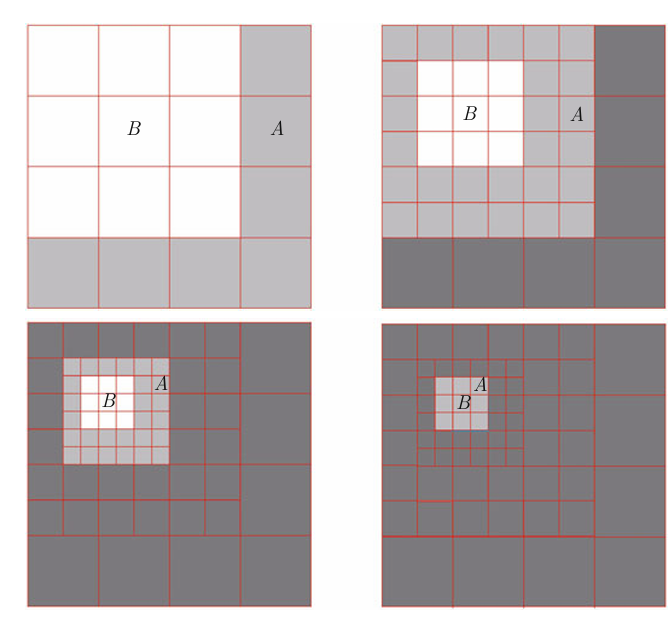
\includegraphics[width=0.65\textwidth]{img/marcoTeorico/fmm_esquema.png}
    %\fbox{\parbox{0.8\textwidth}{\centering Placeholder: Figura Esquema de la Jerarquía de Celdas y Listas de Interacción}}
    \caption{Esquema de la estructura jerárquica de celdas (e.g., quadtree) y la distinción entre interacciones de campo cercano (directas) y campo lejano (aproximadas mediante expansiones), incluyendo la lista de interacción. Adaptado de~\cite{GreengardRokhlin1987, Ying2012}.}%
    \label{fig:fmm_hierarchy}
\end{figure}

% --- Placeholder para Figura 2 (Operadores) ---
\begin{figure}[H]
    \centering
    \resizebox{0.85\textwidth}{!}{ % Cambia el factor de escala aquí
    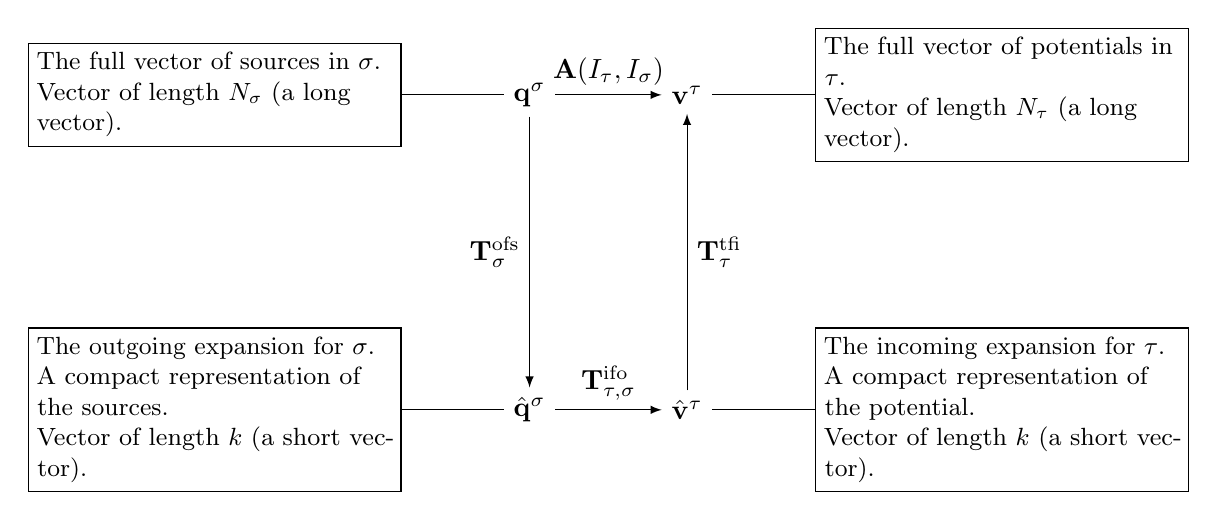
\begin{tikzpicture}[node distance=3cm and 4cm]
        % Define nodes for the vectors
        \node[draw, text width=4.5cm, align=left, font=\small] (q) at (-4, 2) {The full vector of sources in $\sigma$.\\ Vector of length $N_\sigma$ (a long vector).};
        \node[draw, text width=4.5cm, align=left, font=\small] (v) at (6, 2) {The full vector of potentials in $\tau$.\\ Vector of length $N_\tau$ (a long vector).};
        \node[draw, text width=4.5cm, align=left, font=\small] (qhat) at (-4, -2) {The outgoing expansion for $\sigma$.\\ A compact representation of the sources.\\ Vector of length $k$ (a short vector).};
        \node[draw, text width=4.5cm, align=left, font=\small] (vhat) at (6, -2) {The incoming expansion for $\tau$.\\ A compact representation of the potential.\\ Vector of length $k$ (a short vector).};

        % Define intermediate nodes
        \node (qmid) at (0, 2) {$\mathbf{q}^\sigma$};
        \node (vmid) at (2, 2) {$\mathbf{v}^\tau$};
        \node (qhatmid) at (0, -2) {$\hat{\mathbf{q}}^\sigma$};
        \node (vhatmid) at (2, -2) {$\hat{\mathbf{v}}^\tau$};

        % Draw arrows
        \draw[-latex] (qmid) -- (vmid) node[midway, above] {$\mathbf{A}(I_\tau, I_\sigma)$};
        \draw[-latex] (qmid) -- (qhatmid) node[midway, left] {$\mathbf{T}_\sigma^{\text{ofs}}$};
        \draw[-latex] (qhatmid) -- (vhatmid) node[midway, above] {$\mathbf{T}_{\tau,\sigma}^{\text{ifo}}$};
        \draw[-latex] (vhatmid) -- (vmid) node[midway, right] {$\mathbf{T}_\tau^{\text{tfi}}$};

        % Draw lines from boxes to intermediate nodes
        \draw (q) -- (qmid);
        \draw (v) -- (vmid);
        \draw (qhat) -- (qhatmid);
        \draw (vhat) -- (vhatmid);
    \end{tikzpicture}
    }
    \caption{Ilustración del flujo de información en el FMM:\ fuentes originales ($\mathbf{q}^\sigma$) $\rightarrow$ expansión saliente ($\hat{\mathbf{q}}^\sigma$) $\rightarrow$ expansión entrante ($\hat{\mathbf{v}}^\tau$) $\rightarrow$ potenciales ($\mathbf{v}^\tau$), mostrando los operadores T\textsuperscript{ofs}, T\textsuperscript{ifo}, y T\textsuperscript{tfi}. Adaptado de~\cite{Martinsson2012}.}%
    \label{fig:fmm_translations}
\end{figure}


\subsection{Contexto Histórico/Origen}

El FMM fue introducido formalmente por Leslie Greengard y Vladimir Rokhlin en su seminal artículo de 1987~\cite{GreengardRokhlin1987}, aunque ideas relacionadas con expansiones multipolares y métodos jerárquicos existían previamente (e.g.,~\cite{Appel1985, BarnesHut1986}). El trabajo de Greengard y Rokhlin proporcionó un marco riguroso y un algoritmo con complejidad demostrada de $O(N)$ para el problema de Laplace, revolucionando la simulación de $N$-cuerpos y la solución de ecuaciones integrales~\cite{GreengardRokhlin1987}. Su impacto fue tal que fue incluido en la lista de los 10 algoritmos más importantes del siglo XX~\cite{Cipra2000}.

\subsection{Variantes o Enfoques Principales}

El FMM ha evolucionado considerablemente desde su concepción original:
\begin{itemize}
    \item \textbf{Extensiones a otros Kernels:} Aunque inicialmente formulado para el kernel de Laplace ($1/r$), se ha extendido a otros kernels importantes como el de Helmholtz (ondas), Stokes (fluidos), Yukawa (física de partículas) y elasticidad~\cite{ChengEtAl1999, Martinsson2012, Rokhlin1990}. Para kernels oscilatorios como el de Helmholtz, se requieren enfoques más sofisticados (e.g., \textit{FMM direccional}) para mantener la eficiencia, especialmente a altas frecuencias~\cite{EngquistYing2009, Rokhlin1990}.
    \item \textbf{Métodos Adaptativos:} Para manejar distribuciones de partículas altamente no uniformes, se desarrollaron versiones adaptativas del FMM que refinan el árbol jerárquico solo donde es necesario, manteniendo la eficiencia~\cite{CarrierEtAl1988, ChengEtAl1999}.
    \item \textbf{FMM Independiente del Kernel (KIFMM):} Estos métodos buscan separar la maquinaria del FMM (árbol, traslaciones) de las expansiones específicas del kernel, utilizando representaciones intermedias como cargas equivalentes/ficticias y potenciales de chequeo, lo que facilita su aplicación a nuevos kernels~\cite{YingEtAl2004, Martinsson2012}.
    \item \textbf{Optimizaciones para Baja Precisión:} En campos como la astrofísica, donde no siempre se requiere alta precisión, se han desarrollado métodos FMM-like o variantes de códigos de árbol optimizados, que pueden lograr complejidades $O(N)$ o incluso sublineales empíricamente~\cite{Dehnen2002}. El método de Dehnen~\cite{Dehnen2002}, por ejemplo, utiliza interacciones celda-celda y expansiones de Taylor, conservando el momento lineal.
    \item \textbf{Versiones Paralelas y para GPU:} Se han desarrollado implementaciones altamente optimizadas para arquitecturas paralelas modernas, incluyendo CPUs multi-núcleo y GPUs, lo que permite abordar problemas de escala masiva~\cite{YokotaBarba2012, Martinsson2012}.
\end{itemize}

\subsection{Aplicaciones Típicas}

El FMM es una herramienta esencial en:
\begin{itemize}
    \item \textbf{Astrofísica:} Simulación de la evolución dinámica de galaxias y cúmulos estelares (interacciones gravitacionales)~\cite{Dehnen2002, Cipra2000}.
    \item \textbf{Dinámica Molecular:} Cálculo de fuerzas electrostáticas y de van der Waals en simulaciones de proteínas y otras biomoléculas~\cite{BeatsonGreengard1997}.
    \item \textbf{Electromagnetismo:} Solución de ecuaciones integrales para el cálculo de capacitancia, dispersión de ondas electromagnéticas y diseño de antenas~\cite{ChengEtAl1999, Martinsson2012}.
    \item \textbf{Mecánica de Fluidos:} Simulación de flujos utilizando métodos de vórtices o resolviendo ecuaciones integrales para flujos de Stokes~\cite{BeatsonGreengard1997}.
    \item \textbf{Método de Elementos de Contorno (BEM):} Aceleración de la solución de sistemas lineales densos que surgen de la discretización de ecuaciones integrales de contorno~\cite{ChenSF, Martinsson2012}.
\end{itemize}

\subsection{Ventajas y Desventajas/Limitaciones}

\textbf{Ventajas:}
\begin{itemize}
    \item \textbf{Eficiencia Asintótica:} Su complejidad $O(N)$ o $O(N \log N)$ lo hace significativamente más rápido que los métodos directos $O(N^2)$ para $N$ grande~\cite{GreengardRokhlin1987}.
    \item \textbf{Precisión Controlable:} La exactitud de la aproximación se puede ajustar sistemáticamente aumentando el orden $p$ de las expansiones~\cite{BeatsonGreengard1997}.
    \item \textbf{Escalabilidad:} Las versiones modernas han demostrado una excelente escalabilidad en arquitecturas paralelas de alto rendimiento~\cite{YokotaBarba2012}.
    \item \textbf{Amplia Aplicabilidad:} Existen variantes para una gran diversidad de kernels de interacción física~\cite{Martinsson2012}.
\end{itemize}

\textbf{Desventajas/Limitaciones:}
\begin{itemize}
    \item \textbf{Complejidad de Implementación:} El algoritmo es considerablemente más complejo de implementar y depurar que los métodos directos o códigos de árbol más simples~\cite{BeatsonGreengard1997, Martinsson2012}.
    \item \textbf{Constante Oculta:} Aunque asintóticamente eficiente, la constante multiplicativa en la complejidad $O(N)$ puede ser grande, haciendo que para valores pequeños o intermedios de $N$, métodos más simples (como Barnes-Hut o incluso directos) puedan ser competitivos~\cite{Dehnen2002}.
    \item \textbf{Consumo de Memoria:} Requiere almacenar las expansiones multipolares y locales en cada celda del árbol, lo que puede incrementar el uso de memoria en comparación con métodos directos~\cite{YingEtAl2004}.
    \item \textbf{Rendimiento en Distribuciones No Uniformes:} Las versiones no adaptativas pueden perder eficiencia si la distribución de partículas es muy irregular, aunque las variantes adaptativas mitigan este problema~\cite{CarrierEtAl1988, ChengEtAl1999}.
\end{itemize}

% --- Placeholder para Tabla (Comparación Complejidad) ---
\begin{table}[H]
    \centering
    \caption{Comparación de complejidad computacional para problemas de N-cuerpos.}%
    \label{tab:fmm_complexity}
    \begin{tabular}{lc}
        \hline
        \textbf{Método} & \textbf{Complejidad Computacional} \\
        \hline
        Cálculo Directo & $O(N^2)$ \\
        Algoritmo Barnes-Hut & $O(N \log N)$ \\
        Método Multipolar Rápido (FMM) & $O(N)$ o $O(N \log N)$ \\
        % FMM (Estimación precisa, d dims) & $O(N \log^{(d-1)}(1/\epsilon))$ \\ % Opcional
        \hline
    \end{tabular}\\
    \medskip \small Fuente: Basado en~\cite{GreengardRokhlin1987, BeatsonGreengard1997, Martinsson2012}.
\end{table}

    \subsection{Simulación Barnes-Hut}%
\label{sec:barnes_hut}

La simulación Barnes-Hut es un algoritmo de aproximación ampliamente utilizado en el campo de la física computacional, especialmente en astrofísica, para simular la evolución dinámica de sistemas de N-cuerpos (\textit{N-body systems}) bajo la influencia de fuerzas de largo alcance, como la gravedad o las interacciones electrostáticas~\cite{Barnes1986, dubinski1996}. Fue propuesto originalmente por Josh Barnes y Piet Hut en 1986~\cite{Barnes1986} como una solución eficiente al problema computacionalmente intensivo del cálculo directo de todas las interacciones por pares en un sistema grande, cuya complejidad escala como $O(N^2)$. El algoritmo Barnes-Hut reduce esta complejidad a $O(N \log N)$, permitiendo la simulación de sistemas con un número significativamente mayor de partículas~\cite{Barnes1986, salmon1991}.

\subsubsection{Principios y Funcionamiento}

El principio fundamental del algoritmo Barnes-Hut radica en la aproximación de la fuerza ejercida por un grupo distante de partículas tratándolo como una única pseudo-partícula (o un conjunto de momentos multipolares de bajo orden) ubicada en el centro de masa (CoM) del grupo~\cite{Barnes1986, barnes1990}. Esta aproximación es válida porque el campo gravitatorio (o electrostático) de un grupo de partículas a gran distancia se asemeja al de una sola partícula puntual con la masa total del grupo ubicada en su centro de masa~\cite{pfalzner1996}.

Para implementar esta idea, el algoritmo emplea una estructura de datos jerárquica basada en la subdivisión recursiva del espacio:

\begin{enumerate}
    \item \textbf{Construcción del Árbol (\textit{Tree Construction}):} El espacio que contiene las N partículas se subdivide recursivamente en celdas. En 3D, se utiliza un \textit{octree} (árbol óctuple), donde el cubo que engloba todo el sistema se divide en ocho subcubos (octantes) iguales. Este proceso se repite para cada subcubo que contenga más de una partícula, hasta que cada celda hoja (nodo terminal del árbol) contenga como máximo una partícula~\cite{Barnes1986, dubinski1996}. En 2D, se utiliza una estructura análoga llamada \textit{quadtree} (árbol cuádruple)~\cite{aguirre2020, munier2020}. Cada nodo interno del árbol almacena información agregada sobre las partículas contenidas en su celda correspondiente, como la masa total y la posición del centro de masa~\cite{Barnes1986, salmon1991}.

    \item \textbf{Cálculo de Fuerzas (\textit{Force Calculation}):} Para calcular la fuerza neta sobre una partícula específica $i$, se recorre el árbol desde la raíz. Para cada nodo (celda) $c$ encontrado durante el recorrido, se aplica el \textit{criterio de apertura de Barnes-Hut} (\textit{Barnes-Hut opening criterion}). Este criterio compara el tamaño de la celda $s$ (usualmente su anchura o diagonal) con la distancia $d$ entre la partícula $i$ y el centro de masa de la celda $c$. Si la relación $s/d$ es menor que un parámetro de precisión umbral $\theta$ (theta), es decir:
    \[ s / d < \theta \]
    la celda $c$ se considera ``suficientemente lejana''. En este caso, la contribución a la fuerza sobre la partícula $i$ debida a todas las partículas dentro de la celda $c$ se aproxima utilizando la masa total y el centro de masa (o una expansión multipolar de bajo orden) almacenados en el nodo $c$~\cite{Barnes1986, salmon1991, barnes1990}. Si la condición no se cumple ($s/d \ge \theta$), la celda está demasiado cerca o es demasiado grande para ser aproximada con precisión, por lo que el algoritmo desciende recursivamente a los hijos de ese nodo (si es un nodo interno) y repite el proceso~\cite{Barnes1986, barnes1990}. Si el nodo es una hoja que contiene una partícula $j$ (distinta de $i$), la fuerza entre $i$ y $j$ se calcula directamente~\cite{pfalzner1996}. El valor de $\theta$ (típicamente entre 0.5 y 1.2) controla el equilibrio entre precisión y velocidad: valores más pequeños de $\theta$ resultan en cálculos más precisos pero más lentos (más interacciones directas y nodos visitados), mientras que valores más grandes aceleran el cálculo a costa de una menor precisión~\cite{barnes1990, aguirre2020}.
\end{enumerate}

\subsubsection{Contexto Histórico y Origen}

El algoritmo fue presentado por Josh Barnes y Piet Hut en su artículo de 1986 en la revista \textit{Nature}, titulado ``A hierarchical $O(N \log N)$ force-calculation algorithm''~\cite{Barnes1986}. Su desarrollo fue motivado por la necesidad de superar las limitaciones computacionales de las simulaciones N-cuerpos directas en astrofísica, que impedían estudiar sistemas a gran escala como la formación y dinámica de galaxias o cúmulos estelares~\cite{Barnes1986, dubinski1996}. El algoritmo Barnes-Hut representó un avance significativo al hacer factibles simulaciones con cientos de miles o millones de partículas en la época.

\subsubsection{Variantes y Enfoques Principales}

Desde su concepción, el algoritmo Barnes-Hut ha sido objeto de diversas optimizaciones y variantes:

\begin{itemize}
    \item \textbf{Implementaciones Paralelas:} Dada la naturaleza jerárquica y divisible del problema, el algoritmo se adapta bien a la paralelización. Se han desarrollado diversas estrategias para distribuir la construcción del árbol y el cálculo de fuerzas entre múltiples procesadores o nodos de cómputo, utilizando técnicas como la descomposición de dominio (ej.\ \textit{Bisección Recursiva Ortogonal \- ORB}~\cite{salmon1991}) o la distribución de partículas basada en carga computacional~\cite{dubinski1996, becciani1997, becciani2000}.
    \item \textbf{Aceleración por GPU:} Las unidades de procesamiento gráfico (GPUs), con su arquitectura masivamente paralela, han demostrado ser muy eficaces para acelerar las simulaciones Barnes-Hut~\cite{burtscher2011, hamada2009}. Existen implementaciones donde partes significativas o la totalidad del algoritmo se ejecutan en la GPU~\cite{burtscher2011}.
    \item \textbf{Expansiones Multipolares:} Para mejorar la precisión de la aproximación de fuerzas de grupos distantes, en lugar de usar solo el monopolo (masa total y CoM), se pueden incluir términos de orden superior como el cuadrupolo~\cite{barnes1990, salmon1994}. Esto es especialmente relevante cuando se requiere una alta fidelidad en la simulación.
    \item \textbf{Combinación con otros Métodos:} En algunas simulaciones cosmológicas a gran escala, el algoritmo Barnes-Hut puede combinarse con métodos de malla de partículas (\textit{Particle-Mesh}, PM) para manejar las fuerzas de largo alcance de manera eficiente, mientras que Barnes-Hut se encarga de las interacciones a corta y mediana escala~\cite{bagla2004}.
    \item \textbf{Optimización de Árboles:} Se han explorado variantes en la construcción y recorrido del árbol, como los árboles \textit{k-d} o el uso de árboles duales (\textit{dual-tree}) que recorren simultáneamente dos árboles para optimizar el cálculo de interacciones celda-celda en lugar de partícula-celda~\cite{vandemaaten2008, vandermaaten2013}.
\end{itemize}

\subsubsection{Aplicaciones Típicas}

El algoritmo Barnes-Hut y sus variantes se aplican en diversos campos científicos y técnicos:

\begin{itemize}
    \item \textbf{Astrofísica:} Es una herramienta estándar para simulaciones de formación y evolución de galaxias, interacciones galácticas, dinámica de cúmulos estelares y globulares, y formación de estructuras a gran escala en cosmología~\cite{dubinski1996, salmon1991, bagla2004}.
    \item \textbf{Dinámica Molecular:} Se utiliza para calcular eficientemente las interacciones electrostáticas y de Van der Waals (que también son de largo alcance) en simulaciones de sistemas moleculares grandes como proteínas, ADN o fluidos iónicos~\cite{pfalzner1996, Gan2014}.
    \item \textbf{Física de Plasmas:} Para simular la interacción entre partículas cargadas en plasmas~\cite{winkel2012}.
    \item \textbf{Visualización de Datos y Aprendizaje Automático:} Se ha adaptado para acelerar algoritmos de reducción de dimensionalidad y visualización, como t-SNE (\textit{t-distributed Stochastic Neighbor Embedding}), donde se modelan ``fuerzas'' atractivas y repulsivas entre puntos de datos en un espacio de baja dimensión~\cite{vandemaaten2008, vandermaaten2013}.
    \item \textbf{Graficación por Computadora y Diseño de Grafos:} Para algoritmos de diseño dirigido por fuerzas (\textit{force-directed layout}), donde los nodos de un grafo se repelen y las aristas actúan como resortes, buscando una disposición espacial estéticamente agradable o funcional~\cite{Nguyen2007}.
\end{itemize}

\subsubsection{Ventajas y Limitaciones}

\paragraph{Ventajas}
\begin{itemize}
    \item \textbf{Eficiencia Computacional:} Su complejidad $O(N \log N)$ permite simular sistemas mucho más grandes que los métodos directos $O(N^2)$~\cite{Barnes1986}.
    \item \textbf{Versatilidad:} Aplicable a diferentes tipos de fuerzas de largo alcance (gravitatoria, electrostática)~\cite{pfalzner1996, Gan2014}.
    \item \textbf{Adaptabilidad:} La estructura de árbol se adapta naturalmente a distribuciones de partículas no uniformes (clusterizadas)~\cite{becciani1997, dubinski1996}.
    \item \textbf{Paralelizable:} Se presta bien a la implementación en arquitecturas de cómputo paralelo (multi-núcleo, GPU, clusters)~\cite{dubinski1996, burtscher2011}.
\end{itemize}

\paragraph{Limitaciones}
\begin{itemize}
    \item \textbf{Aproximación:} Introduce errores en el cálculo de fuerzas, cuya magnitud depende del parámetro $\theta$ y de la distribución de partículas~\cite{barnes1990, aguirre2020}. No es adecuado para simulaciones que requieran una precisión extremadamente alta en las interacciones individuales (ej.\ dinámica de sistemas planetarios precisos a largo plazo).
    \item \textbf{Complejidad de Implementación:} Aunque conceptualmente más simple que otros métodos rápidos como el Método Multipolo Rápido (FMM), su implementación correcta, especialmente las versiones paralelas u optimizadas, requiere un esfuerzo considerable~\cite{dubinski1996, salmon1991}.
    \item \textbf{Coste de Construcción del Árbol:} La construcción (o reconstrucción) del árbol en cada paso de tiempo representa una sobrecarga computacional que no existe en los métodos directos~\cite{salmon1991}.
    \item \textbf{Condiciones de Contorno:} La implementación de condiciones de contorno periódicas, comunes en cosmología o dinámica molecular, es más compleja que en métodos basados en mallas~\cite{bagla2004}.
\end{itemize}

    \section[REBOUND]{REBOUND:\ Código N-cuerpos multipropósito de código abierto para dinámica colisional}

REBOUND (Rein \& Liu, 2012)~\cite{Rein2012} se define como un código numérico de N-cuerpos, multipropósito y de código abierto, distribuido bajo la licencia GPLv3~\cite{Rein2012}. Fue diseñado primordialmente para abordar problemas de dinámica colisional, como los encontrados en anillos planetarios, pero es igualmente capaz de resolver el problema clásico de N-cuerpos en sistemas puramente gravitacionales~\cite{Rein2012} [Abstract, Sec. 1]. Su desarrollo buscó llenar un vacío existente en cuanto a códigos públicos disponibles para la simulación de dinámica colisional compleja~\cite{Rein2012} [Sec. 1].

\subsection{Principios Fundamentales y Funcionamiento}

La filosofía central de REBOUND es su alta modularidad~\cite{Rein2012} [Abstract, Sec. 2.2]. Está escrito enteramente en C (conforme al estándar ISO C99) y diseñado para compilar y ejecutarse en plataformas modernas compatibles con POSIX (como Linux, Unix y Mac OSX)~\cite{Rein2012} [Sec. 2, Sec. 2.1]. La estructura modular permite al usuario seleccionar y combinar diferentes componentes mediante el uso de enlaces simbólicos, sin necesidad de modificar el código fuente principal. Esto facilita la adaptación del código a una amplia variedad de problemas astrofísicos y de otras disciplinas~\cite{Rein2012} [Sec. 2.2]. Los módulos intercambiables incluyen:

\begin{enumerate}
    \item \textbf{Integradores Numéricos:} REBOUND implementa varios integradores, mayormente basados en el esquema simpléctico de segundo orden Drift-Kick-Drift (DKD). Es importante notar que la naturaleza simpléctica se pierde formalmente si se introducen aproximaciones en el cálculo de la gravedad, colisiones o fuerzas dependientes de la velocidad~\cite{Rein2012} [Sec. 3]. Los integradores principales son:
    \begin{itemize}
        \item \textbf{Leap-frog:} Un integrador simpléctico estándar de segundo orden para marcos no rotacionales~\cite{Rein2012} [Sec. 3.1].
        \item \textbf{Wisdom-Holman (WH):} Un mapeo simpléctico de variables mixtas que integra el movimiento kepleriano de forma exacta durante el paso de deriva (\textit{drift}). Es muy preciso para problemas dominados por un potencial central $1/r$, pero computacionalmente más costoso que Leap-frog debido a la resolución iterativa de la ecuación de Kepler~\cite{Rein2012} [Sec. 3.2].
        \item \textbf{Symplectic Epicycle Integrator (SEI):} Diseñado para la aproximación de Hill (utilizada en láminas de cizallamiento o \textit{shearing sheets}), opera en un marco rotacional y es computacionalmente rápido~\cite{Rein2012} [Sec. 3.3].
    \end{itemize}
    REBOUND utiliza un paso de tiempo (\textit{timestep}) fijo para todas las partículas por defecto, lo cual es crucial para mantener las propiedades simplécticas de los integradores correspondientes. Es responsabilidad del usuario asegurar que el paso de tiempo sea suficientemente pequeño para la convergencia numérica~\cite{Rein2012} [Sec. 3].

    \item \textbf{Cálculo de Gravedad:} Se proporcionan dos módulos principales para calcular las fuerzas gravitacionales~\cite{Rein2012} [Sec. 4]:
    \begin{itemize}
        \item \textbf{Suma Directa:} Calcula la interacción entre todos los pares de partículas activas ($N_{\text{active}}$) de forma exacta (ecuación 1 en~\cite{Rein2012}). Su costo computacional escala como $O(N \cdot N_{\text{active}})$, siendo eficiente solo para un número bajo de partículas masivas ($N_{\text{active}} \le 10^2$)~\cite{Rein2012} [Sec. 4.1]. Permite incluir un parámetro de suavizado gravitacional ($b$) para evitar aceleraciones extremas en encuentros cercanos~\cite{Rein2012} [Eq. 1].
        \item \textbf{Octree (Árbol Octal):} Implementa el algoritmo de Barnes \& Hut (1986) para aproximar las fuerzas de largo alcance, reduciendo la complejidad computacional a $O(N \log N)$~\cite{Rein2012} [Sec. 4.2]. Agrupa jerárquicamente las partículas distantes y utiliza su centro de masa (y opcionalmente su tensor cuadrupolar, siguiendo a Hernquist, 1987) para calcular la fuerza, basándose en un criterio de ángulo de apertura ($\theta_{\text{crit}}$). Este módulo está completamente paralelizado usando MPI (con descomposición estática de dominio y árboles esenciales distribuidos) y OpenMP~\cite{Rein2012} [Sec. 4.2, Sec. 7].
        % Sugerencia Visual:
        % [Aquí podría insertarse una figura adaptada de la Fig. 4 de~\cite{Rein2012} para ilustrar la convergencia
        % de la precisión de la fuerza en función de theta_crit y la mejora al incluir el término cuadrupolar].
    \end{itemize}

    \item \textbf{Detección de Colisiones:} REBOUND incluye varios módulos para detectar colisiones, modeladas como interacciones entre esferas duras con un coeficiente de restitución $\epsilon$ especificado por el usuario~\cite{Rein2012} [Sec. 5]. Las colisiones detectadas en un paso de tiempo se resuelven en orden aleatorio para evitar sesgos~\cite{Rein2012} [Sec. 5]. Los métodos son:
    \begin{itemize}
        \item \textbf{Búsqueda Directa del Vecino Más Cercano:} Comprueba el solapamiento de todas las parejas de partículas al final del paso de tiempo. Escala como $O(N^2)$~\cite{Rein2012} [Sec. 5.1].
        \item \textbf{Octree:} Utiliza la estructura del árbol octal para buscar vecinos cercanos y detectar solapamientos, con una complejidad promedio de $O(N \log N)$. Puede usar la misma estructura del árbol de gravedad y está paralelizado (MPI/OpenMP)~\cite{Rein2012} [Sec. 5.2].
        \item \textbf{Algoritmo de Barrido Plano (Plane-Sweep):} Dos variantes (cartesiana en $x$ y angular en $\phi$) basadas en el algoritmo de Bentley \& Ottmann (1979), pero simplificadas. Aproxima las trayectorias de las partículas como líneas rectas durante un paso de tiempo. Mueve un plano conceptual a través del dominio, manteniendo una lista de partículas activas intersectadas por el plano y comprobando colisiones solo dentro de esa lista. Su complejidad es $O(N \cdot N_{\text{SWEEPL}})$, donde $N_{\text{SWEEPL}}$ es el número promedio de partículas en la lista activa. Es significativamente más eficiente que los métodos basados en árboles para simulaciones cuasi-bidimensionales o muy elongadas (donde $N_{\text{SWEEPL}}$ es pequeño), como anillos planetarios densos o simulaciones en láminas de cizallamiento~\cite{Rein2012} [Sec. 5.3].
        \begin{figure}[H]
            \centering
            % Descomenta la siguiente línea e inserta la ruta a tu imagen
            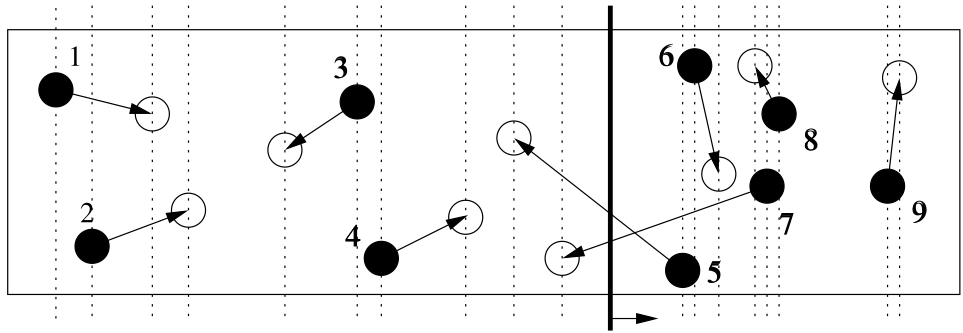
\includegraphics[width=\textwidth]{img/marcoTeorico/Algoritmo_de_barrido_plano.png}
            %\fbox{\parbox{0.8\textwidth}{\centering Placeholder: Figura Esquema de la Jerarquía de Celdas y Listas de Interacción}}
            \caption{Ilustración del algoritmo de barrido plano. El plano interseca las trayectorias de las partículas 5 y 7. Véanse los detalles en el texto adaptado de~\cite{Rein2012}.}%
            \label{fig:plane_sweep_algorithm}
        \end{figure}
    \end{itemize}

    \item \textbf{Condiciones de Contorno:} Soporta condiciones de contorno abiertas (las partículas que salen son eliminadas), periódicas (implementadas con cajas fantasma) y de lámina de cizallamiento (\textit{shear-periodic})~\cite{Rein2012} [Sec. 2.3].
\end{enumerate}

\subsection{Contexto Histórico y Origen}

El código fue presentado por H. Rein y S.-F. Liu en 2012~\cite{Rein2012}, aunque versiones precursoras ya se habían utilizado en publicaciones anteriores (e.g., Rein \& Papaloizou, 2010; Crida et al., 2010; Rein et al., 2010)~\cite{Rein2012} [Sec. 1]. Nació de la necesidad de contar con una herramienta pública, flexible y eficiente para estudiar la dinámica de sistemas astrofísicos donde las colisiones juegan un papel crucial, como los anillos de Saturno o los discos protoplanetarios~\cite{Rein2012} [Sec. 1].

\subsection{Variantes y Enfoques Principales}

Más que variantes distintas del código, REBOUND ofrece diferentes enfoques de simulación a través de la combinación de sus módulos. El usuario puede configurar la simulación eligiendo el integrador más adecuado (e.g., WH para alta precisión a largo plazo en sistemas planetarios, SEI para láminas de cizallamiento, Leap-frog como opción general), el método de cálculo de gravedad (directo para pocos cuerpos, árbol para muchos) y el algoritmo de detección de colisiones (directo, árbol, o barrido plano según la geometría y densidad del problema)~\cite{Rein2012} [Sec. 2.2, Sec. 3, Sec. 4, Sec. 5].

\subsection{Aplicaciones Típicas}

La literatura documenta el uso de REBOUND en una variedad de problemas astrofísicos:
\begin{itemize}
    \item Simulación de anillos planetarios, incluyendo el estudio de su viscosidad y estructuras inducidas por satélites~\cite{Rein2012} [Sec. 1, Sec. 6.4].
    \item Formación de planetesimales a partir de enjambres de partículas en discos protoplanetarios~\cite{Rein2012} [Sec. 1].
    \item Estudio de discos de transición y de escombros (utilizando superpartículas)~\cite{Rein2012} [Sec. 1].
    \item Problemas clásicos de N-cuerpos, como la integración a largo plazo de la dinámica del Sistema Solar~\cite{Rein2012} [Sec. 1, Sec. 6.3].
\end{itemize}
Aunque diseñado para astrofísica, su estructura modular lo hace potencialmente aplicable a otros campos que involucren dinámica de partículas, como la dinámica molecular o flujos granulares~\cite{Rein2012} [Abstract].

\subsection{Ventajas y Limitaciones}

Las principales \textbf{ventajas} de REBOUND, según se desprenden de~\cite{Rein2012}, son:
\begin{itemize}
    \item \textbf{Código Abierto y Gratuito:} Accesible para la comunidad científica bajo licencia GPLv3~\cite{Rein2012} [Sec. 1].
    \item \textbf{Modularidad y Flexibilidad:} Altamente personalizable para diferentes problemas~\cite{Rein2012} [Abstract, Sec. 2.2].
    \item \textbf{Eficiencia y Escalabilidad:} Demuestra buen escalado en paralelo (tanto fuerte como débil) usando MPI y OpenMP, permitiendo simulaciones con un gran número de partículas en clústeres de cómputo~\cite{Rein2012} [Abstract, Sec. 7].
    \item \textbf{Variedad de Métodos:} Ofrece múltiples opciones de integradores, cálculo de gravedad y detección de colisiones~\cite{Rein2012} [Sec. 3, Sec. 4, Sec. 5].
    \item \textbf{Precisión:} Los integradores simplécticos son adecuados para integraciones a largo plazo, y se conserva la energía y el momento hasta la precisión de la máquina en colisiones elásticas~\cite{Rein2012} [Sec. 3, Sec. 6.2].
\end{itemize}

Las \textbf{limitaciones} inherentes o aspectos a considerar son:
\begin{itemize}
    \item \textbf{Paso de Tiempo Fijo:} Generalmente requerido por los integradores simplécticos, lo que puede ser ineficiente si ocurren escalas de tiempo muy diferentes en el sistema~\cite{Rein2012} [Sec. 3]. El usuario debe elegirlo cuidadosamente.
    \item \textbf{Pérdida de Simplecticidad:} Las propiedades simplécticas se pierden si se usan aproximaciones (árbol de gravedad), colisiones o fuerzas no conservativas~\cite{Rein2012} [Sec. 3].
    \item \textbf{Aproximaciones:} Los métodos de árbol para gravedad y colisiones son aproximados, con una precisión que depende de parámetros como $\theta_{\text{crit}}$~\cite{Rein2012} [Sec. 4.2, Sec. 6.1]. El método de barrido plano aproxima las trayectorias como líneas rectas entre pasos~\cite{Rein2012} [Sec. 5.3, Fig. 2].
    \item \textbf{Rendimiento:} El rendimiento del árbol puede degradarse si el número de partículas por nodo MPI es muy bajo debido al costo de comunicación~\cite{Rein2012} [Sec. 7.1]. La eficiencia del barrido plano depende crucialmente de la dimensionalidad efectiva del problema~\cite{Rein2012} [Sec. 5.3, Sec. 9].
\end{itemize}

    %\section{Programación Matemática}

% --- El texto de la sección permanece igual ---
% Se usan los mismos comandos~\cite{key} y~\cite[page]{key}

El concepto de Programación Matemática\footnote{\textbf{Programación Matemática:} Rama de las matemáticas aplicadas que se ocupa de la teoría y los métodos para resolver problemas de optimización, es decir, encontrar el mejor valor (máximo o mínimo) de una función objetivo sujeta a un conjunto de restricciones.} constituye una disciplina fundamental y contemporánea dentro del campo de las Matemáticas Aplicadas. Se define como el área dedicada al estudio y desarrollo de la teoría, los algoritmos y las aplicaciones para la resolución de problemas de optimización, donde se busca seleccionar la mejor alternativa entre un conjunto de opciones disponibles, sujeta a un conjunto de restricciones~\cite[p.~1]{sinha2006},~\cite[p.~1]{luenberger1984}. En esencia, la Programación Matemática se enfoca en la identificación y determinación de la solución más ventajosa o eficiente para un problema específico, considerando un conjunto predefinido de restricciones que delinean el espacio de alternativas factibles~\cite[p.~1]{sinha2006}. La optimización, por lo tanto, se erige como el núcleo central de la Programación Matemática, buscando la asignación más efectiva de recursos escasos para alcanzar objetivos concretos.\ \textit{Management Science}\footnote{\textbf{Management Science (Ciencia de la Gestión):} Disciplina que utiliza un enfoque científico, a menudo cuantitativo, para la toma de decisiones gerenciales y la resolución de problemas en organizaciones.} (Ciencia de la Gestión), una disciplina caracterizada por un enfoque científico para la toma de decisiones gerenciales, utiliza la Programación Matemática como una de sus herramientas más poderosas, aplicando métodos matemáticos y las capacidades de las computadoras modernas a los problemas complejos y no estructurados que enfrentan los gestores~\cite[p.~1]{bradley1977applied}.

Desde una perspectiva formal, la Programación Matemática implica la formulación de una representación abstracta del problema a través de un modelo matemático, seguido por la aplicación de algoritmos de optimización para la determinación de los valores óptimos que deben adoptar las variables de decisión dentro de dicho modelo~\cite[p.~175]{bertsekas1999}. Un problema de optimización general se puede plantear como la selección de variables de decisión $x_1, x_2, \ldots, x_n$ de una región factible dada, de tal manera que se optimice (minimice o maximice) una función objetivo $f(x_1, x_2, \ldots, x_n)$~\cite[p.~410]{nocedal2006}.

Los principios fundamentales de la Programación Matemática se estructuran en torno a los componentes esenciales que definen cualquier problema de optimización. Estos incluyen:
\begin{enumerate}
    \item \textbf{Variables de Decisión:} Cantidades que el tomador de decisiones controla y cuyos valores determinan la solución del modelo~\cite[p.~181]{bradley1977applied}.
    \item \textbf{Función Objetivo:} Una medida de rendimiento o efectividad, expresada como una función matemática de las variables de decisión, que se busca maximizar o minimizar~\cite[p.~181]{bradley1977applied}.
    \item \textbf{Restricciones:} Un conjunto de relaciones (ecuaciones o inecuaciones) que las variables de decisión deben satisfacer, reflejando las limitaciones impuestas por la naturaleza del problema (disponibilidad de recursos, requisitos tecnológicos, etc.)~\cite[p.~181]{bradley1977applied}.
\end{enumerate}

El objetivo primordial es, por lo tanto, determinar los valores óptimos de las variables de decisión que no solo satisfacen todas las restricciones impuestas al sistema, sino que también logran el mejor valor posible para la función objetivo.

El desarrollo formal de la Programación Matemática, especialmente la Programación Lineal, se consolidó a mediados del siglo XX.\ George B. Dantzig es ampliamente reconocido por el desarrollo del \textit{algoritmo simplex} alrededor de 1947, que proporcionó un método sistemático y eficiente para resolver problemas de Programación Lineal~\cite[p.~2]{sinha2006},~\cite[p.~1]{bradley1977applied}. Este avance fue un punto de inflexión, impulsado en gran medida por la necesidad de optimizar la asignación de recursos durante la Segunda Guerra Mundial en el contexto de la \textit{Investigación Operativa}\footnote{\textbf{Investigación Operativa (Operations Research):} Disciplina que aplica métodos analíticos avanzados para ayudar a tomar mejores decisiones. Surgió durante la Segunda Guerra Mundial para resolver problemas militares complejos.} (Operations Research)~\cite[p.~1]{sinha2006}. Sin embargo, los fundamentos de la optimización se pueden rastrear a trabajos mucho anteriores de matemáticos como Lagrange y Fourier~\cite[p.~1]{sinha2006}. En la década de 1950, surgieron avances significativos en Programación No Lineal con las contribuciones de Kuhn y Tucker sobre condiciones de optimalidad, y en Programación Dinámica gracias a Richard Bellman~\cite[p.~9]{sinha2006}. Ralph Gomory realizó trabajos pioneros en Programación Entera durante el mismo período~\cite[p.~9]{sinha2006}.

\subsection{Variantes Principales de la Programación Matemática}

La Programación Matemática abarca diversas variantes, cada una diseñada para tipos específicos de problemas:

\begin{enumerate}[label=\arabic*.]
    \item \textbf{Programación Lineal (PL):}
    Se caracteriza porque tanto la función objetivo como todas las restricciones son funciones lineales de las variables de decisión~\cite[p.~2]{sinha2006},~\cite[p.~9]{bradley1977applied}. Los principios fundamentales de la PL incluyen la proporcionalidad (la contribución de cada variable es proporcional a su valor), la aditividad (la contribución total es la suma de las contribuciones individuales), la divisibilidad (las variables pueden tomar valores fraccionarios) y la certeza (todos los parámetros del modelo son conocidos con exactitud)~\cite[p.~9]{bradley1977applied}. La forma general de un problema de PL es: \\
    Optimizar $z = \sum_{j=1}^{n} c_j x_j$ \\
    Sujeto a:
    \begin{align*}
        \sum_{j=1}^{n} a_{ij} x_j & (\leq, =, \geq) b_i, && \text{para } i = 1, \ldots, m_1+m_2+m_3 \\
        x_j & \geq 0 && \text{(para algunas o todas las } j\text{)} \\ %chktex 9
        x_j & \text{ irrestricta} && \text{(para algunas o todas las } j\text{)} %chktex 9
    \end{align*}
~\cite[p.~117]{sinha2006}. \\
    \begin{figure}
        \centering
        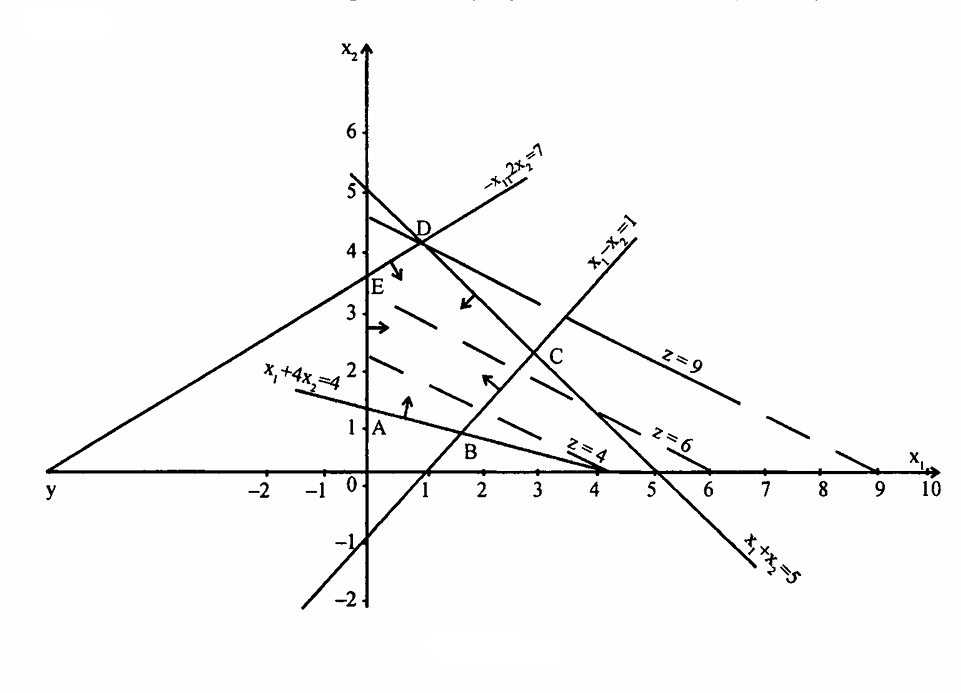
\includegraphics[width=0.75\linewidth]{img/marcoTeorico/mathprogramming_fig1.png}
        \caption{Representación bidimensional de la región factible de un problema de programación lineal, caracterizada por un polígono convexo definido por restricciones lineales. Se incluyen líneas de nivel de la función objetivo y el punto óptimo ubicado en un vértice del conjunto factible, ilustrando la solución típica en problemas lineales. Adaptado de~\cite[p.~6-7]{sinha2006}}%
        \label{fig:mathprogramming01}
    \end{figure}

    \item \textbf{Programación No Lineal (PNL):}
    Se aplica cuando la función objetivo o al menos una de las restricciones (o ambas) es una función no lineal de las variables de decisión~\cite[p.~9]{sinha2006},~\cite[p.~410]{nocedal2006}. A diferencia de la PL, donde el óptimo (si existe) se encuentra en un vértice de la región factible, en PNL el óptimo puede estar en el interior de la región, en su frontera (no necesariamente un vértice), o en un vértice~\cite[p.~413, Figura 13.1]{nocedal2006}. Una distinción crucial en PNL es entre óptimos locales y globales. Un óptimo local es una solución mejor que todas las soluciones ``cercanas'', mientras que un óptimo global es la mejor solución en toda la región factible~\cite[p.~413]{nocedal2006}. \\

    \begin{figure}
        \centering
        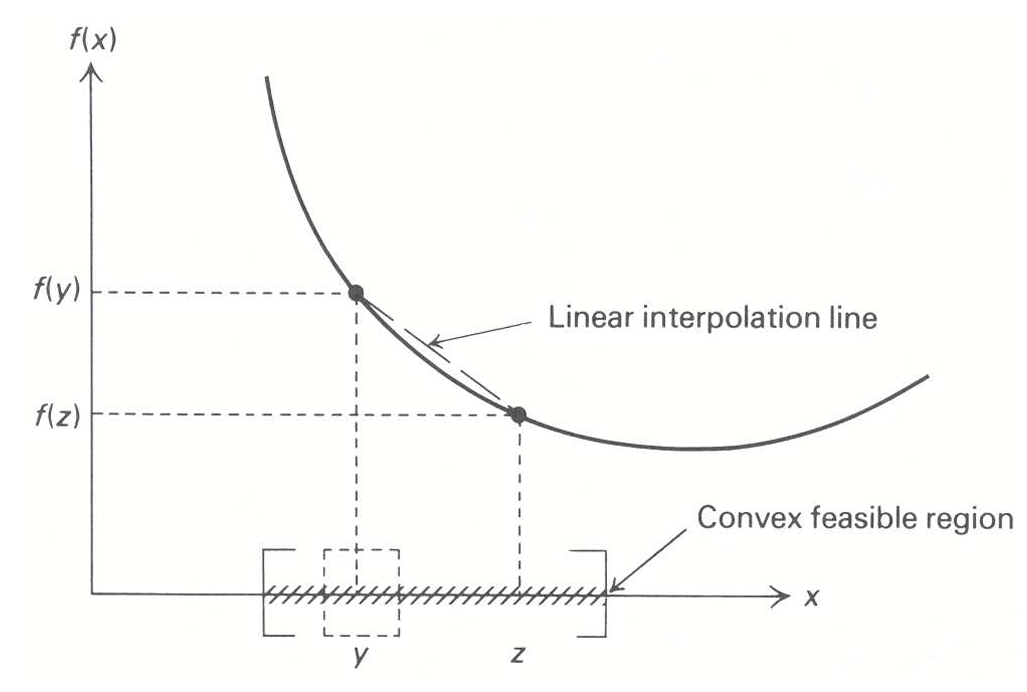
\includegraphics[width=0.75\linewidth]{img/marcoTeorico/mathprogramming_fig2.png}
        \caption{Visualización de una función no lineal con múltiples extremos locales y un único óptimo global, empleada para ilustrar las diferencias conceptuales entre mínimos (o máximos) locales y globales en problemas de programación no lineal. Esta distinción es clave en el análisis de algoritmos de optimización y su convergencia. Adaptado de~\cite[p.~419]{bradley1977applied}}%
        \label{fig:mathprogramming01}
    \end{figure}

    Dentro de la PNL, la \textit{Programación Convexa} es de particular importancia. Si un problema de minimización involucra minimizar una función convexa sobre un conjunto convexo, o un problema de maximización implica maximizar una función cóncava sobre un conjunto convexo, entonces cualquier óptimo local es también un óptimo global~\cite[p.~418]{nocedal2006},~\cite[p.~1]{boyd2004}.
    \begin{itemize}
        \item \textbf{Programación Cuadrática:} Un caso especial de PNL donde la función objetivo es cuadrática y las restricciones son lineales~\cite[p.~419]{nocedal2006}. Su forma general es: \\
        Maximizar $f(x) = \sum_{j=1}^{n} c_j x_j + \frac{1}{2} \sum_{j=1}^{n} \sum_{k=1}^{n} q_{jk} x_j x_k$ \\
        Sujeto a:
        \begin{align*}
            \sum_{j=1}^{n} a_{ij} x_j & \leq b_i, && \text{para } i = 1, \ldots, m \\
            x_j & \geq 0, && \text{para } j = 1, \ldots, n
        \end{align*}~\cite[p.~433]{nocedal2006}.
    \end{itemize}

    \item \textbf{Programación Entera (PE):}
    Se caracteriza porque algunas o todas las variables de decisión están restringidas a tomar valores enteros~\cite[p.~9]{sinha2006},~\cite[p.~272]{bradley1977pe}. Si todas las variables son enteras, se denomina \textit{Programación Entera Pura}; si solo algunas lo son, es \textit{Programación Entera Mixta}. Un caso especial importante es la \textit{Programación Binaria} o \textit{Programación 0\-1}, donde las variables solo pueden tomar los valores 0 o 1, útil para modelar decisiones de tipo sí/no (go/no-go)~\cite[p.~273]{bradley1977pe}. \\

    \item \textbf{Programación Dinámica (PD):}
    Es un enfoque que transforma un problema complejo en una secuencia de subproblemas más simples, interrelacionados. Su característica esencial es la naturaleza multietapa del procedimiento de optimización~\cite[p.~320]{bradley1977pd}. Se basa en el \textit{Principio de Optimalidad de Bellman}: una política óptima tiene la propiedad de que, cualesquiera que sean el estado y la decisión iniciales, las decisiones restantes deben constituir una política óptima con respecto al estado resultante de la primera decisión~\cite[p.~323]{bradley1977pd}. La PD utiliza ecuaciones recursivas para relacionar la solución óptima de un problema de $n$ etapas con la de un problema de $(n-1)$ etapas~\cite[p.~325]{bradley1977pd}.

    \item \textbf{Programación Estocástica:}
    Aborda problemas de optimización donde algunos de los parámetros del modelo (coeficientes de la función objetivo, lado derecho de las restricciones o coeficientes tecnológicos) son inciertos y se representan como variables aleatorias con distribuciones de probabilidad conocidas~\cite[p.~432]{sinha2006}. Los enfoques incluyen la optimización del valor esperado o la incorporación de restricciones probabilísticas (chance constraints).
\end{enumerate}


\subsection{Aplicaciones Típicas}

La Programación Matemática se aplica extensamente en diversos campos:
\begin{itemize}
    \item \textbf{Investigación Operativa:} Planificación de la producción, gestión de inventarios, problemas de transporte y asignación, secuenciación de tareas, optimización de rutas~\cite[p.~3-5]{sinha2006},~\cite[p.~1-2]{bradley1977applied}.
    \item \textbf{Economía y Finanzas:} Optimización de portafolios de inversión, asignación de capital, modelos de equilibrio económico, planificación del desarrollo económico~\cite[p.~100-102]{bradley1977applied},~\cite[p.~411]{nocedal2006}.
    \item \textbf{Ingeniería:} Diseño óptimo de estructuras, planificación de recursos hídricos, optimización de procesos químicos, problemas de carga de redes eléctricas~\cite[p.~412]{nocedal2006}.
    \item \textbf{Logística:} Localización de almacenes, diseño de redes de distribución, gestión de cadenas de suministro~\cite[p.~274]{bradley1977pe}.
\end{itemize}

En el ámbito de la física computacional y la simulación, aunque el término no siempre se use explícitamente, la optimización es fundamental. Por ejemplo, en la minimización de energía en sistemas moleculares, la optimización de parámetros en modelos físicos, o la búsqueda de configuraciones óptimas en simulaciones de N-cuerpos. Los métodos de Programación Matemática, como la Programación Cuadrática, son relevantes para problemas de ajuste de curvas (regresión restringida) en el análisis de datos experimentales~\cite[p.~412]{nocedal2006}.

\subsection{Ventajas y Desventajas}

\begin{itemize}
    \item \textbf{Ventajas:}
    \begin{itemize}
        \item Proporciona un marco estructurado para la toma de decisiones y la optimización de recursos limitados~\cite[p.~182]{bradley1977applied}.
        \item Permite modelar sistemas complejos y encontrar soluciones óptimas o cercanas a la óptima que pueden no ser intuitivas~\cite[p.~183]{bradley1977applied}.
        \item La teoría de la dualidad y el análisis de sensibilidad ofrecen información valiosa sobre el valor de los recursos (precios sombra) y la robustez de la solución ante cambios en los parámetros del modelo~\cite[p.~78-91]{bradley1977applied}.
        \item La disponibilidad de software eficiente permite resolver problemas de gran escala, especialmente en Programación Lineal~\cite[p.~182]{bradley1977applied}.
    \end{itemize}

    \item \textbf{Desventajas/Limitaciones:}
    \begin{itemize}
        \item La formulación de un modelo matemático preciso puede ser compleja y consumir mucho tiempo, requiriendo una comprensión profunda del problema y de las técnicas de modelado~\cite[p.~183]{bradley1977applied}.
        \item Para problemas no lineales no convexos, los algoritmos pueden converger a óptimos locales en lugar de globales~\cite[p.~413]{nocedal2006}.
        \item La Programación Entera, especialmente para problemas grandes, puede ser computacionalmente muy demandante (``NP-hard'')~\cite[p.~287]{bradley1977pe}.
        \item La suposición de certeza en los parámetros (en modelos determinísticos) puede no reflejar la realidad; aunque la Programación Estocástica aborda esto, incrementa la complejidad del modelo~\cite[p.~432]{sinha2006}.
        \item La calidad de la solución depende críticamente de la calidad y disponibilidad de los datos~\cite[p.~183]{bradley1977applied}.
    \end{itemize}
\end{itemize}

    %% Sección principal: Problemas de Factibilidad y Optimización
\section{Problemas de Factibilidad y Optimización}\label{sec:main_fact_opt}

Los problemas de factibilidad y optimización son pilares fundamentales en la modelización y resolución de una
vasta gama de desafíos en la ingeniería, las ciencias computacionales, la economía y la investigación operativa.
Un problema de optimización, en su forma más general, busca seleccionar la ``mejor'' alternativa de un conjunto
de opciones posibles, sujeta a ciertas limitaciones~\cite[p.~1]{BoydVandenberghe2004},~\cite[p.~4]{BoydVandenbergheSlides2023}. Por otro lado, un problema de factibilidad se centra en determinar
si existe al menos una solución que satisfaga un conjunto dado de restricciones, sin considerar necesariamente
un criterio de optimalidad~\cite[p.~130]{BoydVandenberghe2004},~\cite[p.~1]{Sidford2020}. Esta sección definirá
formalmente ambos tipos de problemas, explorará su interrelación y cómo los problemas de factibilidad pueden
ser vistos como un subconjunto de los problemas de optimización.

%% Subsección: Problemas de Optimización
\subsection{Problemas de Optimización}\label{sec:opt_problems}

Un \textbf{problema de optimización matemática}\footnote{\textbf{Problema de optimización matemática:}
También conocido como problema de programación matemática. Consiste en seleccionar la mejor solución
(según algún criterio cuantificado por la función objetivo) de un conjunto de alternativas factibles
(definidas por las restricciones)~\cite[p.~1]{BoydVandenberghe2004}.} se puede expresar en su forma
estándar como~\cite[p.~127]{BoydVandenberghe2004},~\cite[p.~89]{BoydVandenbergheSlides2023}:

\begin{align}
  \text{minimizar} \quad & f_0(x) \\
  \text{sujeto a} \quad & g_i(x) \leq 0, \quad i = 1, \dots, m \\
                      & h_j(x) = 0,    \quad j = 1, \dots, p
\end{align}

donde:
\begin{itemize}
    \item $x \in \mathbb{R}^n$ es el \textbf{vector de variables de optimización}\footnote{\textbf{Vector de
          variables de optimización:} El vector $x = (x_1, \dots, x_n)$ contiene las cantidades que se pueden
          elegir o variar para encontrar la solución óptima. La dimensión $n$ es el número de variables escalares~\cite[p.~1]{BoydVandenberghe2004}.} (o variables de decisión).
    \item $f_0: \mathbb{R}^n \to \mathbb{R}$ es la \textbf{función objetivo}\footnote{\textbf{Función objetivo:}
          La función $f_0: \mathbb{R}^n \to \mathbb{R}$ cuyo valor se busca minimizar (o maximizar). Cuantifica
          el rendimiento, costo, utilidad o mérito asociado a una elección particular de las variables de optimización~\cite[p.~1]{BoydVandenberghe2004}.}, la cual se desea minimizar (o maximizar, lo que es equivalente a
          minimizar $-f_0$).
    \item $g_i: \mathbb{R}^n \to \mathbb{R}$, para $i = 1, \dots, m$, son las \textbf{funciones de restricción
          de desigualdad}.
    \item $h_j: \mathbb{R}^n \to \mathbb{R}$, para $j = 1, \dots, p$, son las \textbf{funciones de restricción
          de igualdad} (usualmente deben ser afines en problemas de optimización convexa).
\end{itemize}

El conjunto $\mathcal{D} = \left(\bigcap_{i=0}^m \text{dom}(f_i)\right) \cap \left(\bigcap_{j=1}^p \text{dom}(h_j)\right)$
es el \textbf{dominio} del problema. Un punto $x \in \mathcal{D}$ es \textbf{factible} si satisface todas las
restricciones. El conjunto de todos los puntos factibles se denomina \textbf{conjunto factible} o \textbf{región factible}~\cite[p.~128]{BoydVandenberghe2004},~\cite[p.~90]{BoydVandenbergheSlides2023}. Si el conjunto factible es vacío,
el problema es \textbf{infactible}. El valor $p^* = \inf\{f_0(x) \mid x \text{ es factible}\}$ es el \textbf{valor óptimo}.
Si existe un $x^*$ tal que $f_0(x^*) = p^*$, entonces $x^*$ es un \textbf{punto óptimo} (global)~\cite[p.~128]{BoydVandenberghe2004},~\cite[p.~90]{BoydVandenbergheSlides2023}.

\begin{figure}
    \centering
    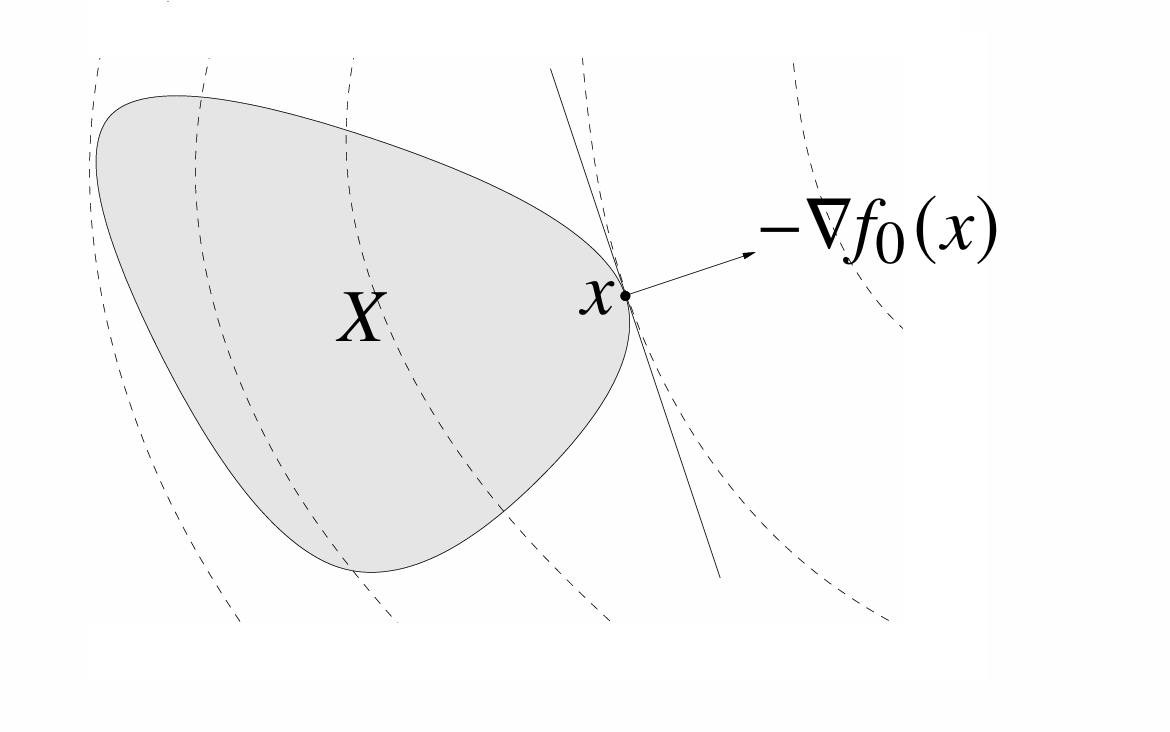
\includegraphics[width=\linewidth]{img//marcoTeorico/optimizacion_fig1.png}
    \caption{Gráfica 2D que muestre contornos de una función objetivo $f_0(x)$,
              una región factible sombreada definida por restricciones, y el punto óptimo $x^*$.}%
    \label{fig:enter-label}
\end{figure}

Los problemas de optimización se clasifican según la naturaleza de sus funciones objetivo y de restricción.
Los \textbf{problemas de programación lineal (LP)}\footnote{\textbf{Programación Lineal (LP):} Un problema de
optimización donde tanto la función objetivo $f_0$ como todas las funciones de restricción $f_i$ y $h_j$ son afines
(lineales más una constante)~\cite[p.~4]{BoydVandenberghe2004},~\cite[p.~101]{BoydVandenbergheSlides2023}.} tienen
funciones objetivo y de restricción afines~\cite[p.~4]{BoydVandenberghe2004},~\cite[p.~101]{BoydVandenbergheSlides2023}.
Los \textbf{problemas de programación cuadrática (QP)}\footnote{\textbf{Programación Cuadrática (QP):} Un problema de
optimización donde la función objetivo $f_0$ es cuadrática (y usualmente convexa para garantizar tratabilidad) y las
funciones de restricción $f_i$ y $h_j$ son afines~\cite[p.~152]{BoydVandenberghe2004},~\cite[p.~105]{BoydVandenbergheSlides2023}.} implican minimizar una función objetivo cuadrática convexa sobre un
poliedro (definido por restricciones afines)~\cite[p.~152]{BoydVandenberghe2004},~\cite[p.~105]{BoydVandenbergheSlides2023}.

Un caso particularmente importante es la \textbf{optimización convexa}, donde la función objetivo $f_0$ y las funciones
de restricción de desigualdad $f_1, \dots, f_m$ son funciones convexas\footnote{\textbf{Función convexa:} Una función
$f: \mathbb{R}^n \to \mathbb{R}$ es convexa si su dominio $\text{dom}(f)$ es un conjunto convexo y para todo $x, y \in \text{dom}(f)$
y todo $\theta$ con $0 \leq \theta \leq 1$, se cumple la desigualdad de Jensen: $f(\theta x + (1 - \theta)y) \leq \theta f(x) + (1 - \theta)f(y)$~\cite[p.~67]{BoydVandenberghe2004},~\cite[p.~46]{BoydVandenbergheSlides2023}. Geométricamente, el segmento de línea que
une dos puntos cualesquiera $(x, f(x))$ e $(y, f(y))$ en la gráfica de la función se encuentra por encima o sobre la gráfica de $f$.},
y las funciones de restricción de igualdad $h_j$ son afines (es decir, de la forma $Ax = b$)~\cite[p.~7]{BoydVandenberghe2004},~\cite[pp.~13, 95]{BoydVandenbergheSlides2023}. La optimización convexa es fundamental
porque, a diferencia de los problemas de optimización no lineal generales, cualquier óptimo local es también un óptimo global,
y existen algoritmos eficientes y confiables para resolverlos~\cite[pp.~8-9]{BoydVandenberghe2004},~\cite[pp.~10-11, 97]{BoydVandenbergheSlides2023}. Otros tipos relevantes incluyen la optimización no lineal (general),
la optimización discreta (o entera), la optimización estocástica y la optimización robusta~\cite[pp.~9-10]{BoydVandenberghe2004}.

Las aplicaciones típicas de la optimización matemática son vastas e incluyen el diseño de ingeniería (e.g., diseño de
dispositivos, estructuras), el análisis y ajuste de datos (e.g., regresión, clasificación), la economía (e.g., modelos
de equilibrio), y la gestión y finanzas (e.g., optimización de carteras, planificación de producción)~\cite[pp.~2-3]{BoydVandenberghe2004}. Por ejemplo, en el ajuste de datos, $x$ puede representar los parámetros de un
modelo y $f_0(x)$ una medida del error de predicción, a menudo con un término de regularización para penalizar la
complejidad del modelo y evitar el sobreajuste~\cite[p.~6]{BoydVandenbergheSlides2023}. En la optimización de carteras,
$x$ podría representar las asignaciones de inversión en diferentes activos, las restricciones podrían incluir el presupuesto
total y los requisitos mínimos de retorno, y $f_0(x)$ podría ser el riesgo (e.g., la varianza del retorno) que se busca
minimizar~\cite[p.~2]{BoydVandenberghe2004}.

%% Subsección: Problemas de Factibilidad
\subsection{Problemas de Factibilidad}\label{sec:feas_problems}

Un \textbf{problema de factibilidad} consiste simplemente en encontrar un punto $x$ que satisfaga un conjunto de
restricciones, sin una función objetivo explícita que optimizar~\cite[p.~130]{BoydVandenberghe2004},~\cite[p.~1]{Sidford2020}:

\begin{align}
  \text{encontrar} \quad & x \\
  \text{sujeto a} \quad  & g_i(x) \leq 0, \quad i = 1, \dots, m \\
                       & h_j(x) = 0,    \quad j = 1, \dots, p
\end{align}

La pregunta fundamental es si el conjunto factible (el conjunto de todos los $x$ que satisfacen las restricciones)
es no vacío. Si existe al menos un $x$ que cumple todas las restricciones, el problema es \textbf{factible} y cualquier
$x$ de este tipo es una solución. De lo contrario, si el conjunto factible es vacío, el problema es \textbf{infactible}~\cite[p.~129]{BoydVandenberghe2004},~\cite[p.~94]{BoydVandenbergheSlides2023}.

Sidford~\cite[p.~2]{Sidford2020} presenta una definición más algorítmica para el problema de factibilidad, particularmente
en el contexto de los \textbf{métodos de planos cortantes}\footnote{\textbf{Métodos de planos cortantes
(\textit{Cutting Plane Methods}):} Una clase de algoritmos utilizados para resolver problemas de optimización (a menudo
convexos o problemas de optimización entera). Funcionan refinando iterativamente una aproximación poliédrica del conjunto
factible o del epígrafe de la función objetivo, añadiendo ``planos cortantes'' (restricciones de hiperplanos) que eliminan
regiones del espacio de búsqueda que se garantiza que no contienen la solución óptima, sin eliminar la propia solución óptima~\cite[p.~1]{Sidford2020}.}. Para $0 < r < R$ y $n \geq 1$, el problema de factibilidad $(r, R, n)$ se define de la
siguiente manera: se dispone de un \textbf{oráculo de separación}\footnote{\textbf{Oráculo de separación
(\textit{Separation Oracle}):} Para un conjunto convexo $C \subseteq \mathbb{R}^n$, un oráculo de separación es un
procedimiento que, dado un punto $x \in \mathbb{R}^n$, o bien determina que $x \in C$, o bien devuelve un hiperplano
que separa $x$ de $C$. Es decir, encuentra un vector $a \in \mathbb{R}^n$ y un escalar $b \in \mathbb{R}$ tales que
$a^T x > b$ mientras que $a^T z \leq b$ para todo $z \in C$~\cite[p.~1]{Sidford2020}. En el contexto de la definición
de Sidford, $g_x$ es el vector normal a tal hiperplano separador.} que, al ser consultado con un punto $x \in B_\infty(R)$
(una bola en la norma infinito de radio $R$ centrada en el origen), produce un vector $g_x \in \mathbb{R}^n$.
El objetivo es uno de los siguientes:

\begin{enumerate}
    \item Encontrar algún $x \in B_\infty(R)$ tal que $g_x = 0$ (este $x$ se considera un ``punto bueno'' que satisface
          la condición de factibilidad implícita del oráculo).
    \item Encontrar un conjunto de puntos $x_1, \dots, x_k \in B_\infty(R)$ tales que la región
          $S = B_\infty(R) \cap_{i \in [k]} \text{half}(g_{x_i}, g_{x_i}^T x_i)$ (la intersección de la bola inicial
          con los semiespacios definidos por los vectores $g_{x_i}$) no contenga ninguna bola de radio $r$.
\end{enumerate}

\begin{figure}
    \centering
    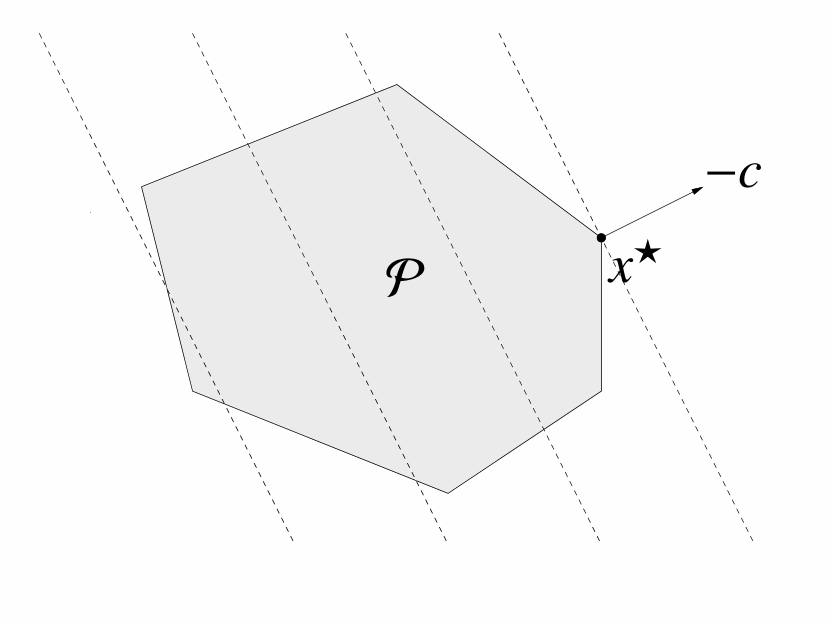
\includegraphics[width=0.75\linewidth]{img//marcoTeorico/optimizacion_fig2.png}
    \caption{Representación bidimensional de un conjunto de restricciones lineales (líneas rectas) que definen una región poliédrica sombreada correspondiente al conjunto factible de un problema de programación lineal (LP). Se ilustran además los contornos paralelos de la función objetivo lineal y la dirección de optimización. Adaptada de~\cite[p.~101]{BoydVandenbergheSlides2023}}%
    \label{fig:optimization2}
\end{figure}

Este enfoque es fundamental para algoritmos que iterativamente refinan una región de búsqueda. Utilizan los hiperplanos
generados por el oráculo para ``cortar'' o eliminar porciones del espacio de búsqueda que se sabe que no contienen
soluciones factibles, hasta que se encuentra una solución o se demuestra que la región de soluciones ``buenas'' (si existen)
es demasiado pequeña para ser relevante (de radio menor que $r$)~\cite[pp.~1, 5]{Sidford2020}.

Los problemas de factibilidad son cruciales en diversas áreas. Por ejemplo, en la minimización de funciones, muchos
algoritmos de optimización, especialmente los métodos de punto interior, requieren un punto inicial factible (o incluso
estrictamente factible) para comenzar~\cite[p.~579]{BoydVandenberghe2004},~\cite[p.~372]{BoydVandenbergheSlides2023}.
Determinar la existencia de tal punto es en sí mismo un problema de factibilidad. También surgen intrínsecamente en el
estudio de oráculos de separación para conjuntos y funciones convexas, que son componentes básicos de muchos algoritmos
de optimización eficientes~\cite[p.~1]{Sidford2020}.

%% Subsección: Relación y Contención
\subsection{Relación y Contención}\label{sec:relation_containment}

La relación entre los problemas de factibilidad y optimización es intrínseca y fundamental. Todo problema de optimización
inherentemente contiene un problema de factibilidad subyacente: antes de poder encontrar la ``mejor'' solución (óptima),
primero se debe determinar si existe \textit{alguna} solución que satisfaga todas las restricciones impuestas. Si el
conjunto factible es vacío, el problema de optimización es infactible y, por lo tanto, no tiene solución~\cite[p.~128]{BoydVandenberghe2004},~\cite[p.~90]{BoydVandenbergheSlides2023}.

Más formalmente, un \textbf{problema de factibilidad puede ser considerado un caso particular de un problema de optimización}~\cite[p.~130]{BoydVandenberghe2004},~\cite[p.~94]{BoydVandenbergheSlides2023}. Esto se logra simplemente definiendo una
función objetivo constante, por ejemplo, $f_0(x) = 0$ para todo $x$ (o cualquier otra constante). En este caso, el objetivo
de ``minimizar'' $f_0(x)$ se satisface trivialmente para cualquier $x$. Por lo tanto, cualquier punto factible $x$ es también
un punto óptimo, y el valor óptimo $p^*$ será $0$ si el problema es factible (es decir, si el conjunto factible no es vacío).
Si el problema es infactible, el valor óptimo $p^*$ será $\infty$ (asumiendo la convención de que el ínfimo de una función
sobre un conjunto vacío es $\infty$)~\cite[p.~129]{BoydVandenberghe2004},~\cite[p.~94]{BoydVandenbergheSlides2023}.

\begin{figure}
    \centering
    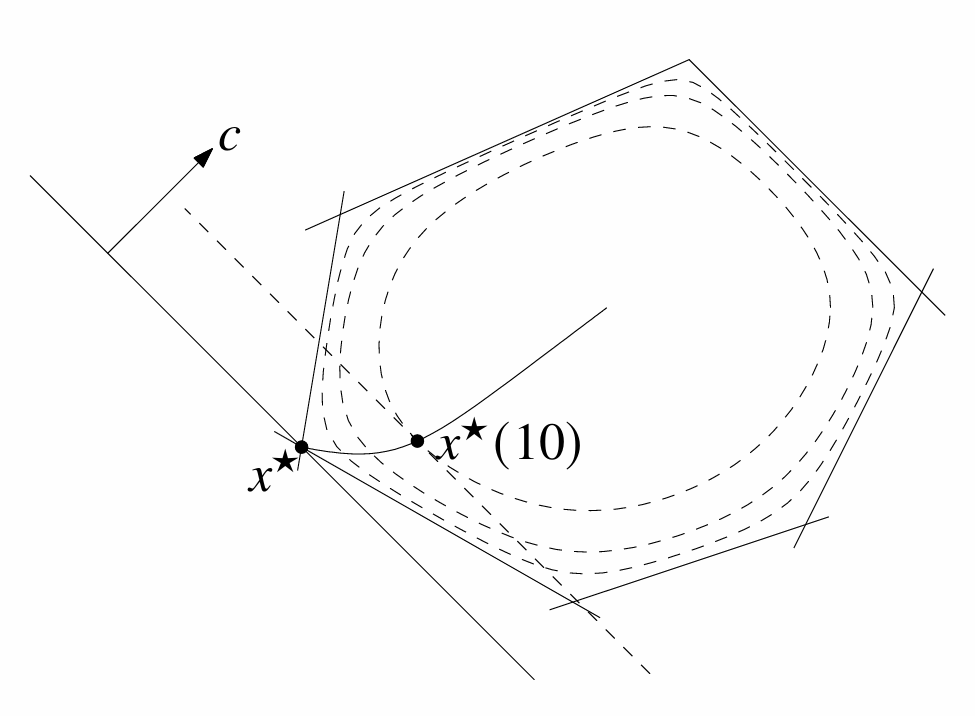
\includegraphics[width=0.75\linewidth]{img//marcoTeorico/optimizacion_fig3.png}
    \caption{Representación bidimensional del conjunto factible, el punto óptimo y la trayectoria central \( x^*(t) \) seguida por los métodos de barrera conforme el parámetro \( t \) incrementa. Se incluyen curvas de nivel que ilustran la función de barrera o, alternativamente, la función objetivo. Adaptada de~\cite[p.~361]{BoydVandenbergheSlides2023}}%
    \label{fig:optimization3}
\end{figure}

Esta contención es a menudo explotada en la práctica algorítmica. Por ejemplo, muchos métodos eficientes para resolver
problemas de optimización con restricciones de desigualdad, como los \textbf{métodos de barrera} (una clase importante
de \textbf{métodos de punto interior}\footnote{\textbf{Métodos de punto interior (\textit{Interior-point methods}):}
Una clase de algoritmos para resolver problemas de optimización lineal y no lineal convexa. A diferencia de los métodos
como el simplex que se mueven a lo largo de los bordes del conjunto factible, los métodos de punto interior generan una
secuencia de puntos estrictamente factibles en el \textit{interior} de la región factible que convergen al óptimo. A menudo
siguen una ``trayectoria central'' teórica, que es el conjunto de soluciones a una familia parametrizada de problemas de
optimización que incorporan una función de barrera (típicamente logarítmica) para las restricciones de desigualdad~\cite[Cap.~11]{BoydVandenberghe2004},~\cite[Cap.~9 y 11]{BoydVandenbergheSlides2023}.}), requieren un punto inicial
estrictamente factible (un punto $x$ tal que $f_i(x) < 0$ para todas las restricciones de desigualdad)~\cite[pp.~561, 568]{BoydVandenberghe2004},~\cite[pp.~355, 367]{BoydVandenbergheSlides2023}.

Si tal punto no se conoce de antemano, se emplea comúnmente un procedimiento de dos fases. La \textbf{fase I} consiste
en formular y resolver un problema de optimización auxiliar cuyo objetivo principal es encontrar un punto estrictamente
factible para el problema original. Si la fase I tiene éxito (es decir, encuentra un punto estrictamente factible), su
solución se utiliza como punto de partida para la \textbf{fase II}, que consiste en resolver el problema de optimización
original~\cite[p.~579]{BoydVandenberghe2004},~\cite[p.~372]{BoydVandenbergheSlides2023}. Una formulación común del
problema de fase I implica introducir una variable artificial $s$ y minimizar $s$ sujeto a las restricciones originales
modificadas, como $f_i(x) \leq s$. Este problema de fase I es en sí mismo un problema de optimización (a menudo convexo
si el original lo es) que busca determinar la factibilidad del problema original y encontrar un punto factible si existe~\cite[p.~579]{BoydVandenberghe2004},~\cite[p.~373]{BoydVandenbergheSlides2023}.\ \textit{[Aquí podría insertarse una
figura conceptual del método de barrera y la trayectoria central, como la Figura 11.2 de~\cite[p.~565]{BoydVandenberghe2004}
o la Figura 9.1 de~\cite[p.~361]{BoydVandenbergheSlides2023}, para ilustrar cómo, una vez asegurada la factibilidad
(a través de la fase I o por conocimiento previo), el algoritmo procede hacia la optimalidad manteniéndose dentro de la
región factible.]}

En resumen, la determinación de la factibilidad es un prerrequisito lógico y a menudo algorítmico para la optimización.
Un problema de optimización busca el ``mejor'' punto dentro del conjunto factible, mientras que un problema de factibilidad
simplemente busca determinar si dicho conjunto no está vacío y, en caso afirmativo, encontrar cualquier punto en él.
La capacidad de enmarcar problemas de factibilidad como problemas de optimización (con una función objetivo constante)
permite aplicar el amplio espectro de teorías y herramientas algorítmicas desarrolladas para la optimización también a la
resolución de problemas de factibilidad.
    \section[AGs Simples mediante \texttt{pymoo}]{Algoritmos Genéticos (AGs) Simples Mono-objetivo mediante \texttt{pymoo}}

\subsection{Introducción a los Algoritmos Genéticos (AGs) Simples}
La optimización, como disciplina fundamental, se dedica a la búsqueda de la mejor solución posible para un problema dado, considerando las restricciones existentes. Su importancia se manifiesta en una amplia gama de campos, desde la ingeniería y la ciencia hasta la economía y la inteligencia artificial, donde la necesidad de encontrar soluciones eficientes y efectivas es primordial. Dentro del vasto panorama de las técnicas de optimización, la computación evolutiva emerge como un paradigma de resolución de problemas inspirado en los mecanismos de la evolución natural~\cite{eiben2015}. Los Algoritmos Genéticos (AGs) constituyen una clase prominente de algoritmos evolutivos que han demostrado su eficacia en la resolución de problemas de optimización complejos~\cite{goldberg1989}.

La idea central detrás de los AGs radica en la simulación de los principios de la selección natural, la recombinación genética (cruce) y la mutación para mejorar iterativamente una población de soluciones candidatas~\cite{goldberg1989}. De manera análoga a la evolución biológica, donde los individuos mejor adaptados tienen una mayor probabilidad de sobrevivir y reproducirse, los AGs evalúan la ``aptitud'' de cada solución candidata mediante una función objetivo. Las soluciones más aptas tienen una mayor probabilidad de ser seleccionadas para producir la siguiente generación, combinando su información genética a través del cruce y sufriendo mutaciones aleatorias. Este proceso iterativo, que se repite a lo largo de varias generaciones, busca converger hacia una solución óptima para el problema planteado. El presente informe se centra específicamente en la implementación canónica de AGs simples diseñados para abordar problemas de optimización con un único objetivo dentro del contexto de la biblioteca Pymoo~\cite{blank2020}.

Los AGs resultan particularmente útiles para problemas de optimización mono-objetivo que presentan características desafiantes para los métodos tradicionales basados en gradientes. Su capacidad para explorar espacios de búsqueda complejos, no lineales y no diferenciables los convierte en una herramienta valiosa en escenarios donde la función objetivo exhibe múltiples óptimos locales o una superficie de búsqueda irregular. A diferencia de los métodos deterministas que siguen una trayectoria específica guiada por el gradiente, los AGs operan sobre una población de soluciones y emplean operadores estocásticos, lo que les permite explorar una gama más amplia de posibles soluciones y ser más robustos frente a quedar atrapados en óptimos locales. Esta característica fundamental motiva su aplicación en una variedad de problemas del mundo real donde la complejidad de la función objetivo dificulta el uso de técnicas convencionales.

El término ``canónico'' alude a una forma estándar o ampliamente aceptada del AG simple~\cite{goldberg1989}. Esta forma fundamental típicamente involucra la representación binaria de las soluciones candidatas, un mecanismo de selección proporcional a la aptitud (como la ruleta), un operador de cruce de un solo punto y un operador de mutación de inversión de bits. Si bien la biblioteca Pymoo puede ofrecer una mayor flexibilidad y una variedad de operadores más avanzados~\cite{blank2020}, comprender esta estructura básica es esencial para contextualizar la implementación específica que se analizará en este informe. Establecer esta base desde el principio permitirá al lector comprender mejor cómo la implementación de Pymoo se alinea con los principios fundamentales de un AG canónico y cómo potencialmente los extiende o adapta.

\subsection{Descripción General de la Biblioteca Pymoo}

Pymoo se presenta como una biblioteca moderna y rica en funcionalidades, escrita en Python y diseñada principalmente para abordar problemas de optimización multiobjetivo~\cite{blank2020}. No obstante, su arquitectura versátil y su diseño modular la convierten también en una herramienta poderosa para la resolución de problemas de optimización con un único objetivo. Una de sus principales fortalezas reside en su capacidad para separar claramente los componentes de un problema de optimización (la función objetivo, las variables de decisión y las restricciones) de los algoritmos de optimización propiamente dichos y de los operadores genéticos utilizados. Esta separación promueve la flexibilidad y la reutilización del código, permitiendo a los usuarios experimentar fácilmente con diferentes combinaciones de algoritmos y operadores para un mismo problema.

La biblioteca Pymoo destaca por su amplio soporte para una variedad de algoritmos de optimización, que abarcan tanto técnicas evolutivas, como los Algoritmos Genéticos, la Optimización por Enjambre de Partículas y la Evolución Diferencial, como también métodos clásicos de optimización~\cite{blank2020}. Además, proporciona un conjunto completo de herramientas para la definición de problemas de optimización, la implementación de operadores genéticos personalizados y la evaluación del rendimiento de los algoritmos. Su extensibilidad es otra característica clave, ya que permite a los usuarios implementar fácilmente sus propios algoritmos, operadores o criterios de terminación si las opciones predefinidas no se ajustan a sus necesidades específicas.

Aunque el enfoque principal de Pymoo radica en la optimización multiobjetivo~\cite{Deb2005, blank2020}, su marco de trabajo subyacente y muchos de sus operadores pueden aplicarse directamente o tienen contrapartidas específicas para el caso de la optimización con un solo objetivo. Esto significa que los usuarios interesados en resolver problemas con una única función objetivo pueden beneficiarse igualmente de la robustez y la flexibilidad que ofrece la biblioteca. La arquitectura de Pymoo se organiza en varios módulos clave que interactúan para definir y ejecutar los procesos de optimización. Estos módulos incluyen:
\begin{itemize}
    \item \texttt{\seqsplit{pymoo.core.problem}}: Este módulo proporciona las clases base para definir problemas de optimización, especificando la función objetivo, el número y los límites de las variables de decisión, así como cualquier restricción que deba cumplirse.
    \item \texttt{\seqsplit{pymoo.algorithms}}: Contiene implementaciones de una amplia gama de algoritmos de optimización, incluyendo la clase GA para problemas mono-objetivo que será el foco de este informe.
    \item \texttt{\seqsplit{pymoo.operators}}: Ofrece una colección diversa de operadores genéticos esenciales para los algoritmos evolutivos, como operadores de selección (para elegir los padres), operadores de cruce (para combinar la información genética) y operadores de mutación (para introducir variaciones aleatorias).
    \item \texttt{\seqsplit{pymoo.termination}}: Define diferentes criterios que pueden utilizarse para detener el proceso de optimización, como alcanzar un número máximo de generaciones o un cierto nivel de convergencia.
    \item \texttt{\seqsplit{pymoo.optimize}}: Proporciona funciones de alto nivel para facilitar la ejecución de los algoritmos de optimización una vez que se han definido el problema y el algoritmo deseado.
\end{itemize}

La filosofía de diseño de Pymoo, que separa claramente la definición del problema, la implementación del algoritmo y la aplicación de los operadores, promueve una flexibilidad y una capacidad de reutilización significativas~\cite{blank2020}. Esto implica que un mismo problema de optimización podría potencialmente resolverse utilizando diferentes algoritmos mono-objetivo disponibles en Pymoo, lo que facilita la realización de estudios comparativos de rendimiento. Esta capacidad de desacoplamiento permite a los usuarios experimentar con diversas combinaciones de algoritmos y operadores sin necesidad de reescribir la definición del problema cada vez, lo que representa una ventaja considerable tanto para la investigación como para las aplicaciones prácticas.

\subsection{El Algoritmo Genético Canónico en Pymoo}

Pymoo proporciona una implementación fácilmente accesible de un Algoritmo Genético mono-objetivo que se alinea de cerca con la forma canónica descrita anteriormente~\cite{goldberg1989}. Dentro de la biblioteca, la clase \texttt{\seqsplit{pymoo.algorithms.soo.nonconvex.ga.GA}}, ubicada en el módulo \texttt{\seqsplit{pymoo.algorithms.soo.nonconvex}}, constituye el foco principal para la discusión de la implementación canónica de un AG mono-objetivo~\cite{blank2020}. La designación \texttt{\seqsplit{soo}} en el nombre del módulo indica que se trata de un algoritmo diseñado para la Optimización con un Solo Objetivo, mientras que \texttt{\seqsplit{nonconvex}} sugiere que es adecuado para problemas donde la función objetivo puede no ser convexa, una característica común en los escenarios donde los AGs suelen ser efectivos.

Si bien Pymoo ofrece una variedad de otros algoritmos de optimización mono-objetivo, la clase \texttt{\seqsplit{GA}} se destaca como una representación directa de un AG estándar, incorporando los componentes fundamentales y el flujo de trabajo típico de este tipo de algoritmo evolutivo. El proceso general para utilizar la clase \texttt{\seqsplit{GA}} en Pymoo sigue una serie de pasos bien definidos:
\begin{itemize}
    \item \textbf{Definición del Problema de Optimización:} El primer paso crucial consiste en definir el problema específico que se desea resolver. Esto se realiza mediante la creación de una instancia de la clase \texttt{\seqsplit{Problem}} de Pymoo (o una de sus subclases), donde se especifica la función objetivo que se va a minimizar o maximizar, el número de variables de decisión involucradas y los límites inferior y superior para cada una de estas variables. Adicionalmente, si el problema incluye alguna restricción que las soluciones deben satisfacer, estas también se definen en este paso.
    \item \textbf{Creación de una Instancia del Algoritmo Genético:} Una vez definido el problema, se procede a crear una instancia de la clase \texttt{\seqsplit{GA}}. Durante esta instanciación, se deben especificar varios parámetros que controlan el comportamiento del algoritmo, como el tamaño de la población (\texttt{\seqsplit{pop\_size}}), el método de muestreo para generar la población inicial (\texttt{\seqsplit{sampling}}), el operador de cruce (\texttt{\seqsplit{crossover}}) que se utilizará para combinar la información genética de los padres y el operador de mutación (\texttt{\seqsplit{mutation}}) que se aplicará para introducir variaciones aleatorias en la descendencia.
    \item \textbf{Ejecución del Algoritmo:} Con el problema definido y el algoritmo instanciado y configurado, el siguiente paso es ejecutar el proceso de optimización. Esto se logra llamando al método \texttt{\seqsplit{solve~()}} de la instancia de la clase \texttt{\seqsplit{GA}}, pasando como argumento el objeto que representa el problema de optimización definido en el paso anterior.
    \item \textbf{Análisis de los Resultados:} Una vez que el algoritmo ha terminado de ejecutarse (ya sea por alcanzar un criterio de terminación predefinido o por completarse el número máximo de generaciones), el método \texttt{\seqsplit{solve~()}} devuelve un objeto de tipo \texttt{\seqsplit{Result}} que contiene información relevante sobre la ejecución de la optimización. Esta información típicamente incluye la mejor solución encontrada (los valores de las variables de decisión que producen el mejor valor de la función objetivo) y el valor correspondiente de la función objetivo.
\end{itemize}

Es importante señalar que, si bien la clase \texttt{\seqsplit{pymoo.algorithms.soo.nonconvex.ga.GA}} es una representación fundamental de un AG canónico dentro de Pymoo~\cite{blank2020}, la flexibilidad de la biblioteca podría permitir la existencia de otras implementaciones o variantes de AGs, ya sea dentro de la propia biblioteca o aportadas por la comunidad de usuarios. No obstante, para los fines de este informe y con el objetivo de proporcionar una comprensión clara de la forma ``canónica'', nos centraremos en el análisis detallado de esta clase específica debido a su estrecha correspondencia con la estructura tradicional de un AG~\cite{goldberg1989}.

\subsection{Análisis Detallado de la Clase \texttt{\url{pymoo.algorithms.soo.nonconvex.ga.GA}}}

La clase \texttt{\seqsplit{pymoo.algorithms.soo.nonconvex.ga.GA}} se configura principalmente a través de su constructor, que acepta varios parámetros clave que definen el comportamiento del algoritmo genético. Estos parámetros permiten a los usuarios adaptar el algoritmo a las características específicas del problema que se está abordando. A continuación, se presenta un análisis detallado de los parámetros más importantes del constructor:
\begin{itemize}
    \item \texttt{\seqsplit{pop\_size}}: Este parámetro de tipo entero especifica el número de individuos que conformarán la población en cada generación del algoritmo. El tamaño de la población influye significativamente en el rendimiento del AG.\ Una población más grande permite una mayor exploración del espacio de búsqueda, lo que puede aumentar la probabilidad de encontrar la solución óptima, pero también incrementa el costo computacional. Por otro lado, una población más pequeña puede converger más rápidamente, pero corre el riesgo de quedar atrapada en óptimos locales. La elección del tamaño de la población suele ser un compromiso que depende de la complejidad del problema y los recursos computacionales disponibles.
    \item \texttt{\seqsplit{sampling}}: Este parámetro define el método que se utilizará para crear la población inicial de individuos. Acepta un objeto de una clase de muestreo proporcionada por Pymoo (generalmente del módulo \texttt{\seqsplit{pymoo.operators.sampling}}). Una opción común es \texttt{\seqsplit{RandomSampling}}, que genera individuos con valores de variables de decisión distribuidos uniformemente dentro de sus respectivos límites. La estrategia de muestreo inicial puede tener un impacto considerable en la diversidad inicial de la población, lo que a su vez puede afectar la capacidad del algoritmo para explorar eficazmente el espacio de búsqueda.
    \item \texttt{\seqsplit{crossover}}: Este parámetro especifica el operador de cruce que se aplicará durante el proceso de reproducción. Acepta un objeto de una clase de operador de cruce del módulo \texttt{\seqsplit{pymoo.operators.crossover}}. Pymoo ofrece una variedad de operadores de cruce diseñados para diferentes tipos de representación de variables de decisión. Por ejemplo, para problemas con variables continuas, un operador común es \texttt{\seqsplit{SBX}} (Simulated Binary Crossover)~\cite{deb1995}, mientras que para problemas con variables binarias se podrían utilizar operadores como \texttt{\seqsplit{SinglePointCrossover}} o \texttt{\seqsplit{TwoPointCrossover}}. La elección del operador de cruce influye en cómo se combina la información genética de los padres para generar nuevos descendientes.
    \item \texttt{\seqsplit{mutation}}: De manera similar al parámetro \texttt{\seqsplit{crossover}}, este parámetro define el operador de mutación que se utilizará para introducir variaciones aleatorias en la población. Acepta un objeto de una clase de operador de mutación del módulo \texttt{\seqsplit{pymoo.operators.mutation}}. Al igual que con el cruce, Pymoo proporciona varios operadores de mutación adecuados para diferentes tipos de variables. Por ejemplo, \texttt{\seqsplit{PolynomialMutation}} se utiliza a menudo para variables continuas~\cite{deb1996}, mientras que \texttt{\seqsplit{BitflipMutation}} es común para variables binarias. El operador de mutación juega un papel crucial en el mantenimiento de la diversidad genética y en la prevención de la convergencia prematura del algoritmo.
    \item \texttt{\seqsplit{eliminate\_duplicates}}: Este parámetro booleano indica si se deben eliminar los individuos duplicados de la población después de cada generación. Si se establece en \texttt{\seqsplit{True}}, el algoritmo verificará si existen individuos idénticos en la nueva población y los eliminará, manteniendo así una mayor diversidad genética. Si se establece en \texttt{\seqsplit{False}}, se permitirán los duplicados. La eliminación de duplicados puede ayudar a prevenir la convergencia prematura, pero también puede añadir una sobrecarga computacional al proceso.
\end{itemize}

La principal funcionalidad de la clase \texttt{\seqsplit{GA}} se expone a través de sus métodos, siendo el más importante de ellos el método \texttt{\seqsplit{solve~()}}. Este método es el encargado de ejecutar el algoritmo genético y llevar a cabo el proceso iterativo de evolución de la población hasta que se cumple algún criterio de terminación. El método \texttt{\seqsplit{solve~()}} requiere como entrada principal un objeto que represente el problema de optimización que se desea resolver. Este objeto debe ser una instancia de una subclase de \texttt{\seqsplit{pymoo.core.problem.Problem}} y debe definir la función objetivo, el número y los límites de las variables de decisión, y cualquier restricción que sea aplicable. La separación entre la definición del problema y la implementación del algoritmo es un aspecto fundamental del diseño de Pymoo, ya que permite una mayor flexibilidad y modularidad en el proceso de optimización~\cite{blank2020}.

Al finalizar su ejecución, el método \texttt{\seqsplit{solve~()}} devuelve un objeto de tipo \texttt{\seqsplit{pymoo.optimize.result.Result}}. Este objeto contiene información valiosa sobre la ejecución del algoritmo, incluyendo el mejor individuo encontrado durante todo el proceso de optimización (accesible a través del atributo \texttt{\seqsplit{X}}) y el valor correspondiente de la función objetivo para ese individuo (accesible a través del atributo \texttt{\seqsplit{F}}). Además de la mejor solución, el objeto \texttt{\seqsplit{Result}} puede contener otra información útil, como el historial de la evolución de la población o métricas de rendimiento del algoritmo.

\subsection{Componentes y Operadores Clave}
\begin{itemize}[label=\textbullet, leftmargin=*]
    \item \textbf{Inicialización:} La primera etapa en la ejecución de un Algoritmo Genético es la creación de la población inicial de soluciones candidatas. En Pymoo, este proceso está determinado por el parámetro \texttt{\seqsplit{sampling}} que se especifica al instanciar la clase \texttt{\seqsplit{GA}}. El método de muestreo elegido define cómo se generan los individuos iniciales en el espacio de búsqueda del problema. Una estrategia común es \texttt{\seqsplit{RandomSampling}}, que genera soluciones distribuidas uniformemente dentro de los límites definidos para cada variable de decisión. Otras estrategias de muestreo, como el muestreo de hipercubo latino (LHS), también podrían estar disponibles en Pymoo y ofrecer diferentes formas de distribuir inicialmente las soluciones en el espacio de búsqueda. La diversidad de la población inicial es un factor crítico que puede influir significativamente en la capacidad del AG para encontrar el óptimo global. Una población inicial bien diversificada aumenta las posibilidades de explorar una región más amplia del espacio de búsqueda y de evitar la convergencia prematura hacia óptimos locales. La elección de una estrategia de muestreo apropiada debe basarse en las características del problema específico que se está abordando.

    \item \textbf{Evaluación:} Una vez que se ha generado la población inicial (y en cada generación subsiguiente), es necesario evaluar la calidad de cada individuo, es decir, qué tan bien resuelve el problema de optimización. En Pymoo, esta evaluación se realiza llamando a la función objetivo definida dentro del objeto \texttt{\seqsplit{Problem}} para cada individuo de la población. El valor resultante de la función objetivo (o valores, en el caso de optimización multiobjetivo, aunque aquí nos centramos en el caso mono-objetivo) representa la aptitud o ``fitness'' de ese individuo. Cuanto mejor sea el valor de la función objetivo (dependiendo de si se busca minimizar o maximizar), mayor será la aptitud del individuo.

    \item \textbf{Selección:} El operador de selección juega un papel fundamental en la evolución de la población al determinar qué individuos de la generación actual se elegirán como padres para producir la siguiente generación. El objetivo de la selección es favorecer a los individuos con mayor aptitud, aumentando así la probabilidad de que sus ``genes'' (es decir, sus características como soluciones) se transmitan a la siguiente generación. Pymoo implementa varios métodos de selección comunes~\cite{goldberg1989, eiben2015}:
    \begin{itemize}[label=\textbullet, leftmargin=*] % Cambiado a \textbullet
        \item \textit{Selección por Torneo:} En este método, se selecciona aleatoriamente un pequeño grupo de individuos (el tamaño del torneo es un parámetro configurable). El individuo con la mejor aptitud dentro de este grupo se elige como padre. Este proceso se repite hasta que se ha seleccionado el número deseado de padres. El tamaño del torneo influye en la presión de selección: un tamaño mayor aumenta la probabilidad de que los individuos más aptos sean seleccionados.
        \item \textit{Selección por Ruleta (Selección Proporcional a la Aptitud):} En este método, a cada individuo se le asigna una probabilidad de ser seleccionado proporcional a su aptitud relativa en la población. Los individuos con mayor aptitud tienen una mayor probabilidad de ser elegidos. Sin embargo, este método puede presentar problemas si hay un individuo excepcionalmente apto en las primeras generaciones, ya que podría dominar el proceso de selección y llevar a una convergencia prematura.
        \item Pymoo podría ofrecer otros métodos de selección, como la selección basada en el rango, donde la probabilidad de selección se basa en el rango de aptitud del individuo en lugar de su valor absoluto. La elección del método de selección y sus parámetros asociados tiene un impacto significativo en la velocidad de convergencia y en el riesgo de convergencia prematura del algoritmo. Una mayor presión de selección puede acelerar la convergencia, pero también puede aumentar el riesgo de quedar atrapado en óptimos locales.
    \end{itemize}

    \item \textbf{Cruce (Recombinación):} El operador de cruce, también conocido como recombinación, es un mecanismo clave en los Algoritmos Genéticos que permite combinar la información genética de dos individuos padres seleccionados para crear nuevos individuos descendientes~\cite{goldberg1989}. El objetivo del cruce es explorar nuevas regiones del espacio de búsqueda mediante la creación de combinaciones de características que podrían no existir en los padres individualmente. Pymoo proporciona una variedad de operadores de cruce, algunos de los cuales son:
    \begin{itemize}[label=\textbullet, leftmargin=*] % Cambiado a \textbullet
        \item \textit{Cruce de un Punto:} Para representaciones binarias o de enteros, se elige aleatoriamente un único punto de cruce. Los segmentos de los cromosomas de los dos padres se intercambian en este punto para producir dos nuevos descendientes.
        \item \textit{Cruce de Dos Puntos:} Similar al cruce de un punto, pero se eligen dos puntos de cruce. El segmento del cromosoma entre estos dos puntos se intercambia entre los dos padres.
        \item \textit{Cruce Binario Simulado (SBX):} Este operador se utiliza comúnmente para problemas con variables continuas~\cite{deb1995}. Simula el comportamiento del cruce de un punto en el espacio de las variables reales, generando descendientes que se encuentran en la vecindad de los padres en el espacio de búsqueda. El \texttt{\seqsplit{SBX}} tiene un parámetro importante, el factor de dispersión, que controla qué tan lejos de los padres pueden estar los descendientes.
        \item Pymoo puede incluir otros operadores de cruce, como el cruce uniforme, donde cada gen (variable) del descendiente se selecciona aleatoriamente de uno de los dos padres. La elección del operador de cruce debe ser compatible con la representación de las soluciones (por ejemplo, binaria, continua) y puede tener un impacto significativo en la capacidad del algoritmo para explorar y explotar el espacio de búsqueda. El operador de cruce y sus parámetros se especifican en Pymoo a través del parámetro \texttt{\seqsplit{crossover}} en el constructor de la clase \texttt{\seqsplit{GA}}.
    \end{itemize}

    \item \textbf{Mutación:} El operador de mutación introduce pequeños cambios aleatorios en los individuos descendientes después del cruce. El propósito de la mutación es mantener la diversidad genética en la población y evitar la convergencia prematura hacia un óptimo local al introducir nuevo material genético que no estaba presente en la población de padres~\cite{goldberg1989, eiben2015}. Pymoo ofrece varios operadores de mutación:
    \begin{itemize}[label=\textbullet, leftmargin=*] % Cambiado a \textbullet
        \item \textit{Mutación por Inversión de Bits:} Este operador se aplica típicamente a representaciones binarias. Para cada bit del cromosoma de un individuo, existe una pequeña probabilidad (la tasa de mutación) de que su valor se invierta (de 0 a 1 o de 1 a 0).
        \item \textit{Mutación Polinomial:} Este operador se utiliza a menudo para problemas con variables continuas~\cite{deb1996}. Perturba el valor de cada variable de decisión en un individuo en función de una distribución polinomial. La magnitud de la perturbación está controlada por parámetros como la tasa de mutación y el índice de distribución.
        \item Pymoo puede proporcionar otros operadores de mutación, como la mutación gaussiana para variables continuas, donde se añade un pequeño valor aleatorio extraído de una distribución gaussiana al valor de la variable. La tasa de mutación es un parámetro crítico. Una tasa demasiado baja podría no introducir suficiente diversidad, mientras que una tasa demasiado alta podría perturbar las buenas soluciones y hacer que la búsqueda sea más aleatoria. El operador de mutación y sus parámetros se especifican en Pymoo mediante el parámetro \texttt{\seqsplit{mutation}} en el constructor de la clase \texttt{\seqsplit{GA}}.
    \end{itemize}

    \item \textbf{Reemplazo:} Después de que se han generado los nuevos individuos descendientes a través de los procesos de selección, cruce y mutación, es necesario determinar cómo se formará la siguiente generación de la población. En un Algoritmo Genético simple, la estrategia de reemplazo más común es reemplazar toda la población de padres por la población de hijos. Sin embargo, Pymoo podría ofrecer opciones para implementar el elitismo, una estrategia donde uno o varios de los mejores individuos de la generación anterior se conservan y se pasan directamente a la siguiente generación, asegurando que las mejores soluciones encontradas hasta el momento no se pierdan. La implementación del elitismo puede mejorar el rendimiento y la fiabilidad del AG al garantizar que el progreso realizado durante la optimización se mantenga.

    \item \textbf{Criterios de Terminación:} Es fundamental definir cuándo debe detenerse el proceso iterativo del Algoritmo Genético. Sin criterios de terminación adecuados, el algoritmo podría ejecutarse indefinidamente. Pymoo proporciona varios criterios de terminación comunes que se pueden utilizar:
    \begin{itemize}[label=\textbullet, leftmargin=*] % Cambiado a \textbullet
        \item \textit{Número Máximo de Generaciones:} El algoritmo se detiene después de que se ha alcanzado un número predefinido de generaciones. Este es un criterio de terminación simple y comúnmente utilizado.
        \item \textit{Número Máximo de Evaluaciones de la Función Objetivo:} El algoritmo se detiene después de que la función objetivo ha sido evaluada un número máximo de veces. Este criterio es útil en problemas donde la evaluación de la función objetivo es computacionalmente costosa.
        \item \textit{Tolerancia en la Convergencia:} El algoritmo se detiene cuando la mejora en el valor de la función objetivo entre generaciones sucesivas es menor que un umbral predefinido durante un cierto número de generaciones. Esto indica que el algoritmo ha convergido a una solución (posiblemente local).
        \item Pymoo puede ofrecer otros criterios de terminación, como un tiempo máximo de ejecución. Los criterios de terminación se suelen especificar al llamar al método \texttt{\seqsplit{solve~()}} de la clase \texttt{\seqsplit{GA}} o mediante el uso de objetos específicos de criterios de terminación del módulo \texttt{\seqsplit{pymoo.termination}}. La elección de los criterios de terminación adecuados es crucial para asegurar que el algoritmo se ejecute durante el tiempo suficiente para encontrar una buena solución sin desperdiciar recursos computacionales.
    \end{itemize}
\end{itemize}

\subsection{Implementación y Uso Práctico}

A continuación, se presenta un ejemplo de código conciso que ilustra cómo utilizar la clase \texttt{\seqsplit{pymoo.algorithms.soo.nonconvex.ga.GA}} de Pymoo para resolver un problema simple de optimización mono-objetivo. Este ejemplo demostrará los pasos esenciales para definir el problema, configurar el algoritmo genético, ejecutar la optimización y analizar los resultados.
\newpage
\begin{listing}[H]
\begin{minted}[linenos, breaklines]{python}
import numpy as np
from pymoo.core.problem import Problem
from pymoo.algorithms.soo.nonconvex.ga import GA
from pymoo.operators.sampling.rnd import RandomSampling
from pymoo.operators.crossover.sbx import SBX
from pymoo.operators.mutation.pm import PolynomialMutation
from pymoo.optimize import minimize

# 1. Definir el problema de optimización
class MyProblem(Problem):
    def __init__(self):
        super().__init__(n_var=2, n_obj=1, n_constr=0, xl=-5, xu=5)

    def _evaluate(self, x, out, *args, **kwargs):
        out["F"] = np.sum(x**2, axis=1)

# 2. Crear una instancia del problema
problem = MyProblem()

# 3. Crear una instancia del algoritmo genético
algorithm = GA(pop_size=20, sampling=RandomSampling(), crossover=SBX(prob=0.9, eta=15), mutation=PolynomialMutation(prob=0.1, eta=20),eliminate_duplicates=True)

# 4. Ejecutar el algoritmo de optimización
res = minimize(problem,algorithm, ("n_gen", 100), verbose=False)

# 5. Analizar los resultados
print("Mejor solución encontrada:", res.X)
print("Valor de la función objetivo para la mejor solución:", res.F)
\end{minted}
\caption{Ejemplo de código Pymoo para optimización mono-objetivo con AG}
\label{lst:pymoo_example}
\end{listing}



En este ejemplo, primero se define un problema de optimización simple (\texttt{\seqsplit{MyProblem}}) donde el objetivo es minimizar la suma de los cuadrados de dos variables de decisión, cada una con límites entre -5 y 5. Luego, se crea una instancia de la clase \texttt{\seqsplit{GA}}, especificando un tamaño de población de 20 individuos, utilizando un muestreo aleatorio para la población inicial, el operador de cruce \texttt{\seqsplit{SBX}}~\cite{deb1995} con una probabilidad de 0.9 y un factor de distribución de 15, el operador de mutación polinomial~\cite{deb1996} con una probabilidad de 0.1 y un factor de distribución de 20, y habilitando la eliminación de duplicados. A continuación, se llama a la función \texttt{\seqsplit{minimize}} de Pymoo, que toma el problema, el algoritmo y un criterio de terminación (en este caso, un máximo de 100 generaciones) como argumentos. Finalmente, se imprimen la mejor solución encontrada (\texttt{\seqsplit{res.X}}) y el valor correspondiente de la función objetivo (\texttt{\seqsplit{res.F}}). Este ejemplo ilustra el flujo de trabajo básico para utilizar el AG canónico en Pymoo~\cite{blank2020}.

\subsubsection{Configuración y Ajuste de Parámetros}

La elección adecuada de los valores para los parámetros del Algoritmo Genético, como el tamaño de la población, la probabilidad de cruce y la probabilidad de mutación, es de suma importancia para lograr un buen rendimiento del algoritmo~\cite{eiben2015}. Estos parámetros influyen directamente en la capacidad del algoritmo para explorar el espacio de búsqueda, explotar las buenas soluciones encontradas y converger hacia un óptimo. No existe un conjunto de parámetros universalmente óptimo que funcione bien para todos los problemas; los mejores valores a menudo dependen de las características específicas del problema que se está resolviendo.

El tamaño de la población (\texttt{\seqsplit{pop\_size}}) determina el número de soluciones candidatas que se mantienen y evolucionan en cada generación. Un tamaño de población mayor permite una exploración más exhaustiva del espacio de búsqueda, lo que puede aumentar la probabilidad de encontrar el óptimo global, especialmente en problemas complejos con muchos óptimos locales. Sin embargo, una población más grande también implica un mayor costo computacional por generación. Por otro lado, un tamaño de población más pequeño puede resultar en una convergencia más rápida, pero corre el riesgo de estancarse en óptimos locales debido a una exploración limitada. Los rangos típicos para el tamaño de la población pueden variar ampliamente, desde unas pocas decenas hasta varios cientos, dependiendo de la complejidad del problema.

La probabilidad de cruce (a menudo un parámetro del operador de cruce, como \texttt{\seqsplit{prob}} en el ejemplo del operador \texttt{\seqsplit{SBX}}) controla la frecuencia con la que se aplica el operador de cruce a los padres seleccionados. Una probabilidad de cruce alta favorece la exploración al generar nuevas soluciones mediante la combinación de la información genética de los padres. Una probabilidad de cruce baja, por otro lado, permite que las soluciones se transmitan a la siguiente generación con menos cambios, lo que puede ser beneficioso en las etapas posteriores de la búsqueda cuando se están afinando las soluciones cercanas al óptimo. Los valores típicos para la probabilidad de cruce suelen estar en el rango de 0.8 a 0.95~\cite{eiben2015}.

La probabilidad o tasa de mutación (a menudo un parámetro del operador de mutación, como \texttt{\seqsplit{prob}} en el ejemplo del operador de mutación polinomial) determina la probabilidad de que cada gen (o variable) en un individuo descendiente se modifique aleatoriamente. La mutación juega un papel crucial en el mantenimiento de la diversidad genética y en la prevención de la convergencia prematura al introducir nuevas características en la población que no estaban presentes en los padres. Una tasa de mutación demasiado baja puede resultar en una falta de exploración de nuevas áreas del espacio de búsqueda, mientras que una tasa demasiado alta puede perturbar las buenas soluciones y hacer que la búsqueda sea esencialmente aleatoria. Los valores típicos para la tasa de mutación suelen ser bajos, a menudo en el rango de 0.01 a 0.1, dependiendo del problema y la representación~\cite{eiben2015}.

Dado que no existen reglas fijas para determinar los valores óptimos de estos parámetros, a menudo es necesario recurrir a la experimentación para encontrar una configuración que funcione bien para un problema específico. Esto puede implicar ejecutar el algoritmo con diferentes combinaciones de parámetros y comparar su rendimiento en términos de la calidad de la solución encontrada y la velocidad de convergencia. Algunas técnicas más avanzadas para el ajuste de parámetros incluyen la búsqueda en cuadrícula (grid search), la búsqueda aleatoria (random search) y métodos de control de parámetros adaptativos, donde los parámetros del algoritmo se ajustan dinámicamente durante el proceso de optimización en función de su rendimiento.

La siguiente tabla (Tabla~\ref{tab:ga_params}) resume los parámetros clave de la clase \texttt{\seqsplit{pymoo.algorithms.soo.nonconvex.ga.GA}} y su impacto en el rendimiento del algoritmo:

\begin{table}[htbp]
\centering
\caption{Parámetros Clave de la Clase \texttt{\url{pymoo.algorithms.soo.nonconvex.ga.GA}}}%
\label{tab:ga_params}
\begin{tabularx}{\textwidth}{@{}l>{\raggedright\arraybackslash}X>{\raggedright\arraybackslash}p{0.2\textwidth}>{\raggedright\arraybackslash}X@{}}
\toprule
\textbf{Parámetro} & \textbf{Descripción} & \textbf{Rango/Valores Típicos} & \textbf{Impacto en el Rendimiento} \\
\midrule
\texttt{\seqsplit{pop\_size}} & Número de individuos en la población. & 50\-500 (según la complejidad) & Valores más altos aumentan la exploración pero también el costo computacional. Valores más bajos pueden llevar a convergencia prematura. \\
\midrule
\texttt{\seqsplit{sampling}} & Método para crear la población inicial. & \texttt{\seqsplit{RandomSampling}}, \texttt{\seqsplit{LHS}} & Influye en la diversidad inicial de la población y la cobertura del espacio de búsqueda. \\
\midrule
\texttt{\seqsplit{crossover}} & Operador de cruce para generar descendencia (ej., \texttt{\seqsplit{SBX}}~\cite{deb1995}, \texttt{\seqsplit{PMX}}). & Depende del problema & Determina cómo se combina la información genética. Diferentes operadores tienen diferentes características de búsqueda. \\
\midrule
\texttt{\seqsplit{mutation}} & Operador de mutación para mantener diversidad (ej., \texttt{\seqsplit{PolynomialMutation}}~\cite{deb1996}). & Depende de la codificación & Introduce cambios aleatorios para mantener la diversidad genética y evitar óptimos locales. \\
\midrule
\texttt{\seqsplit{eliminate\_duplicates}} & Indicador para eliminar individuos duplicados. & \texttt{\seqsplit{True}}, \texttt{\seqsplit{False}} & Ayuda a prevenir convergencia prematura manteniendo diversidad, pero añade costo computacional. \\
\bottomrule
\end{tabularx}
\end{table}

\subsection{Consideraciones Adicionales}

La modularidad de Pymoo facilita la experimentación con diferentes componentes del AG, como los operadores de selección, cruce y mutación, lo que permite a los investigadores y profesionales explorar diversas estrategias evolutivas para encontrar soluciones óptimas. Si bien esta sección del marco teórico se ha centrado en la implementación canónica del AG, es importante destacar que Pymoo ofrece una amplia gama de otros algoritmos de optimización mono-objetivo, como la Evolución Diferencial y la Optimización por Enjambre de Partículas (PSO), que podrían ser explorados como alternativas o complementos al AG.\ Además, para problemas que involucran múltiples objetivos, Pymoo es especialmente potente gracias a su enfoque principal en la optimización multiobjetivo~\cite{Deb2005, blank2020}.

La extensibilidad de Pymoo permite a los usuarios avanzados implementar sus propios operadores genéticos o modificar el comportamiento del algoritmo \texttt{\seqsplit{GA}} existente para satisfacer necesidades específicas. Para aplicaciones del mundo real, es crucial considerar las posibles restricciones que pueden existir en el problema de optimización. Pymoo proporciona mecanismos para manejar restricciones en problemas mono-objetivo utilizando AGs, lo que amplía su aplicabilidad a una gama más amplia de escenarios. Finalmente, es fundamental evaluar el rendimiento del AG utilizando métricas apropiadas, como la velocidad de convergencia, la calidad de la solución obtenida y la robustez del algoritmo frente a diferentes ejecuciones.

Se anima a los usuarios a experimentar con la clase \texttt{\seqsplit{GA}} en Pymoo y a explorar la extensa documentación de la biblioteca~\cite{blank2020} para descubrir características más avanzadas y aplicaciones en diversos dominios de la optimización. La comprensión de los fundamentos del AG canónico proporcionados en este informe sirve como una base sólida para explorar las capacidades más amplias de Pymoo y para abordar una variedad de problemas de optimización complejos.

    \section[FrameworkQt \& PyQt]{Framework de interfaz: Qt \& PyQt}

\subsection{Introducción a Qt}
El framework Qt se define formalmente como un entorno de desarrollo de aplicaciones multiplataforma, diseñado para la creación de interfaces gráficas de usuario (GUI) y aplicaciones que pueden ejecutarse en diversos sistemas operativos y plataformas de hardware, incluyendo Linux, Windows, macOS, Android y sistemas embebidos, con mínimas o nulas modificaciones en el código subyacente~\cite{qt_wiki}. Constituye un conjunto integral de clases de biblioteca C++ altamente intuitivas y modularizadas, enriquecidas con APIs que simplifican el proceso de desarrollo de aplicaciones~\cite{qt_framework}. Esta capacidad permite a los programadores escribir código una sola vez y distribuirlo a través de múltiples plataformas, abarcando desde aplicaciones de escritorio hasta sistemas embebidos~\cite{businesscloud}. La cualidad de ser multiplataforma, a menudo resumida en el principio de ``escribir una vez, ejecutar en cualquier lugar'' (WORA, por sus siglas en inglés), representa una ventaja fundamental de Qt, ya que reduce significativamente los tiempos y costos de desarrollo al mismo tiempo que permite alcanzar una audiencia más amplia~\cite{lemberg}. Además, el hecho de que C++ sea el lenguaje subyacente~\cite{qt_wiki} sugiere un enfoque en el rendimiento y el acceso a funcionalidades de bajo nivel del sistema.

La historia de Qt se remonta a 1990, cuando los programadores noruegos Eirik Chambe-Eng y Haavard Nord concibieron la idea, con el primer lanzamiento público en 1995 para el sistema operativo Linux~\cite{qt_history}. Inicialmente fue desarrollado por la empresa Trolltech, que posteriormente fue adquirida por Nokia, luego por Digia y actualmente es conocida como The Qt Company~\cite{qt_history}. Su popularidad experimentó un crecimiento significativo tras ser utilizado en la creación del entorno de escritorio KDE~\cite{qt_framework}. A lo largo de los años, Qt ha evolucionado desde una simple biblioteca de clases hasta convertirse en un framework extenso, experimentando cambios en sus modelos de licenciamiento~\cite{qt_framework}. Esta trayectoria de larga data y evolución sugiere un framework maduro y confiable, refinado a través de un uso extensivo y contribuciones continuas. El enfoque inicial en el soporte multiplataforma para Unix, Macintosh y Windows~\cite{qt_history} subraya el principio fundacional de la independencia de la plataforma.

La arquitectura de Qt se basa en el lenguaje de programación C++, el cual es extendido por un preprocesador denominado Meta-Object Compiler (moc)~\cite{qt_wiki}. El moc interpreta ciertas macros presentes en el código C++ como anotaciones y genera código C++ adicional que contiene meta-información sobre las clases utilizadas~\cite{qt_wiki}. Esta meta-información habilita características como \textit{signals} y \textit{slots}, introspección y llamadas a funciones asíncronas, las cuales no están disponibles de forma nativa en C++~\cite{qt_wiki}. El moc se erige como un componente arquitectónico clave que distingue a Qt al facilitar sus funcionalidades únicas para la comunicación entre objetos y el comportamiento dinámico. El hecho de que Qt extienda C++ en lugar de ser un lenguaje independiente~\cite{qt_wiki} permite a los desarrolladores aprovechar los beneficios de rendimiento de C++ al mismo tiempo que utilizan las abstracciones proporcionadas por Qt.

\subsection{Principios Fundamentales de Qt}
Qt presenta una arquitectura modular, compuesta por módulos esenciales y módulos complementarios~\cite{qt_wiki}. Los \textit{Qt Essentials} constituyen la base de Qt en todas las plataformas compatibles e incluyen módulos como \texttt{Qt Core} (funcionalidades no gráficas), \texttt{Qt GUI} (interfaz gráfica), \texttt{Qt Multimedia}, \texttt{Qt Network}, \texttt{Qt Quick} (interfaz de usuario declarativa) y \texttt{Qt SQL} (integración de bases de datos)~\cite{qt_framework}. Por otro lado, los \textit{Qt Add-Ons} ofrecen módulos para propósitos específicos que podrían no estar disponibles en todas las plataformas, como \texttt{Qt OpenGL}, \texttt{Qt Wayland Compositor}, \texttt{Qt Sensors}, \texttt{Qt WebView}, \texttt{Qt Safe Renderer} y \texttt{Qt SCXML}~\cite{qt_framework}. Esta modularidad permite a los desarrolladores incluir únicamente los componentes necesarios, lo que potencialmente reduce el tamaño de la aplicación~\cite{qt_framework}. La separación en ``Essentials'' y ``Add-Ons'' sugiere un diseño que atiende tanto a las necesidades de desarrollo comunes como a las especializadas.

\subsubsection{Signals y Slots}
Un principio fundamental de Qt es el mecanismo de \textit{signals} y \textit{slots}, una construcción del lenguaje introducida para la comunicación entre objetos. Este mecanismo facilita la implementación del patrón observador, evitando la necesidad de escribir código repetitivo. Un \textit{signal} es emitida por un objeto cuando su estado interno cambia de una manera que podría ser de interés para otros objetos~\cite{qt_mit_signals}. Un \textit{slot} es una función que se llama en respuesta a una \textit{signal} particular~\cite{qt_mit_signals}. Las firmas de una \textit{signal} deben coincidir con la firma del \textit{slot} receptor, garantizando la seguridad de tipos~\cite{qt_mit_signals}. Un \textit{slot} puede tener una firma más corta al ignorar argumentos adicionales~\cite{qt_mit_signals}. Los \textit{signals} y \textit{slots} están débilmente acoplados; el objeto emisor no necesita conocer qué \textit{slots} recibirán la \textit{signal}~\cite{qt_mit_signals}. Las conexiones entre \textit{signals} y \textit{slots} se establecen mediante la función \texttt{connect~()}~\cite{qt_mit_signals}. Se pueden conectar múltiples \textit{signals} a un solo \textit{slot}, y una sola \textit{signal} se puede conectar a múltiples \textit{slots}~\cite{qt_mit_signals}. Este mecanismo de \textit{signals} y \textit{slots} representa una innovación central de Qt que simplifica el manejo de eventos y la comunicación entre componentes de una manera segura en cuanto a tipos y desacoplada. Resulta particularmente adecuado para la programación de GUIs, donde las interacciones del usuario desencadenan comportamientos específicos~\cite{businesscloud}.

\subsubsection{Widgets y Layouts}
Para la construcción de interfaces gráficas, Qt introduce los conceptos de \textit{widgets} y \textit{layouts}. Los programas Qt se crean utilizando partes denominadas \textit{widgets}, que son los bloques de construcción básicos de cualquier interfaz de usuario, abarcando desde entradas de texto y etiquetas hasta ventanas y botones~\cite{businesscloud}. Qt utiliza \textit{layouts} para posicionar estos \textit{widgets} en la pantalla, controlando automáticamente su tamaño y ubicación para adaptarse a diferentes tamaños y resoluciones de pantalla~\cite{businesscloud}. Los administradores de \textit{layouts} comunes incluyen \texttt{QVBoxLayout}, \texttt{QHBoxLayout} y \texttt{QGridLayout}~\cite{tutorialspoint_pyqt}. El sistema de \textit{widgets} y \textit{layouts} proporciona una manera estructurada y consistente en todas las plataformas para diseñar interfaces de usuario. Los \textit{layouts} son cruciales para crear aplicaciones responsivas que se adaptan a diversas dimensiones de pantalla.
Qt también ofrece \texttt{Qt Quick}, un framework declarativo para construir aplicaciones altamente dinámicas con interfaces de usuario personalizadas~\cite{qt_wiki}. Las GUIs que utilizan \texttt{Qt Quick} se escriben en QML (Qt Meta Language o Qt Modeling Language), un lenguaje de descripción de objetos declarativo que integra JavaScript para la programación procedimental~\cite{qt_wiki}.\ \texttt{Qt Quick} facilita el desarrollo rápido de aplicaciones, especialmente para dispositivos móviles, con la posibilidad de escribir lógica en código nativo (C++) para las partes que requieren un rendimiento crítico~\cite{qt_wiki}.\ \texttt{Qt Quick} y QML ofrecen un enfoque más moderno y a menudo más eficiente en términos de rendimiento para el desarrollo de interfaces de usuario, particularmente para interfaces táctiles y animaciones~\cite{qt_for_python}. La separación del diseño de la interfaz de usuario (QML) y la lógica de backend (C++ o Python con PyQt) promueve una mejor organización del código y colaboración entre diseñadores y desarrolladores~\cite{qt_framework}.

\subsection{Variantes y Licencias de Qt}
Qt está disponible bajo licencias tanto comerciales como de código abierto. Las licencias de código abierto incluyen diversas versiones de la GPL (GNU General Public License) y la LGPL (GNU Lesser General Public License)~\cite{qt_wiki}. Las licencias comerciales son ofrecidas por The Qt Company y proporcionan características adicionales, soporte y opciones de licenciamiento adecuadas para el desarrollo de software propietario~\cite{qt_wiki}. Este modelo de doble licencia permite que Qt se utilice en una amplia gama de proyectos, desde código abierto hasta aplicaciones comerciales. Comprender los términos de la licencia es crucial para los desarrolladores para garantizar el cumplimiento de los requisitos de su proyecto~\cite{qt_wiki}.
Las versiones principales de Qt incluyen Qt 5 (lanzado en 2012) y Qt 6 (lanzado en 2020)~\cite{qt_framework}. Qt 5 introdujo cambios significativos como una nueva base de código modularizada, la consolidación de QPA (Qt Platform Abstraction) y Qt Quick 2~\cite{qt_history}. Qt 6 representa una evolución adicional con actualizaciones y mejoras continuas~\cite{qt_framework}. Las versiones de soporte a largo plazo (LTS) están disponibles para usuarios comerciales, proporcionando estabilidad y períodos de soporte extendidos~\cite{qt_wiki}. La existencia de versiones principales indica un desarrollo y evolución continuos del framework, con cada versión introduciendo nuevas funcionalidades y mejoras. La disponibilidad de versiones LTS es importante para proyectos que requieren estabilidad y soporte a largo plazo, como aplicaciones industriales o críticas para la seguridad~\cite{lemberg}.

\subsection{Aplicaciones Típicas de Qt}
Qt se utiliza en el desarrollo de aplicaciones que se ejecutan en las principales plataformas de escritorio (Windows, macOS, Linux), plataformas móviles (Android, iOS) y plataformas embebidas~\cite{qt_wiki}. Es una opción popular para crear aplicaciones multiplataforma con interfaces de aspecto nativo~\cite{qt_wiki}. Qt también se utiliza ampliamente en el mercado de sistemas embebidos debido a su soporte para diversos sistemas operativos embebidos como Linux y QNX~\cite{lemberg}. La amplia compatibilidad con plataformas convierte a Qt en una opción versátil para diversos dominios de aplicación. Su idoneidad para sistemas embebidos resalta su eficiencia y adaptabilidad a entornos con recursos limitados~\cite{qt_framework}.
Qt se emplea en diversas industrias, incluyendo la automotriz (tableros digitales, sistemas de infoentretenimiento), la salud (instrumentos médicos), la aeroespacial y defensa, la automatización industrial y la electrónica de consumo~\cite{lemberg}. Ejemplos de aplicaciones conocidas construidas con Qt incluyen Google Earth, Skype, VirtualBox, Autodesk Maya, Telegram y partes de la interfaz KDE~\cite{qt_use_cases}. En el ámbito de la computación científica, PyQt (el binding de Python para Qt) se utiliza para construir herramientas de análisis y visualización de datos, así como interfaces gráficas de usuario para equipos de laboratorio y sistemas de adquisición de datos~\cite{ontosight_pyqt_basics}.\ \texttt{Qt Quick 3D Physics} proporciona una API de alto nivel para la simulación física, soportando cuerpos rígidos y mallas estáticas~\cite{qt_quick}. Herramientas como QTCAD® están construidas con Qt para simular hardware de tecnología cuántica~\cite{ontosight_pyqt_basics}. La amplia gama de aplicaciones demuestra la versatilidad y potencia del framework Qt en diferentes sectores, incluyendo aquellos relevantes para la investigación científica y la simulación. La mención específica de Qt en la simulación física y la visualización científica subraya su potencial utilidad en el contexto del proyecto principal.

\subsection{Ventajas y Desventajas de Qt}
\begin{itemize}
    \item \textbf{Ventajas}: Entre las fortalezas inherentes a Qt se destaca su compatibilidad multiplataforma, que permite a los desarrolladores escribir código una vez y desplegarlo en múltiples sistemas operativos, ahorrando tiempo y recursos~\cite{qt_wiki}. Su rico conjunto de herramientas y bibliotecas ofrece una amplia gama de funcionalidades, desde elementos de interfaz de usuario hasta redes, multimedia y gráficos 3D~\cite{qt_framework}. Al estar basado en C++, Qt proporciona un alto rendimiento nativo y un tamaño reducido~\cite{qt_framework}. Además, cuenta con una gran y activa comunidad que ofrece tutoriales, foros y bibliotecas para soporte y aprendizaje~\cite{businesscloud}. Su documentación exhaustiva incluye tutoriales detallados, ejemplos y referencias de la API~\cite{lemberg}. Estas ventajas convierten a Qt en un framework potente y eficiente para desarrollar aplicaciones complejas en diversas plataformas.
    \item \textbf{Desventajas}: Sin embargo, Qt también presenta ciertas limitaciones. Su curva de aprendizaje puede ser pronunciada para principiantes, especialmente para aquellos que no están familiarizados con C++ o la programación de interfaces gráficas, particularmente en la comprensión de conceptos como \textit{signals} y \textit{slots}~\cite{itsupplychain}. Los costos de las licencias comerciales pueden ser elevados, lo que podría ser una preocupación para startups o proyectos más pequeños~\cite{qt_wiki}. No todas las partes de Qt están bajo la licencia LGPL~\cite{lemberg}. Para aplicaciones pequeñas o simples, Qt podría percibirse como demasiado pesado en comparación con frameworks más sencillos~\cite{itsupplychain}. La capa de abstracción en Qt podría introducir cierta sobrecarga de rendimiento, lo que podría ser una preocupación para sistemas embebidos con recursos muy limitados~\cite{lemberg}. Si bien Qt ofrece ventajas significativas, los desarrolladores deben ser conscientes de su curva de aprendizaje y las implicaciones de la licencia, especialmente para proyectos comerciales. La percepción de que es demasiado pesado para tareas simples podría llevar a algunos a elegir frameworks alternativos.
\end{itemize}

\subsection{Introducción a PyQt}
PyQt se define como un conjunto de bindings de Python para el framework de aplicaciones Qt de The Qt Company~\cite{pyqt_wiki}. Estos bindings se implementan como un conjunto de módulos de Python y contienen un gran número de clases, superando las 1000~\cite{pyqt_wiki}. PyQt actúa como un puente, integrando de manera fluida el robusto framework multiplataforma Qt C++ con el lenguaje de programación Python, conocido por su flexibilidad~\cite{qt_for_python}. Esto permite a los desarrolladores de Python aprovechar la potencia y las características del framework Qt utilizando la sintaxis de Python. El extenso número de clases disponibles en PyQt indica un acceso integral a las funcionalidades de Qt.
PyQt fue lanzado por primera vez en 1998 por la firma británica Riverbank Computing~\cite{pyqt_wiki}. Fue desarrollado por Phil Thompson utilizando la herramienta SIP para generar automáticamente los bindings~\cite{pyqt_wiki}. Posteriormente, Nokia (entonces propietaria de Qt) lanzó sus propios bindings de Python denominados PySide (ahora Qt for Python) debido a desacuerdos en las licencias~\cite{pyqt_wiki}. El desarrollo temprano de PyQt resalta el deseo de llevar las capacidades de Qt al ecosistema de Python. La existencia de PySide como un binding alternativo proporciona a los desarrolladores más opciones de licencia~\cite{tutorialspoint_pyqt}.
Qt for Python es el conjunto oficial de bindings de Python (PySide6) respaldado por The Qt Company~\cite{qt_for_python}. PyQt y PySide ofrecen funcionalidades similares ya que ambos se construyen sobre Qt~\cite{tutorialspoint_pyqt}. Una diferencia clave radica a menudo en la licencia, siendo PySide típicamente disponible bajo la LGPL, que es más permisiva para proyectos comerciales en comparación con las licencias GPL y comerciales de PyQt~\cite{tutorialspoint_pyqt}. Si bien PyQt fue el primer binding de Python para Qt ampliamente adoptado, Qt for Python (PySide) es ahora la oferta oficial de los mantenedores de Qt. La elección entre PyQt y PySide a menudo depende de las necesidades específicas de licencia del proyecto.

\subsection{Principios Fundamentales de PyQt}
PyQt integra la funcionalidad de Qt en el entorno de programación Python proporcionando acceso a la funcionalidad de Qt a través de módulos de extensión de Python~\cite{tutorialspoint_pyqt}. Los desarrolladores pueden importar estos módulos (por ejemplo, \texttt{QtCore}, \texttt{QtGui}, \texttt{QtWidgets}) para utilizar las clases y funciones de Qt dentro de su código Python~\cite{tutorialspoint_pyqt}. PyQt conserva gran parte de la sintaxis de Qt, lo que facilita a los desarrolladores familiarizados con Qt/C++ la transición a Python~\cite{qt_for_python}. PyQt actúa como un envoltorio alrededor de la biblioteca Qt C++, exponiendo sus características a Python. La estrecha semejanza de sintaxis entre PyQt y Qt/C++ puede facilitar el intercambio y la comprensión del código entre lenguajes.
PyQt refleja la estructura modular de Qt, proporcionando módulos de Python que corresponden a los módulos C++ de Qt (por ejemplo, \texttt{QtCore} para funcionalidades centrales no gráficas, \texttt{QtGui} para componentes de GUI, \texttt{QtNetwork} para redes, \texttt{QtSql} para acceso a bases de datos)~\cite{tutorialspoint_pyqt}. Cada módulo contiene clases de Python que proporcionan acceso a las clases C++ de Qt correspondientes y sus funcionalidades~\cite{tutorialspoint_pyqt}. Esta modularidad permite a los desarrolladores de Python importar y utilizar selectivamente solo las partes necesarias del framework Qt.
PyQt implementa el mecanismo de \textit{signals} y \textit{slots} de Qt en Python, permitiendo que los objetos de Python se comuniquen de una manera segura en cuanto a tipos y desacoplada~\cite{businesscloud}. Los métodos de Python se pueden definir como \textit{slots} y conectarse a \textit{signals} de Qt, habilitando la programación orientada a eventos~\cite{businesscloud}. Las \textit{signals} son emitidas por los \textit{widgets} de Qt y se pueden conectar a \textit{slots} de Python para desencadenar acciones en respuesta a interacciones del usuario u otros eventos~\cite{businesscloud}. La integración fluida de \textit{signals} y \textit{slots} en Python permite construir aplicaciones GUI interactivas y responsivas.
PyQt se integra con Qt Designer, una herramienta de construcción de GUI visual proporcionada por Qt~\cite{businesscloud}. Los desarrolladores pueden diseñar interfaces de usuario utilizando una interfaz de arrastrar y soltar en Qt Designer y luego utilizar PyQt para cargar estos diseños en sus aplicaciones Python~\cite{lemberg}. PyQt puede generar código Python a partir de archivos \texttt{.ui} de Qt Designer utilizando herramientas como \texttt{pyuic}~\cite{tutorialspoint_pyqt}. La integración con Qt Designer facilita la creación rápida de prototipos y el desarrollo visual de GUIs en Python.

\subsection{Aplicaciones Típicas de PyQt}
PyQt se utiliza principalmente para crear programas con interfaz gráfica de usuario en Python, siendo reconocido por su facilidad de uso, flexibilidad y la apariencia nativa de sus aplicaciones GUI~\cite{tutorialspoint_pyqt}. Es una opción popular para construir aplicaciones de escritorio multiplataforma, aplicaciones móviles y sistemas embebidos~\cite{ontosight_pyqt_basics}. Su versatilidad y naturaleza multiplataforma lo convierten en una herramienta valiosa para el desarrollo de interfaces gráficas en Python.
En el ámbito de la computación científica, PyQt se utiliza para construir herramientas de análisis y visualización de datos, como interfaces gráficas para equipos de laboratorio y sistemas de adquisición de datos~\cite{ontosight_pyqt_basics}. También se aplica en la creación de aplicaciones para el análisis y visualización de imágenes médicas, como visores de resonancias magnéticas y tomografías computarizadas~\cite{ontosight_pyqt_basics}. Además, se utiliza en herramientas para la gestión de proyectos, la visión por computador y el análisis de datos~\cite{ontosight_pyqt_basics}. Su integración con bibliotecas como PyQtGraph y Matplotlib permite realizar gráficos y visualizaciones avanzadas~\cite{qt_for_python}. Dada su aplicación en la computación científica y la visualización de datos, PyQt podría ser una herramienta valiosa para la creación de interfaces de usuario para simulaciones físicas, permitiendo el control interactivo y la visualización de los parámetros y resultados de la simulación. El framework Qt subyacente también cuenta con módulos como \texttt{Qt Quick 3D Physics}, lo que sugiere un potencial para capacidades de simulación física más integradas, aunque PyQt principalmente proporciona la capa de interfaz en Python.

\subsection{Ventajas y Desventajas de PyQt}
\begin{itemize}
    \item \textbf{Ventajas}: Entre las ventajas de utilizar PyQt se encuentra la facilidad de uso y flexibilidad que ofrece la combinación de la simplicidad de Python con las potentes características de Qt, lo que lo hace relativamente fácil de aprender y utilizar para el desarrollo de interfaces gráficas~\cite{ontosight_pyqt_basics}. Su compatibilidad multiplataforma permite que las aplicaciones PyQt se ejecuten en Windows, macOS, Linux y otras plataformas sin modificaciones significativas en el código~\cite{lemberg}. Además, PyQt proporciona extensas bibliotecas y herramientas para la construcción de aplicaciones GUI complejas, incluyendo \textit{widgets}, gráficos, soporte de red, soporte de bases de datos y multimedia~\cite{tutorialspoint_pyqt}. La integración con Qt Designer permite un desarrollo rápido de interfaces de usuario a través de un diseño visual~\cite{lemberg}. Finalmente, cuenta con una gran y activa comunidad que proporciona recursos, soporte y facilita la resolución de problemas~\cite{lemberg}.
    \item \textbf{Desventajas}: Sin embargo, también presenta desventajas. Su licencia es dual, bajo GPL v3 y una licencia comercial. Para aplicaciones comerciales donde no se desea una licencia compatible con GPL, se debe adquirir una licencia comercial~\cite{tutorialspoint_pyqt}. A diferencia de Qt, PyQt no está disponible bajo la LGPL~\cite{pyqt_wiki}. Al ser un wrapper alrededor de C++, las aplicaciones PyQt podrían ser susceptibles a errores críticos que pueden provocar el cierre inesperado del intérprete de Python~\cite{gfg_pyqt_vs_tkinter}. Su curva de aprendizaje puede ser más pronunciada en comparación con frameworks GUI puramente basados en Python como Tkinter~\cite{itsupplychain}. La documentación podría estar más centrada en el framework Qt en C++, lo que requeriría cierta interpretación para los desarrolladores de Python~\cite{gfg_pyqt_vs_tkinter}. En algunos casos, los desarrolladores podrían necesitar gestionar explícitamente las actualizaciones de la interfaz de usuario utilizando \textit{signals} y \textit{slots}, lo que puede volverse complejo en aplicaciones grandes~\cite{gfg_pyqt_vs_tkinter}.
\end{itemize}
    \section{Matplotlib}

\subsection{Introducción: El Papel de Matplotlib en la Visualización de Datos Científicos}%
\label{subsec:introduccion}

En la investigación científica, especialmente en disciplinas como la Física Computacional, Astrofísica y el análisis de algoritmos complejos, la visualización de datos es un componente fundamental~\cite{VanderPlas2016}. La capacidad de transformar datos numéricos abstractos en representaciones visuales claras facilita la identificación de patrones, la interpretación de resultados y la comunicación efectiva de hallazgos~\cite{Hunter2007}. En este contexto, Matplotlib, una biblioteca de Python ampliamente adoptada, se ha consolidado como una piedra angular para la visualización dentro del ecosistema científico de Python~\cite{MatplotlibDevTeamMain}. Su diseño busca emular la usabilidad de MATLAB, aprovechando la potencia y flexibilidad de Python, siendo además de código abierto y gratuito~\cite{ActiveStateMatplotlib}. Su integración con bibliotecas esenciales como NumPy, utilizada para la manipulación de arrays, subraya su idoneidad para aplicaciones numéricas y científicas~\cite{VanderPlas2016, GeeksforGeeksSciComp}. La prevalencia de Matplotlib en la comunidad científica sugiere un amplio respaldo y una continua evolución para satisfacer las necesidades de los investigadores~\cite{MatplotlibDevTeamMain}.

\subsection{Definición, Contexto Histórico y Orígenes}%
\label{subsec:definicion_historia}

Matplotlib se define como una biblioteca fundamental para la generación de gráficos 2D (y con capacidades básicas 3D) en Python, utilizada para el desarrollo de aplicaciones, la creación de scripts interactivos y la generación de imágenes con calidad de publicación~\cite{Hunter2007, ActiveStateMatplotlib}. Su propósito primordial es ofrecer un entorno flexible para crear visualizaciones estáticas, animadas e interactivas~\cite{ActiveStateMatplotlib}.

El origen de Matplotlib se remonta al trabajo de John D. Hunter en 2003~\cite{MatplotlibDevTeamMain, MatplotlibDevTeamHistory}. Hunter, un neurobiólogo, la desarrolló inicialmente por la necesidad de visualizar datos de electrocorticografía (ECoG) de pacientes con epilepsia, buscando una alternativa de código abierto al software propietario existente~\cite{Jones2012Matplotlib}. En un entorno académico con acceso limitado a licencias costosas, se hizo evidente la necesidad de una herramienta gratuita y extensible~\cite{Jones2012Matplotlib}. Inspirado en MATLAB, Hunter buscó replicar sus capacidades de trazado en Python, facilitando la transición para científicos ya familiarizados con ese entorno~\cite{ActiveStateMatplotlib, MatplotlibDevTeamHistory}. Sin embargo, limitaciones en la gestión de grandes conjuntos de datos biomédicos en MATLAB impulsaron el desarrollo en Python, con el objetivo de lograr gráficos con calidad de publicación y un entorno más flexible~\cite{MatplotlibDevTeamHistory}. La introducción formal a la comunidad científica se produjo con el artículo ``Matplotlib: A 2D Graphics Environment'' en \textit{Computing in Science \& Engineering} en 2007~\cite{Hunter2007}, un trabajo seminal para la biblioteca. Su desarrollo recibió apoyo temprano de instituciones como el Space Telescope Science Institute (STScI)~\cite{desosa2021}, destacando su valor en proyectos científicos de alto impacto.

\subsection{Arquitectura y Conceptos Fundamentales}%
\label{subsec:arquitectura}

La arquitectura de Matplotlib se basa conceptualmente en tres capas distintas, fomentando la modularidad y permitiendo su uso en diversos entornos~\cite{Jones2012Matplotlib, MatplotlibDevTeamArchitectureYT}:

\begin{enumerate}
    \item \textbf{Capa Backend:} Se encarga de la interfaz con los dispositivos de salida (renderizadores) y los kits de herramientas de interfaz de usuario (GUI). Es la capa que dibuja en la pantalla o guarda en un archivo (ej. PNG, PDF, SVG)~\cite{Jones2012Matplotlib}. Incluye backends interactivos (para Tkinter, wxPython, Qt, GTK) y no interactivos (para generar archivos de imagen como Agg, PDF, SVG)~\cite{delftswaMatplotlib}. Esta separación permite la portabilidad entre diferentes sistemas operativos y entornos~\cite{Jones2012Matplotlib}.
    \item \textbf{Capa Artist (Núcleo/API):} Es el corazón de la biblioteca, donde reside la lógica de trazado. Contiene un conjunto de clases (los ``Artistas'') que representan y gestionan todos los elementos de un gráfico (figuras, ejes, líneas, texto, etc.)~\cite{ActiveStateMatplotlib, delftswaMatplotlib}. Proporciona un control granular sobre cada elemento visual~\cite{ActiveStateMatplotlib}. Los componentes clave en esta capa son:
    \begin{itemize}
        \item \textbf{Figure:} El contenedor de nivel superior para todos los elementos del gráfico; representa la ventana o página completa~\cite{ActiveStateMatplotlib, delftswaMatplotlib}.
        \item \textbf{Axes:} El área de trazado dentro de la Figure donde se dibujan los datos; incluye los ejes (x, y, y opcionalmente z), etiquetas, títulos y leyendas~\cite{ActiveStateMatplotlib, delftswaMatplotlib}. Es importante distinguir \texttt{Axes} (el área) de \texttt{Axis} (los objetos que representan los ejes de coordenadas)~\cite{delftswaMatplotlib}.
        \item \textbf{Artist:} Cualquier objeto visible en la Figure es un Artist (incluyendo Figure, Axes, líneas, texto, colecciones, parches, etc.)~\cite{ActiveStateMatplotlib, delftswaMatplotlib}. Comprender esta jerarquía es esencial para la personalización avanzada~\cite{ActiveStateMatplotlib}.
    \end{itemize}
    \item \textbf{Capa Scripting (pyplot):} Proporciona una interfaz de alto nivel, principalmente a través del módulo \texttt{matplotlib.pyplot}. Ofrece una colección de funciones que emulan los comandos de MATLAB, permitiendo crear gráficos rápidamente con comandos simples~\cite{ActiveStateMatplotlib, MatplotlibDevTeamPyplotTut}. Mantiene un estado interno (la figura y ejes actuales), lo que facilita la creación rápida de gráficos pero ofrece menos control explícito que la API orientada a objetos~\cite{MatplotlibDevTeamPyplotTut}.
\end{enumerate}

\subsection{Estilos de API:\ Pyplot vs. Orientada a Objetos (OO)}%
\label{subsec:estilos_api}

Matplotlib ofrece dos interfaces principales para crear gráficos~\cite{ActiveStateMatplotlib}:

\begin{table}[htbp]
\centering
\caption{Estilos de API:\ Pyplot vs. Orientada a Objetos (OO)}%
\label{tab:api_styles}
\begin{tabular}{@{}p{0.25\textwidth}p{0.35\textwidth}p{0.4\textwidth}@{}}
\toprule
\textbf{Característica}      & \textbf{Pyplot API}                                       & \textbf{Object-Oriented (OO) API}                              \\
\midrule
\textbf{Descripción}     & Interfaz con estado, similar a MATLAB            & Creación y manipulación explícita de objetos Figure/Axes \\
\textbf{Facilidad de Uso}& Generalmente más fácil para gráficos simples     & Curva de aprendizaje más pronunciada para principiantes \\
\textbf{Control}         & Control limitado sobre elementos individuales    & Control total sobre todos los aspectos del gráfico      \\
\textbf{Estructura Código}& Estilo procedural, a menudo más corto para básicos & Más detallado, mejor para gráficos complejos/reutilizables \\
\bottomrule
\end{tabular}
\end{table}

La interfaz \texttt{pyplot} es conveniente para exploración rápida y scripts sencillos, mientras que la API OO es preferida para funciones complejas, desarrollo de aplicaciones y cuando se necesita un control total sobre la figura~\cite{ActiveStateMatplotlib, MatplotlibDevTeamPyplotTut}. La coexistencia de ambas puede ser confusa para principiantes~\cite{RedditBioinfoMatplotlibSucks}.

\subsection{Características Clave y Capacidades de Trazado}%
\label{subsec:caracteristicas_trazado}

Matplotlib admite una amplia gama de tipos de gráficos 2D, incluyendo gráficos de líneas, dispersión, barras, histogramas, circulares, diagramas de caja y mapas de calor~\cite{VanderPlas2016}. También ofrece capacidades básicas de trazado 3D a través del módulo \texttt{mpl\_toolkits.mplot3d}~\cite{VanderPlas2016}. Proporciona extensas opciones de personalización para controlar casi cada aspecto de un gráfico: colores, marcadores, estilos de línea, fuentes, etiquetas, anotaciones, etc.~\cite{GeeksforGeeksIntroMPL, Vu2023}. Admite diversos formatos de salida, incluyendo formatos rasterizados (PNG) y vectoriales (PDF, SVG, EPS), siendo estos últimos cruciales para mantener la calidad en publicaciones académicas~\cite{Jones2012Matplotlib, Zhauniarovich2022}. Matplotlib también ofrece capacidades de animación para visualizar datos cambiantes en el tiempo o en respuesta a parámetros~\cite{llegodev2023}.

\begin{table}[htbp]
\centering
\caption{Tipos de Gráficos Comunes en Matplotlib y Aplicaciones Científicas}%
\label{tab:graficos_comunes}
\begin{tabular}{@{}p{0.2\textwidth}p{0.4\textwidth}p{0.4\textwidth}@{}}
\toprule
\textbf{Tipo de Gráfico}        & \textbf{Descripción}                                                          & \textbf{Aplicaciones Típicas (Computación Científica)}                                  \\
\midrule
Gráfico de Líneas      & Muestra datos como serie de puntos conectados por líneas rectas.     & Series temporales, trayectorias de partículas, espectros.                      \\
Gráfico de Dispersión  & Muestra puntos de datos individuales como marcadores.                & Espacio de fases, condiciones iniciales, correlación entre variables.          \\
Gráfico de Barras      & Usa barras rectangulares para representar categorías de datos.         & Comparación de métricas de rendimiento, distribuciones categóricas.          \\
Histograma             & Muestra la distribución de frecuencia de un conjunto de datos.       & Distribución de energías, errores, tamaños de partículas.                     \\
Gráfico de Contorno    & Muestra líneas de valor constante de una superficie 3D en un plano 2D. & Paisajes de energía potencial, campos escalares (temperatura, presión).       \\
Mapa de Calor (Heatmap)& Muestra datos matriciales donde los valores se representan por color. & Matrices de correlación, patrones espaciales, expresión génica.             \\
\bottomrule
\end{tabular}
\end{table}

\subsection{Aplicaciones Típicas en Computación Científica y Campos Relacionados}%
\label{subsec:aplicaciones}

Matplotlib es ampliamente utilizada en física, astronomía, ingeniería, biología y ciencia de datos para visualizar datos y crear gráficos de calidad~\cite{VanderPlas2016}. Su integración con NumPy, SciPy y pandas facilita flujos de trabajo de análisis y visualización~\cite{VanderPlas2016, SciPyLecturesEcosystem}. Es la base para bibliotecas de visualización de más alto nivel como Seaborn~\cite{Waskom2021}.

Ejemplos notables incluyen su uso por la colaboración del Telescopio de Horizonte de Eventos (EHT) para visualizar los datos que llevaron a la primera imagen de un agujero negro~\cite{EHT2019} y por la NASA para visualizar datos de la misión Phoenix en Marte~\cite{delftswaMatplotlib}. En Física Computacional, se usa para visualizar simulaciones de sistemas dinámicos (ej.\ péndulo accionado), densidades de probabilidad cuántica (ej. átomo de hidrógeno)~\cite{Landau2015}, análisis de radiación de cuerpo negro y diagramas de Hertzsprung-Russell en Astrofísica~\cite{RealPythonAstro}. También se utiliza en simulaciones de N-cuerpos para visualizar trayectorias e interacciones~\cite{GitHubARPMayNBody}. En educación, se integra frecuentemente con Jupyter Notebooks para enseñar programación y visualización de datos de forma interactiva~\cite{VanderPlas2016}.

\subsection{Ventajas de Matplotlib}%
\label{subsec:ventajas}

\begin{itemize}
    \item \textbf{Versatilidad y Flexibilidad:} Admite una gran variedad de gráficos 2D y ofrece control detallado sobre casi todos los elementos~\cite{GeeksforGeeksIntroMPL, Vu2023}.
    \item \textbf{Calidad de Publicación:} Capaz de producir figuras de alta calidad en diversos formatos, incluyendo vectoriales (PDF, SVG), adecuados para artículos académicos~\cite{Hunter2007, Zhauniarovich2022}. Existen herramientas como SciencePlots para simplificar el formateo para revistas específicas~\cite{GarrettSciencePlots}.
    \item \textbf{Compatibilidad Multiplataforma:} Funciona en diversos sistemas operativos y admite múltiples backends gráficos~\cite{Jones2012Matplotlib}.
    \item \textbf{Integración con el Ecosistema Científico:} Se integra estrechamente con NumPy, SciPy, pandas y otras bibliotecas científicas~\cite{VanderPlas2016, SciPyLecturesEcosystem}.
    \item \textbf{Comunidad Grande y Documentación Extensa:} Cuenta con una comunidad activa y una documentación detallada con tutoriales y ejemplos~\cite{MatplotlibDevTeamMain, MatplotlibDevTeamQuickStart}.
    \item \textbf{Código Abierto y Gratuito:} Accesible para todos sin costos de licencia, fomentando su adopción y colaboración~\cite{ActiveStateMatplotlib}.
\end{itemize}

\subsection{Limitaciones de Matplotlib}%
\label{subsec:limitaciones}

\begin{itemize}
    \item \textbf{Verbosidad para Gráficos Complejos:} Crear gráficos altamente personalizados puede requerir una sintaxis más detallada en comparación con bibliotecas de nivel superior~\cite{Vu2023}.
    \item \textbf{Estilos Predeterminados:} Los estilos por defecto a menudo necesitan personalización significativa para lograr una apariencia profesional o de publicación~\cite{desosa2021, EHT2019}.
    \item \textbf{API Menos Intuitiva (Percibida):} La API, especialmente la diferencia entre \texttt{pyplot} y la OO, puede tener una curva de aprendizaje pronunciada y ser percibida como menos intuitiva que otras bibliotecas~\cite{RedditBioinfoMatplotlibSucks, RedditPythonMPLBad}.
    \item \textbf{Rendimiento con Datos Muy Grandes:} Puede enfrentar limitaciones de rendimiento con conjuntos de datos extremadamente grandes (millones de puntos), pudiendo requerir optimización o bibliotecas alternativas~\cite{StackOverflowGnuplotMPL}.
    \item \textbf{Interactividad Limitada:} Aunque soporta cierta interactividad, es menos avanzada en comparación con bibliotecas diseñadas específicamente para visualizaciones web interactivas (ej., Plotly, Bokeh)~\cite{GeeksforGeeksIntroMPL}.
\end{itemize}

\subsection{Personalización para Figuras con Calidad de Publicación}%
\label{subsec:personalizacion_publicacion}

Lograr figuras de calidad de publicación requiere atención al detalle. Matplotlib ofrece un control exhaustivo sobre la estética~\cite{Vu2023}:
\begin{itemize}
    \item \textbf{Ajustes de Elementos:} Permite ajustar fuentes (tamaño, tipo), estilos de línea, colores y marcadores para asegurar legibilidad y distinción~\cite{Zhauniarovich2022}.
    \item \textbf{Etiquetas y Leyendas:} La adición de etiquetas de ejes claras, títulos descriptivos y leyendas informativas es fundamental~\cite{GeeksforGeeksDataVis}.
    \item \textbf{Métodos de Configuración:} Se pueden modificar parámetros globalmente o localmente mediante \texttt{rcParams}, aplicar estilos predefinidos con hojas de estilo (\textit{style sheets}), o configurar permanentemente a través del archivo \texttt{matplotlibrc}~\cite{MatplotlibDevTeamCustomizing}.
    \item \textbf{Paquetes Externos:} Herramientas como SciencePlots proporcionan estilos preconfigurados para cumplir con los formatos de revistas académicas~\cite{GarrettSciencePlots}.
    \item \textbf{Formatos Vectoriales:} Guardar en PDF o SVG asegura que las figuras mantengan la claridad al redimensionarlas~\cite{Zhauniarovich2022}.
\end{itemize}
    \chapter{Planeación}
\section{Validez por Juicio de Expertos}%
\label{sec:analisis_expertos}

La validación de un proyecto técnico mediante el juicio de expertos constituye una etapa fundamental para asegurar su rigor, pertinencia y alineación con el conocimiento y las prácticas actuales en los campos de estudio relevantes. Esta sección, ``\ref{sec:analisis_expertos} Validez por Juicio de Expertos'', se dedica a documentar y analizar este proceso crucial, buscando corroborar la pertinencia del problema abordado, la solidez de la metodología empleada y la viabilidad de la solución propuesta para el ``Modelo para representar comportamientos gravitacionales con dos cuerpos''.

A continuación, se detallarán las consultas realizadas a profesionales con experiencia en áreas directamente relacionadas con los objetivos y aplicaciones de este Trabajo Terminal. Se presentará el perfil de los expertos consultados, el método empleado para la recolección de sus aportaciones, un resumen de sus observaciones y valoraciones, y un análisis de cómo estas perspectivas externas contribuyen a la robustez y credibilidad general del proyecto. La incorporación de una visión cualificada es esencial no solo para refinar el enfoque del trabajo, sino también para asegurar que sus contribuciones sean significativas y estén bien fundamentadas dentro del estado del arte y sus potenciales campos de aplicación, como la simulación científica y el desarrollo de videojuegos.

\subsection[Consulta con experto núm. 01]{Consulta con Experto en Optimización Evolutiva e Investigador de agentes en Videojuegos}%
\label{subsec:validacion-experto}

Con el objetivo de validar la pertinencia del problema abordado y la adecuación de la solución propuesta en este Trabajo Terminal, se realizó una consulta especializada. Esta validación externa es crucial para asegurar que el proyecto se alinea con las necesidades y desafíos actuales en los campos de la simulación y sus potenciales aplicaciones.

\subsubsection{Perfil del Experto Consultado}

Se consultó al Maestro en Ciencias Computacionales (M.CC.) José Alberto Torres León, egresado del Centro de Investigación en Cómputo (CIC) del Instituto Politécnico Nacional, y actualmente estudiante de último año del Doctorado en Ciencias de la Computación en la misma institución. Sus áreas de especialización incluyen la generación procedimental de contenido, agentes inteligentes para videojuegos (jugadores y dinámicos), aprendizaje por refuerzo, optimización evolutiva y \textit{Deep Learning}. Su experiencia en optimización y su profundo conocimiento del desarrollo y las limitaciones en el ámbito de los videojuegos lo convierten en un validador idóneo para el presente proyecto.

\subsubsection{Método de Consulta}

La consulta se llevó a cabo mediante una reunión formal el martes 06 de mayo de 2025, entre las 12:35 y las 13:10 horas, en las instalaciones de investigación del CIC.\ Previo a la discusión, el M.CC.\ Torres León revisó el borrador del presente reporte técnico. Durante la reunión, se le expuso verbalmente el propósito, la visión y la evolución del proyecto, desde su concepción inicial como un ``videojuego que permitiera jugar con las cualidades físicas gravitacionales de objetos para atraer, repeler, o que se mantengan en un equilibrio modificando características de los objetos en tiempo de ejecución'', hasta su iteración final como un ``modelo de simulación de dos cuerpos celestes que permita el cambio de características en los cuerpos para encontrar los valores idóneos que mantengan al sistema en estabilidad''.

\subsubsection{Resumen de Opiniones y Observaciones Obtenidas}

Tras la revisión del material y la discusión, el M.CC.\ Torres León aportó las siguientes observaciones y valoraciones:

\begin{itemize}
    \item \textbf{Comprensión del Problema y Enfoque:}
    \begin{itemize}
        \item Inicialmente, el experto señaló que la afirmación de que el estado del arte actual en simuladores no permite la definición propia de parámetros no era del todo precisa. Se clarificó que la limitación principal que el proyecto busca abordar es la \textit{modificación de estos parámetros en tiempo de ejecución}.
        \item Identificó correctamente que el problema subyacente que se trata de resolver es de naturaleza combinatoria y subrayó la necesidad de una definición formal y clara de dicho problema combinatorio dentro del reporte.
        \item Enfatizó la importancia de establecer un objetivo específico para la evaluación de resultados, que permita corroborar que el comportamiento simulado sea el adecuado y esperado.
    \end{itemize}

    \item \textbf{Aplicabilidad y Relevancia en Videojuegos:}
    \begin{itemize}
        \item Confirmó que las herramientas actuales para motores físicos en el desarrollo de videojuegos ``no poseen flexibilidad en el entorno de desarrollo'' para el tipo de interacciones dinámicas que este proyecto plantea, limitando la implementación de mecánicas como las concebidas originalmente para el Trabajo Terminal.
        \item Señaló que la industria de los videojuegos busca realizar simulaciones apegadas a comportamientos físicos reales, pero explorando ``casos y resultados que no se han captado o no pasan en la realidad'', lo cual se alinea con la capacidad del modelo propuesto.
        \item Consideró plausible que modelos similares ya existan en videojuegos comerciales, pero como parte de ``patentes o secretos industriales'', citando como ejemplo el jefe final del videojuego \textit{Bayonetta 1}, donde cuerpos celestes son dirigidos dinámicamente. Esto resalta la dificultad de acceso a este conocimiento y la relevancia de una propuesta abierta.
        \item Opinó que la solución propuesta puede ``dar una ilusión más realista de comportamientos gravitacionales en videojuegos'', con un ``mucho más valor en juegos de tipo plataformero''.
        \item Prevé una ``influencia positiva en la experiencia del usuario y del desarrollador'' al contar con modelos de esta naturaleza.
        \item Destacó un ``sesgo en la investigación'' del área debido a que muchos avances no se documentan públicamente o están protegidos, limitando el acceso a información pública. Mencionó que la investigación en generación procedimental de contenido y videojuegos ha ganado seriedad recientemente (desde aproximadamente 2016), aunque persiste cierto escepticismo en algunos círculos académicos.
    \end{itemize}

    \item \textbf{Planeación y Delimitación del Proyecto:}
    \begin{itemize}
        \item El experto consideró que el proyecto presenta una ``buena dirección'' y una ``buena delimitación'', especialmente tras las sucesivas adaptaciones del alcance.
    \end{itemize}

    \item \textbf{Notas Adicionales:}
    \begin{itemize}
        \item Mencionó la existencia de optimizadores basados en fenómenos gravitacionales, aunque no especificó nombres.
        \item Observó que el enfoque del reporte técnico parecía más orientado hacia la Ingeniería en Sistemas Computacionales (ISC) que hacia la Ingeniería en Inteligencia Artificial (IIA), una apreciación relevante para la presentación del trabajo.
    \end{itemize}
\end{itemize}

\subsubsection{Análisis de la Validación Experta y Vinculación con el Proyecto}

Las observaciones del M.CC.\ José Alberto Torres León proporcionan una validación significativa tanto para la relevancia del problema como para la viabilidad y el impacto potencial de la solución propuesta.

\begin{itemize}
    \item \textbf{Validación de la Pertinencia del Problema:}
    \begin{itemize}
        \item La confirmación de que las herramientas actuales en motores de videojuegos carecen de la flexibilidad necesaria para modificar parámetros físicos gravitacionales en tiempo de ejecución (como se propone) valida directamente la necesidad que este proyecto busca satisfacer.
        \item Su comentario sobre la existencia de soluciones propietarias o no publicadas refuerza la justificación de desarrollar un modelo abierto y documentado que pueda servir como base para futuras investigaciones o desarrollos, especialmente considerando el sesgo de investigación existente.
        \item La identificación del problema como combinatorio y la necesidad de su definición clara son aportes que refinan la presentación del desafío técnico que se aborda.
    \end{itemize}

    \item \textbf{Respaldo a la Solución Propuesta:}
    \begin{itemize}
        \item La opinión de que el modelo puede ofrecer una ``ilusión más realista'' y tener un ``mayor valor'' en ciertos géneros de videojuegos respalda el potencial de aplicación de la solución.
        \item La valoración positiva sobre la ``buena dirección'' y ``delimitación'' del proyecto, tras conocer su evolución, sugiere que el enfoque actual es pertinente y manejable.
        \item La necesidad de un objetivo específico de evaluación de resultados, sugerida por el experto, se alinea con la metodología de investigación y se considerará fundamental para la etapa de pruebas y validación del modelo.
    \end{itemize}
\end{itemize}

Gracias a la consulta con el M.CC.\ Torres León validamos que el problema de la modificación dinámica de parámetros gravitacionales en simulaciones es relevante, especialmente con miras a aplicaciones innovadoras como en videojuegos, y que la solución propuesta, aunque delimitada a dos cuerpos, aborda una brecha existente y tiene una dirección metodológica sólida. Las sugerencias sobre la definición del problema combinatorio y los criterios de evaluación serán integradas para fortalecer el rigor del proyecto.
\section{Análisis de Requerimientos}

La sección de requerimientos constituye el pilar fundamental para el desarrollo exitoso de cualquier modelo o software, ya que establece de manera clara y estructurada las expectativas sobre lo que el modelo debe hacer y cómo debe comportarse. En este sentido, los requerimientos se clasifican en dos grandes categorías: \textbf{funcionales} y \textbf{no funcionales}. Los requerimientos funcionales (RF) detallan las acciones específicas que el modelo debe ejecutar, como la modificación dinámica de parámetros o la simulación de interacciones gravitacionales. Por su parte, los requerimientos no funcionales (RNF) especifican las cualidades y limitaciones del modelo, incluyendo aspectos como el rendimiento, la escalabilidad, la usabilidad y la compatibilidad con hardware determinado.

En este reporte técnico, se presenta un análisis detallado del contenido textual para identificar tanto los requerimientos explícitos como los implícitos, garantizando que el modelo de simulación gravitacional cumpla con los objetivos establecidos. Entre estos objetivos se incluye la capacidad de ajustar dinámicamente la masa de los cuerpos celestes y asegurar el cumplimiento de las leyes de la física y la mecánica celeste. Además, se han tomado en cuenta factores esenciales como la eficiencia computacional, la estabilidad de las simulaciones y la accesibilidad para usuarios sin experiencia técnica avanzada.

La definición precisa y la documentación adecuada de estos requerimientos no solo orientarán el proceso de desarrollo, sino que también facilitarán la validación y verificación del modelo una vez implementado. Esto asegura que el producto final esté alineado con las necesidades y expectativas de los usuarios, ya sean investigadores, académicos o profesionales del sector.

\newpage
\subsection{Requerimientos Funcionales (RF)}

Los requerimientos funcionales describen las capacidades que el modelo debe tener:

\begin{table}[H]
    \centering
    \caption{Requerimientos Funcionales}
    \begin{adjustbox}{width=\textwidth}
    \begin{tabular}{p{1cm}p{5cm}p{1.75cm}p{2.25cm}p{5cm}}
    \hline
    \textbf{ID} & \textbf{Descripción} & \textbf{Prioridad} & \textbf{Actor} & \textbf{Criterios de Aceptación} \\
    \hline
    RF-001 & El sistema debe permitir la modificación dinámica de la masa de los cuerpos celestes durante la simulación. & Alta & Usuario/Modelo & El usuario puede modificar la masa de los cuerpos celestes en tiempo real y la simulación responde adecuadamente a estos cambios. \\
    \hline
    RF-002 & El sistema debe simular las interacciones gravitacionales entre dos cuerpos celestes. & Alta & Modelo & La simulación calcula y representa correctamente las fuerzas gravitacionales entre los cuerpos según las leyes físicas establecidas. \\
    \hline
    RF-003 & El sistema debe usar el método multipolar rápido (FMM) y el algoritmo de Barnes-Hut para optimizar los cálculos gravitacionales. & Media & Modelo & Los algoritmos se implementan correctamente y mejoran el rendimiento de los cálculos en comparación con métodos directos. \\
    \hline
    RF-004 & El sistema debe implementar algoritmos bioinspirados para ajustar dinámicamente los parámetros y encontrar valores idóneos que garanticen la estabilidad del sistema. & Alta & Modelo & Los algoritmos bioinspirados funcionan correctamente y logran mantener la estabilidad del sistema durante los cambios de masa. \\
    \hline
    RF-005 & El sistema debe incluir un módulo para visualizar gráficamente la evolución de los dos cuerpos en iteraciones limitadas. & Media & Usuario & La visualización muestra claramente las trayectorias y estados de los cuerpos celestes durante la simulación. \\
    \hline
    RF-006 & El sistema debe ofrecer una interfaz básica para modificar parámetros y ver resultados. & Media & Usuario & El usuario puede interactuar con la interfaz para ajustar parámetros y visualizar los cambios en la simulación. \\
    \hline
    \end{tabular}
    \end{adjustbox}
\end{table}

\subsection{Requerimientos No Funcionales (RNF)}

Los requerimientos no funcionales especifican las cualidades y restricciones del modelo, incluyendo los dos implícitos que me pediste añadir:

\begin{table}[H]
    \centering
    \caption{Requerimientos No Funcionales}
    \begin{adjustbox}{width=\textwidth}
    \begin{tabular}{p{1.2cm}p{5cm}p{1.75cm}p{2.25cm}p{5cm}}
    \hline
    \textbf{ID} & \textbf{Descripción} & \textbf{Prioridad} & \textbf{Actor} & \textbf{Criterios de Aceptación} \\
    \hline
    RNF-001 & El sistema debe optimizar la complejidad de las simulaciones de n-cuerpos para ser eficiente. & Alta & Modelo & La simulación se ejecuta en tiempos razonables sin consumir excesivos recursos computacionales. \\
    \hline
    RNF-002 & El sistema debe permitir la extensión futura a más de dos cuerpos. & Media & Modelo & La arquitectura del sistema es escalable y puede adaptarse para simular más cuerpos sin cambios estructurales mayores. \\
    \hline
    RNF-003 & El sistema debe respetar las leyes de la física y la mecánica celeste en las interacciones gravitacionales. & Alta & Modelo & Las simulaciones producen resultados coherentes con las leyes físicas establecidas. \\
    \hline
    RNF-004 & El sistema debe mantener simulaciones estables al modificar parámetros dinámicamente. & Alta & Modelo & La simulación no colapsa ni presenta comportamientos erráticos cuando se modifican los parámetros durante la ejecución. \\
    \hline
    RNF-005 & La interfaz debe ser intuitiva y accesible sin necesidad de conocimientos avanzados. & Media & Usuario & Usuarios sin experiencia técnica pueden utilizar el sistema sin dificultades significativas. \\
    \hline
    RNF-006 & El sistema debe ejecutarse en hardware de gama media (procesadores multinúcleo, 16 GB de RAM). & Media & Modelo & El sistema funciona correctamente en equipos con las especificaciones mínimas establecidas. \\
    \hline
    RNF-007 & El sistema debe integrarse con entornos virtuales como Unreal Engine. & Baja & Modelo & La integración con Unreal Engine u otros entornos similares es posible y funcional. \\
    \hline
    RNF-008 & El sistema debe ser modular para facilitar actualizaciones y correcciones. & Media & Desarrollador & Los componentes del sistema están claramente separados y pueden modificarse independientemente. \\
    \hline
    RNF-009 & El sistema debe incluir documentación clara para usuarios y desarrolladores. & Media & Desarrollador & La documentación es completa, comprensible y cubre todos los aspectos relevantes del sistema. \\
    \hline
    \end{tabular}
    \end{adjustbox}
    \end{table}
    \chapter{Análisis}
    \section{Análisis de Procesos Internos del Programa}

El análisis detallado de los procesos internos del software constituye un pilar esencial para el diseño, implementación y validación del modelo de simulación gravitacional propuesto en este proyecto. Comprender la secuencia de operaciones, el flujo de datos y la interacción entre los componentes clave (como la biblioteca \texttt{REBOUND}, la lógica de modificación y la interfaz de usuario) es fundamental para abordar el desafío central del proyecto: habilitar la modificación dinámica de parámetros, como la masa, en un sistema de N-cuerpos (inicialmente abordado con dos cuerpos) durante la ejecución de la simulación.

Esta sección establece la base operativa sobre la cual se construirá la solución. Proporciona el mapa necesario para implementar las innovaciones clave del proyecto –la modificación dinámica de parámetros– de manera estructurada, eficiente y verificable, asegurando que el modelo final cumpla con el objetivo de superar las limitaciones de las herramientas de simulación actuales.

\subsection{Procesos Internos del Programa y sus Actores}

Los siguientes procesos describen el funcionamiento interno del programa para simular comportamientos gravitacionales de dos cuerpos, utilizando la biblioteca \texttt{REBOUND}. Cada proceso incluye sus actores, que son los componentes responsables de ejecutar las acciones.

\begin{enumerate}
    \item \textbf{Configuración Inicial de la Simulación}
        \begin{itemize}
            \item \textbf{Objetivo:} Preparar la simulación estableciendo los parámetros iniciales de los dos cuerpos celestes y las condiciones del sistema.
            \item \textbf{Actores:} Biblioteca \texttt{REBOUND}.
                \begin{itemize}
                    \item \texttt{REBOUND} crea la instancia de simulación y configura los cuerpos celestes con sus parámetros iniciales.
                \end{itemize}
            \item \textbf{Inicio:} Lanzamiento del programa o inicio de una nueva simulación.
            \item \textbf{Entradas:}
                \begin{itemize}
                    \item Masa, posición y velocidad inicial de los dos cuerpos.
                    \item Constante gravitacional y otros parámetros físicos.
                \end{itemize}
            \item \textbf{Salidas:} Una simulación configurada en \texttt{REBOUND} lista para ejecutarse.
            \item \textbf{Pasos Clave:}
                \begin{enumerate}
                    \item Crear una instancia de simulación en \texttt{REBOUND}.
                    \item Agregar los dos cuerpos celestes con sus parámetros iniciales.
                    \item Definir las condiciones iniciales del sistema (tiempo, paso de integración, etc.).
                \end{enumerate}
        \end{itemize}

    \item \textbf{Ejecución de la Simulación Gravitacional}
        \begin{itemize}
            \item \textbf{Objetivo:} Simular las interacciones gravitacionales entre los dos cuerpos utilizando los algoritmos integrados en \texttt{REBOUND}.
            \item \textbf{Actores:} Biblioteca \texttt{REBOUND}.
                \begin{itemize}
                    \item \texttt{REBOUND} utiliza sus integradores numéricos para resolver las ecuaciones de movimiento y actualizar el estado del sistema.
                \end{itemize}
            \item \textbf{Inicio:} Comando para ejecutar la simulación tras la configuración.
            \item \textbf{Entradas:} Configuración inicial generada en el proceso anterior.
            \item \textbf{Salidas:} Datos temporales de la simulación (posiciones, velocidades, etc.).
            \item \textbf{Pasos Clave:}
                \begin{enumerate}
                    \item Iniciar la simulación mediante \texttt{REBOUND}.
                    \item Utilizar los integradores de \texttt{REBOUND} para resolver las ecuaciones de movimiento.
                    \item Actualizar el estado del sistema (posiciones y velocidades) en cada paso de tiempo.
                \end{enumerate}
        \end{itemize}

    \item \textbf{Modificación Dinámica de Parámetros}
        \begin{itemize}
            \item \textbf{Objetivo:} Ajustar parámetros como la masa de los cuerpos durante la simulación para observar cambios en el comportamiento gravitacional.
            \item \textbf{Actores:}
                \begin{itemize}
                    \item Biblioteca \texttt{REBOUND}: Actualiza los parámetros dentro de la simulación.
                    \item Lógica interna del programa: Gestiona la pausa y reanudación de la simulación para aplicar los cambios.
                \end{itemize}
            \item \textbf{Inicio:} Evento definido (manual o automático) que requiere ajustar parámetros.
            \item \textbf{Entradas:} Nuevos valores para parámetros (ej.\ masa actualizada).
            \item \textbf{Salidas:} Simulación actualizada con los nuevos parámetros.
            \item \textbf{Pasos Clave:}
                \begin{enumerate}
                    \item Detectar la necesidad de modificar un parámetro.
                    \item Pausar o preparar la simulación para el cambio.
                    \item Actualizar los parámetros en \texttt{REBOUND}.
                    \item Continuar la simulación con los valores ajustados.
                \end{enumerate}
        \end{itemize}

    \item \textbf{Visualización de la Simulación}
        \begin{itemize}
            \item \textbf{Objetivo:} Mostrar gráficamente la evolución del sistema de dos cuerpos durante la simulación.
            \item \textbf{Actores:}
                \begin{itemize}
                    \item Módulo de visualización (herramienta gráfica específica): Procesa y representa los datos en forma de gráficos o animaciones.
                    \item Datos generados por \texttt{REBOUND}: Proporcionan la información que se visualiza.
                \end{itemize}
            \item \textbf{Inicio:} Necesidad de observar los resultados visualmente.
            \item \textbf{Entradas:} Datos generados por la simulación (posiciones, velocidades).
            \item \textbf{Salidas:} Representaciones gráficas o animaciones del sistema.
            \item \textbf{Pasos Clave:}
                \begin{enumerate}
                    \item Recolectar datos de la simulación en cada paso.
                    \item Procesar los datos para adaptarlos a la herramienta de visualización.
                    \item Generar gráficos o animaciones del movimiento gravitacional.
                \end{enumerate}
        \end{itemize}

    \item \textbf{Interacción con la Interfaz de Usuario}
        \begin{itemize}
            \item \textbf{Objetivo:} Permitir al usuario interactuar con la simulación, modificando parámetros y observando los resultados en tiempo real.
            \item \textbf{Actores:}
                \begin{itemize}
                    \item Interfaz de usuario: Captura las entradas del usuario (ej.\ clics, valores ingresados).
                    \item Módulo de simulación con \texttt{REBOUND}: Ejecuta las modificaciones basadas en las entradas del usuario.
                \end{itemize}
            \item \textbf{Inicio:} Acción del usuario (ej.\ clic en un botón o entrada de datos).
            \item \textbf{Entradas:} Instrucciones del usuario (ej.\ cambiar masa, iniciar/pausar simulación).
            \item \textbf{Salidas:} Simulación y visualización actualizadas según las acciones del usuario.
            \item \textbf{Pasos Clave:}
                \begin{enumerate}
                    \item Capturar las entradas del usuario a través de la interfaz.
                    \item Convertir las entradas en comandos para \texttt{REBOUND} o el módulo de visualización.
                    \item Ejecutar las modificaciones y reflejar los cambios en la simulación.
                \end{enumerate}
        \end{itemize}
\end{enumerate}

\section{Matriz de Procesos}
\begin{table}[H]
    \centering
    \caption{Matriz resumen de los procesos internos del programa.}
    \label{tab:matriz_procesos}
    \begin{adjustbox}{max width=\textwidth}
        \begin{tabular}{@{}p{5cm} p{3cm} p{2.5cm} p{2.5cm} p{2.5cm} p{3cm} p{4cm}@{}}
            \toprule
            \textbf{Nombre del Proceso} & \textbf{Objetivo} & \textbf{Actores} & \textbf{Inicio} & \textbf{Entradas} & \textbf{Salidas} & \textbf{Pasos Clave} \\
            \midrule
            \textbf{Configuración Inicial de la Simulación} & Preparar la simulación estableciendo los parámetros iniciales de los dos cuerpos celestes y las condiciones del sistema. & Biblioteca \texttt{REBOUND} & Lanzamiento del programa o inicio de una nueva simulación & Masa, posición y velocidad inicial de los dos cuerpos; constante gravitacional y otros parámetros físicos & Una simulación configurada en \texttt{REBOUND} lista para ejecutarse & 1. Crear una instancia de simulación en \texttt{REBOUND} \newline 2. Agregar los dos cuerpos celestes con sus parámetros iniciales \newline 3. Definir las condiciones iniciales del sistema \\
            \midrule
            \textbf{Ejecución de la Simulación Gravitacional} & Simular las interacciones gravitacionales entre los dos cuerpos utilizando los algoritmos integrados en \texttt{REBOUND}. & Biblioteca \texttt{REBOUND} & Comando para ejecutar la simulación tras la configuración & Configuración inicial generada en el proceso anterior & Datos temporales de la simulación & 1. Iniciar la simulación mediante \texttt{REBOUND} \newline 2. Utilizar los integradores de \texttt{REBOUND} para resolver las ecuaciones de movimiento \newline 3. Actualizar el estado del sistema en cada paso de tiempo \\
            \midrule
            \textbf{Modificación Dinámica de Parámetros} & Ajustar parámetros como la masa de los cuerpos durante la simulación para observar cambios en el comportamiento gravitacional. & Biblioteca \texttt{REBOUND}, lógica interna del programa & Evento definido que requiere ajustar parámetros & Nuevos valores para parámetros & Simulación actualizada con los nuevos parámetros & 1. Detectar la necesidad de modificar un parámetro \newline 2. Pausar o preparar la simulación para el cambio \newline 3. Actualizar los parámetros en \texttt{REBOUND} \newline 4. Continuar la simulación con los valores ajustados \\
            \midrule
            \textbf{Visualización de la Simulación} & Mostrar gráficamente la evolución del sistema de dos cuerpos durante la simulación. & Módulo de visualización, datos generados por \texttt{REBOUND} & Necesidad de observar los resultados visualmente & Datos generados por la simulación & Representaciones gráficas o animaciones del sistema & 1. Recolectar datos de la simulación en cada paso \newline 2. Procesar los datos para adaptarlos a la herramienta de visualización \newline 3. Generar gráficos o animaciones del movimiento gravitacional \\
            \midrule
            \textbf{Interacción con la Interfaz de Usuario} & Permitir al usuario interactuar con la simulación, modificando parámetros y observando los resultados en tiempo real. & Interfaz de usuario, módulo de simulación con \texttt{REBOUND} & Acción del usuario & Instrucciones del usuario & Simulación y visualización actualizadas según las acciones del usuario & 1. Capturar las entradas del usuario a través de la interfaz \newline 2. Convertir las entradas en comandos para \texttt{REBOUND} o el módulo de visualización \newline 3. Ejecutar las modificaciones y reflejar los cambios en la simulación \\
            \bottomrule
        \end{tabular}
    \end{adjustbox}
\end{table}


    \section{Diagrama de Actividades}%
\label{sec:diagrama_actividades} % Etiqueta para referencia cruzada

La representación explícita del flujo de trabajo operativo es fundamental para el diseño, la implementación y la validación del sistema propuesto en este trabajo. Dicho sistema integra técnicas de optimización bioinspiradas con simulaciones gravitacionales de N-cuerpos, utilizando la biblioteca REBOUND y abordando inicialmente el caso de dos cuerpos. La comprensión detallada de la secuencia de actividades, las bifurcaciones lógicas y la interacción entre los componentes clave —\textit{Usuario}, \textit{Interfaz de Usuario}, \textit{Motor de Optimización} (Algoritmo Bioinspirado), \textit{Simulador} (REBOUND) y \textit{Módulo de Visualización}— resulta esencial para gestionar la complejidad inherente a esta integración metodológica.

El diagrama de actividades presentado en la Sección~\ref{subsec:activity_diagram_img} sirve como una representación formal de este proceso dinámico. Modela cómo el algoritmo bioinspirado gestiona la generación de conjuntos de parámetros, inicia ejecuciones de simulación en REBOUND y evalúa los resultados para refinar iterativamente la búsqueda de soluciones que satisfagan criterios predefinidos (p.\ ej., estabilidad orbital).

Mediante la descomposición del proceso global en pasos discretos y la asignación de responsabilidades a través de carriles (swimlanes), el diagrama clarifica la lógica operativa y establece una base para una implementación estructurada y verificable. Asegura que la integración del ciclo de optimización con el motor de simulación sea coherente con los objetivos del proyecto, facilitando el desarrollo de una solución robusta para la exploración de escenarios de N-cuerpos bajo criterios de optimización específicos.

\subsection{Diagrama de Actividades}%
\label{subsec:activity_diagram_img}

A continuación, se presenta el diagrama de actividades que modela el flujo operativo del sistema, abarcando la optimización de parámetros mediante algoritmos bioinspirados y la ejecución de simulaciones N-cuerpos con REBOUND.\

\begin{figure}[H] % Opciones de posicionamiento: here, top, bottom, page
    \centering
    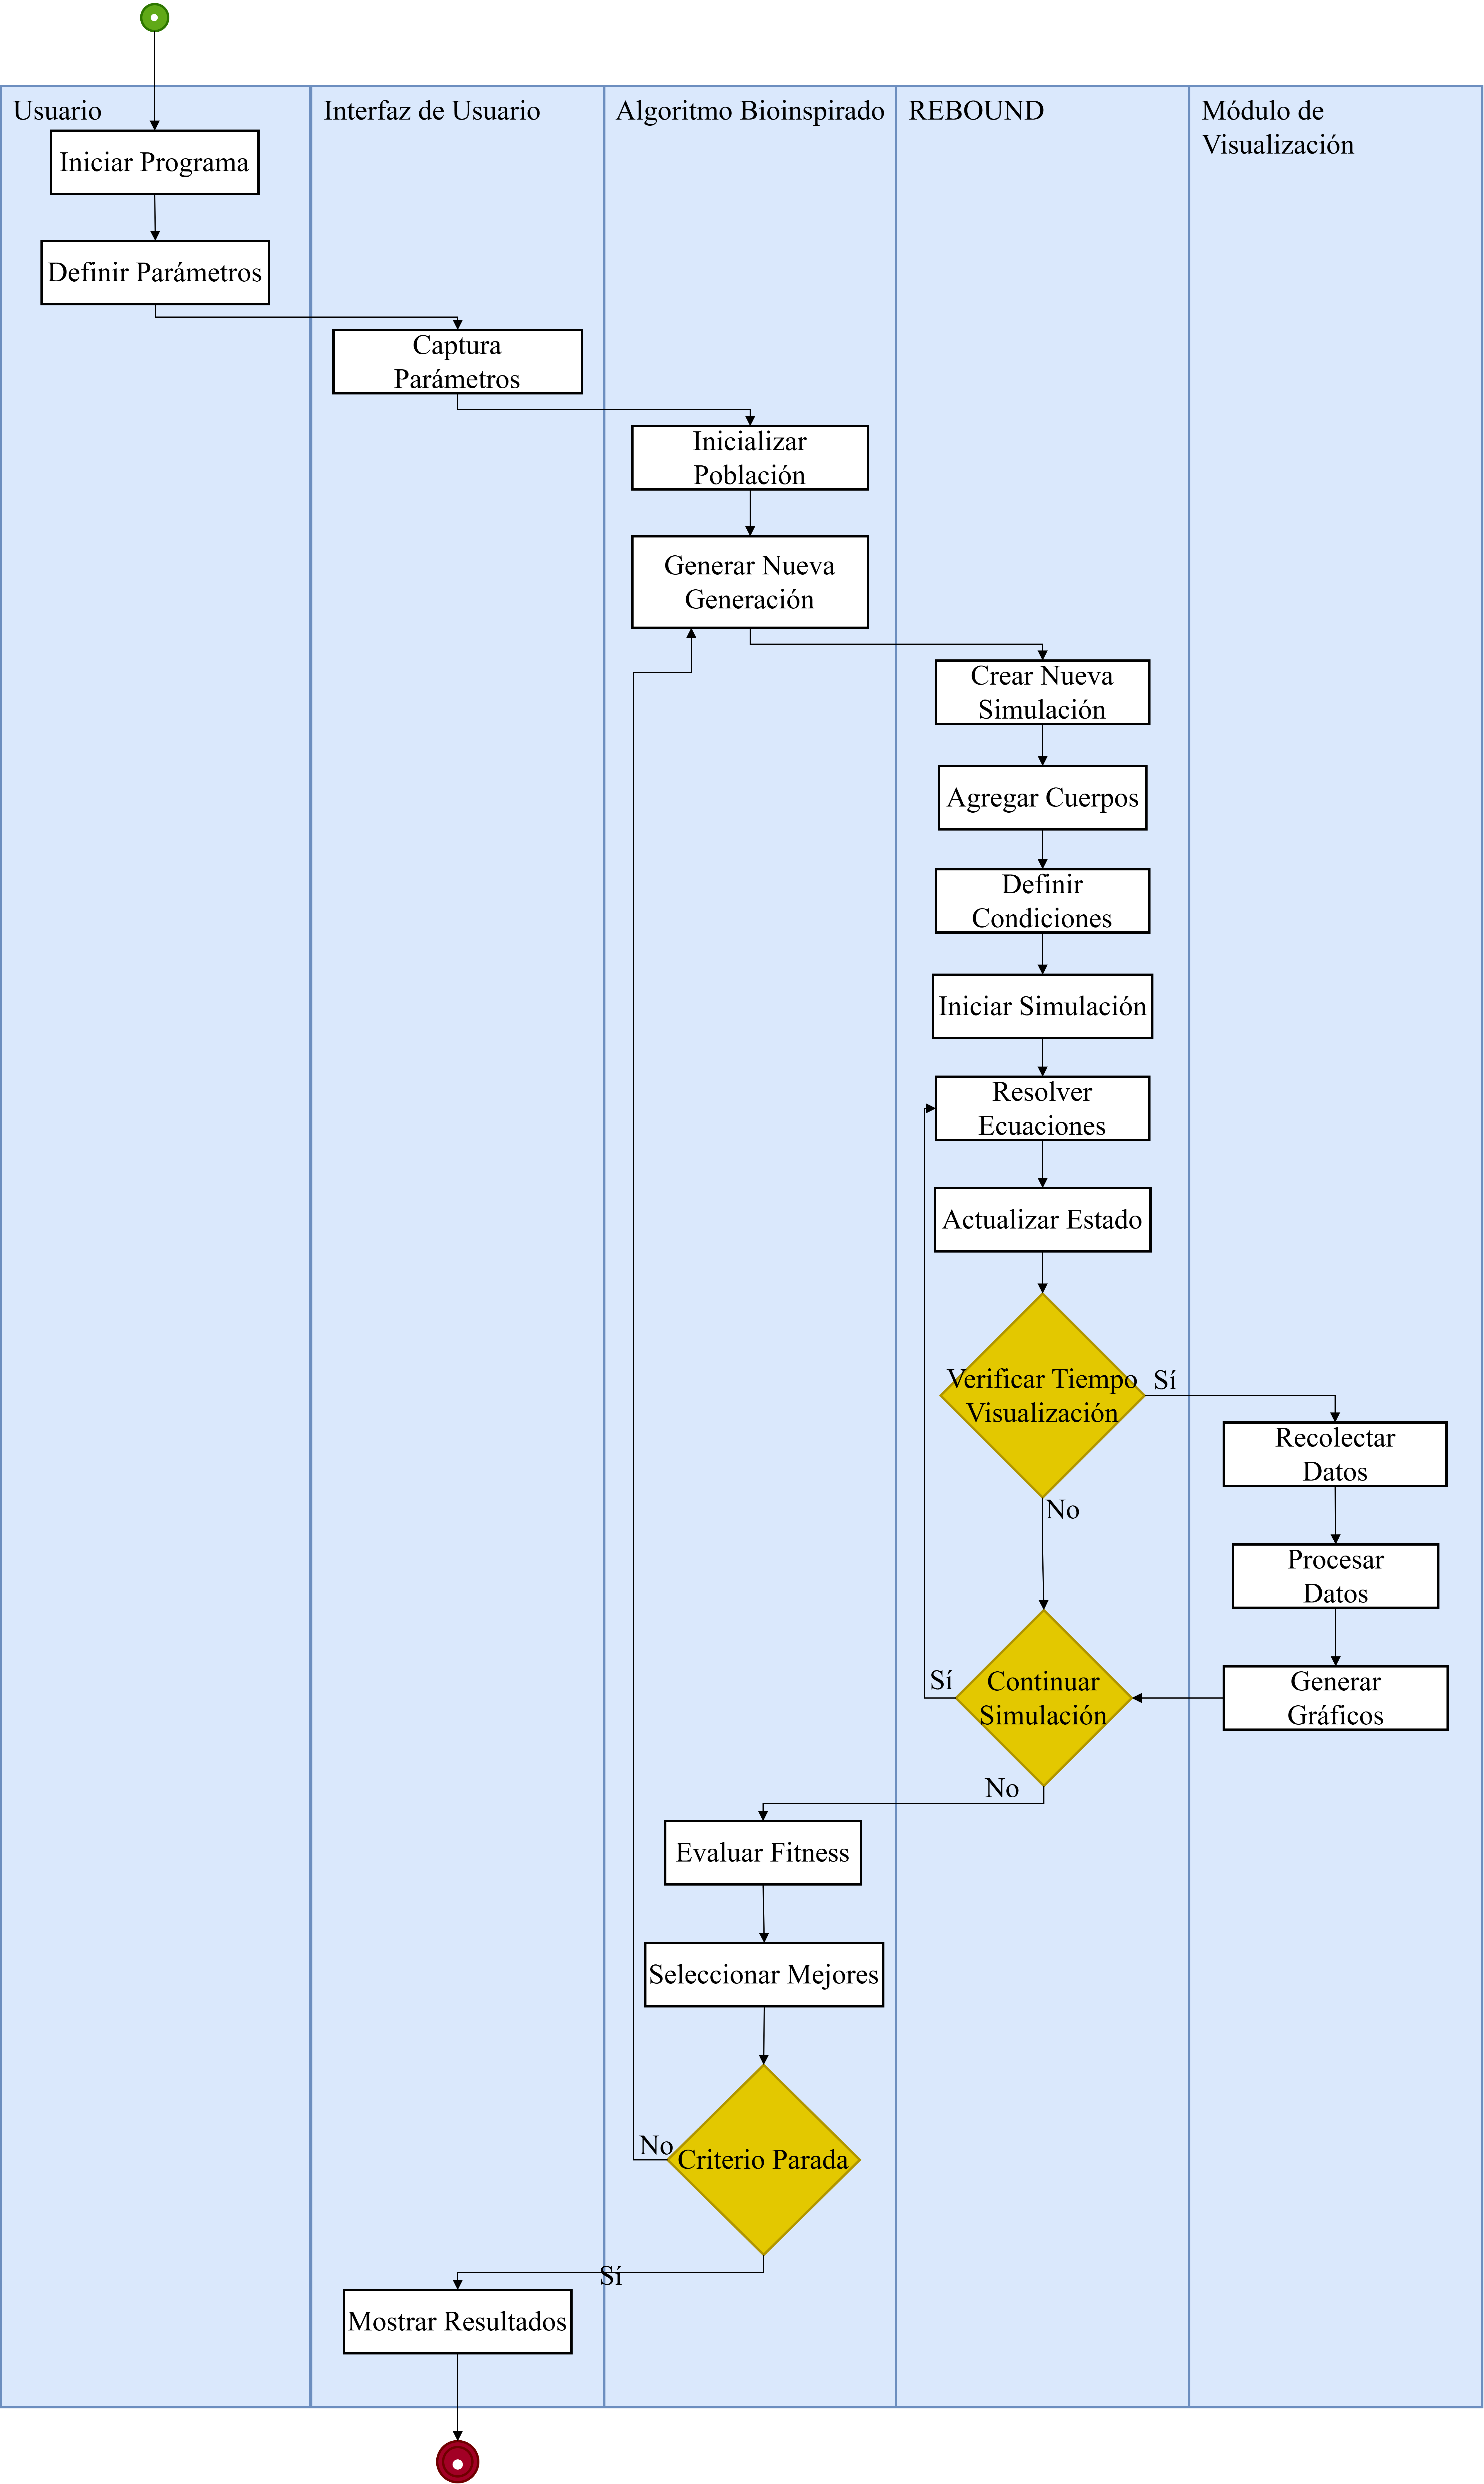
\includegraphics[width=\textwidth]{img/Analisis/DiagramaActividades2.png}
    \caption{Diagrama de Actividades UML del proceso de simulación y optimización.}%
    \label{fig:activity_diagram} % Etiqueta para referenciar la figura
\end{figure}

\subsection{Descripción del Diagrama de Actividades}

\subsubsection{Estructura del Diagrama: Carriles (Swimlanes)}

El diagrama se organiza en cinco carriles (swimlanes), cada uno representando un actor o componente lógico del sistema, delineando sus responsabilidades específicas:

\begin{enumerate}
    \item \textbf{Usuario:} Representa al actor humano que interactúa con el sistema. Es responsable de iniciar la ejecución y proporcionar la configuración inicial requerida.
    \item \textbf{Interfaz de Usuario (UI):} Componente software que media la interacción entre el \textit{Usuario} y el núcleo del sistema. Gestiona la captura de parámetros de entrada y la presentación de resultados.
    \item \textbf{Algoritmo Bioinspirado:} Componente central responsable de la optimización. Administra la población de soluciones candidatas (conjuntos de parámetros), aplica operadores evolutivos (generación, evaluación, selección) y determina la terminación del proceso según criterios definidos.
    \item \textbf{REBOUND:} Representa la biblioteca de simulación gravitacional. Ejecuta simulaciones de N-cuerpos (inicialmente, 2 cuerpos) basadas en los parámetros proporcionados por el \textit{Algoritmo Bioinspirado} para cada individuo evaluado. Cabe destacar que se instancia una nueva simulación para cada conjunto de parámetros a evaluar.
    \item \textbf{Módulo de Visualización:} Componente encargado de generar representaciones gráficas del estado del sistema en instantes de tiempo específicos, definidos por el \textit{Usuario}, para el monitoreo de la evolución dinámica.
\end{enumerate}

\subsubsection{Flujo Detallado de Actividades}

El proceso modelado en el diagrama sigue la secuencia lógica que se describe a continuación:

\begin{enumerate}
    \item \textbf{Inicialización y Configuración:}
        \begin{itemize}
            \item El \textit{Usuario} inicia la ejecución de la aplicación (\textbf{Iniciar Programa}).
            \item El \textit{Usuario} especifica los parámetros de configuración inicial, incluyendo rangos de búsqueda para la optimización, la función objetivo, criterios de parada, y los instantes discretos de tiempo para la visualización (\textbf{Definir Parámetros}).
            \item La \textit{Interfaz de Usuario} captura y valida esta información (\textbf{Captura Parámetros}).
        \end{itemize}

    \item \textbf{Ciclo Iterativo de Optimización y Simulación:}
        \begin{itemize}
            \item La \textit{UI} transmite los parámetros de configuración al \textit{Algoritmo Bioinspirado}, el cual inicializa su población de soluciones candidatas (\textbf{Inicializar Población}).
            \item \textbf{Inicio del Bucle de Optimización:} El algoritmo genera una nueva generación de conjuntos de parámetros candidatos aplicando sus operadores definidos (\textbf{Generar Nueva Generación}).
            \item \textbf{Ejecución de Simulaciones por Individuo:} Para cada conjunto de parámetros (individuo) en la generación actual:
                \begin{itemize}
                    \item Se instruye a \textit{REBOUND} para crear una nueva instancia de simulación (\textbf{Crear Nueva Simulación}).
                    \item Se añaden los cuerpos celestes al entorno de simulación con las propiedades especificadas por el conjunto de parámetros actual (\textbf{Agregar Cuerpos}).
                    \item Se configuran las condiciones restantes de la simulación, como el integrador numérico y el paso de tiempo (\textbf{Definir Condiciones}).
                    \item \textit{REBOUND} inicia la simulación (\textbf{Iniciar Simulación}).
                    \item \textbf{Bucle Interno de Simulación (REBOUND):}
                        \begin{itemize}
                            \item \textit{REBOUND} resuelve las ecuaciones de movimiento para avanzar un paso de tiempo (\textbf{Resolver Ecuaciones}).
                            \item Actualiza el estado del sistema (posiciones, velocidades) (\textbf{Actualizar Estado}).
                            \item Verifica si el tiempo de simulación actual ($t_{\text{sim}}$) corresponde a uno de los instantes de visualización solicitados ($t_{\text{vis}}$) (\textbf{Verificar Tiempo Visualización}).
                            \item Si $t_{\text{sim}} = t_{\text{vis}}$ (Condición Verdadera): Se activa el \textit{Módulo de Visualización}, que recolecta los datos relevantes del estado actual (\textbf{Recolectar Datos}), los procesa (\textbf{Procesar Datos}) y genera la salida gráfica correspondiente (\textbf{Generar Gráficos}). La simulación continúa.
                            \item Si $t_{\text{sim}} \neq t_{\text{vis}}$ (Condición Falsa): La simulación continúa directamente al siguiente paso.
                            \item \textit{REBOUND} verifica si se ha alcanzado la condición de término de la simulación (p.\ ej., tiempo final $T_{\text{max}}$) (\textbf{Continuar Simulación}). Si no se ha alcanzado (Condición Falsa), retorna a \textbf{Resolver Ecuaciones}. Si se ha alcanzado (Condición Verdadera: \textbf{Simulación Terminada}), la ejecución para este individuo finaliza.
                        \end{itemize}
                \end{itemize}
            \item \textbf{Evaluación:} Tras la finalización de la simulación para un individuo, el \textit{Algoritmo Bioinspirado} utiliza los resultados (p.\ ej., una métrica derivada del estado final o la trayectoria) para calcular su valor de aptitud (fitness) (\textbf{Evaluar Fitness}). Este paso se repite para todos los individuos de la generación.
            \item \textbf{Selección y Criterio de Parada:} El \textit{Algoritmo Bioinspirado} aplica sus mecanismos de selección basados en la aptitud calculada (\textbf{Seleccionar Mejores}) y verifica si se cumple el criterio global de parada (p.\ ej., número máximo de generaciones, convergencia de la aptitud) (\textbf{Criterio Parada}).
                \begin{itemize}
                    \item Si el criterio no se cumple (Condición Falsa): Se procede a generar la siguiente generación (\textbf{Generar Nueva Generación}), continuando el ciclo de optimización.
                    \item Si el criterio se cumple (Condición Verdadera): El ciclo de optimización concluye.
                \end{itemize}
        \end{itemize}

    \item \textbf{Finalización:}
        \begin{itemize}
            \item El \textit{Algoritmo Bioinspirado} transfiere la mejor solución encontrada (conjunto de parámetros óptimos y su aptitud asociada) a la \textit{Interfaz de Usuario}.
            \item La \textit{Interfaz de Usuario} presenta los resultados finales al \textit{Usuario} (\textbf{Mostrar Resultados}).
            \item El proceso finaliza (nodo final de actividad). % O referenciar el símbolo específico si se usa en el diagrama
        \end{itemize}
\end{enumerate}

\subsection{Aspectos Clave del Diseño Reflejados en el Diagrama}

El diagrama de actividades pone de manifiesto varios aspectos fundamentales del diseño del sistema:

\begin{itemize}
    \item \textbf{Modularidad y Separación de Responsabilidades:} La estructura en carriles delimita claramente las funciones del componente de optimización (\textit{Algoritmo Bioinspirado}) y del componente de simulación física (\textit{REBOUND}), promoviendo un diseño modular.
    \item \textbf{Naturaleza Iterativa del Proceso:} El bucle principal que engloba \textbf{Generar Nueva Generación}, la ejecución de simulaciones en \textit{REBOUND}, \textbf{Evaluar Fitness} y \textbf{Criterio Parada} representa visualmente el núcleo iterativo característico de los algoritmos evolutivos y otros métodos de optimización bioinspirados.
    \item \textbf{Simulación como Evaluación de Aptitud:} Desde la perspectiva del optimizador, el módulo \textit{REBOUND} actúa como una función objetivo (o parte de ella), evaluando la calidad (aptitud) de un conjunto de parámetros candidato mediante la ejecución de una simulación física.
    \item \textbf{Instanciación Independiente de Simulaciones:} El flujo muestra que cada evaluación de un individuo dentro del ciclo de optimización requiere la creación y ejecución de una nueva instancia de simulación en \textit{REBOUND}, configurada con los parámetros específicos de dicho individuo.
    \item \textbf{Control Discreto de la Visualización:} La generación de visualizaciones está integrada en el bucle de simulación de \textit{REBOUND} pero se activa únicamente en puntos temporales discretos especificados por el \textit{Usuario}, evitando una sobrecarga continua.
\end{itemize}

    \begin{figure}[H]
    \centering
    \includegraphics[width=\textwidth]{img/Analisis/DiagramaProcesos/DiagramaProceso01_Captura Parámetros.png}
    \caption{Diagrama de Proceso Interno 01: Captura de Paráametros}%
    \label{fig:process_diagram01}
\end{figure}

\begin{figure}[H]
    \centering
    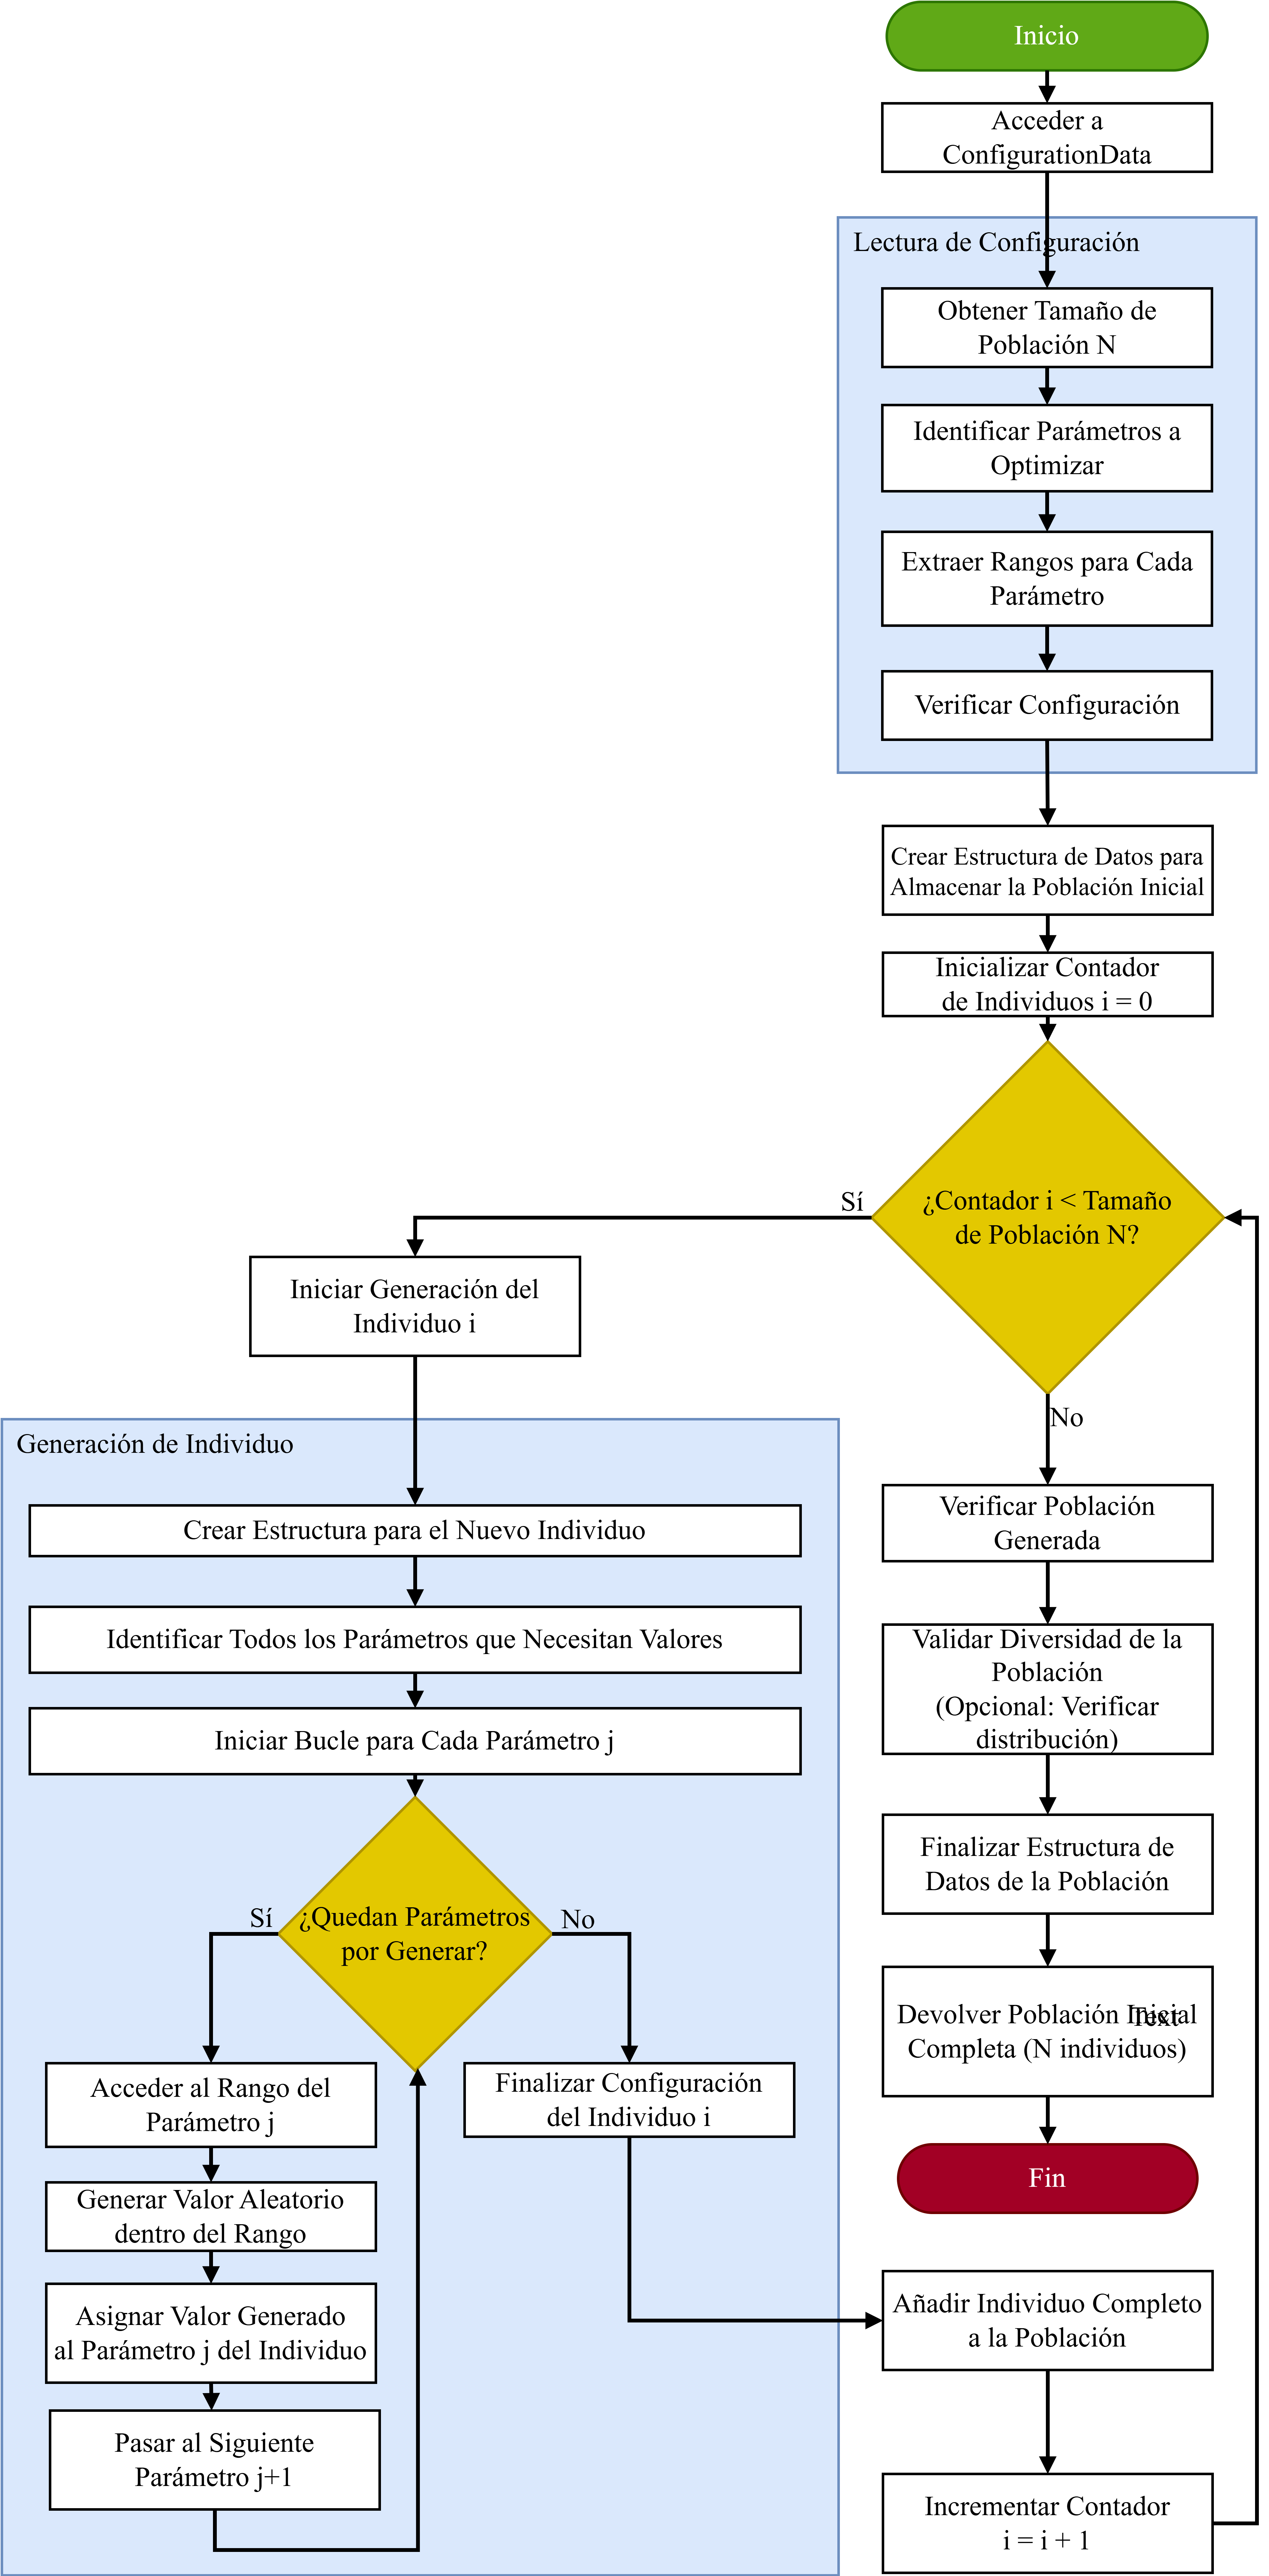
\includegraphics[width=\textwidth]{img/Analisis/DiagramaProcesos/DiagramaProceso02_InicializarPoblacion.png}
    \caption{Diagrama de Proceso Interno 02: Inicializar Población}%
    \label{fig:process_diagram02}
\end{figure}

\begin{figure}[H]
    \centering
    \includegraphics[width=\textwidth]{img/Analisis/DiagramaProcesos/DiagramaProceso03_GenerarNuevaGeneración.png}
    \caption{Diagrama de Proceso Interno 03: Generar Nueva Generación}%
    \label{fig:process_diagram03}
\end{figure}

\begin{figure}[H]
    \centering
    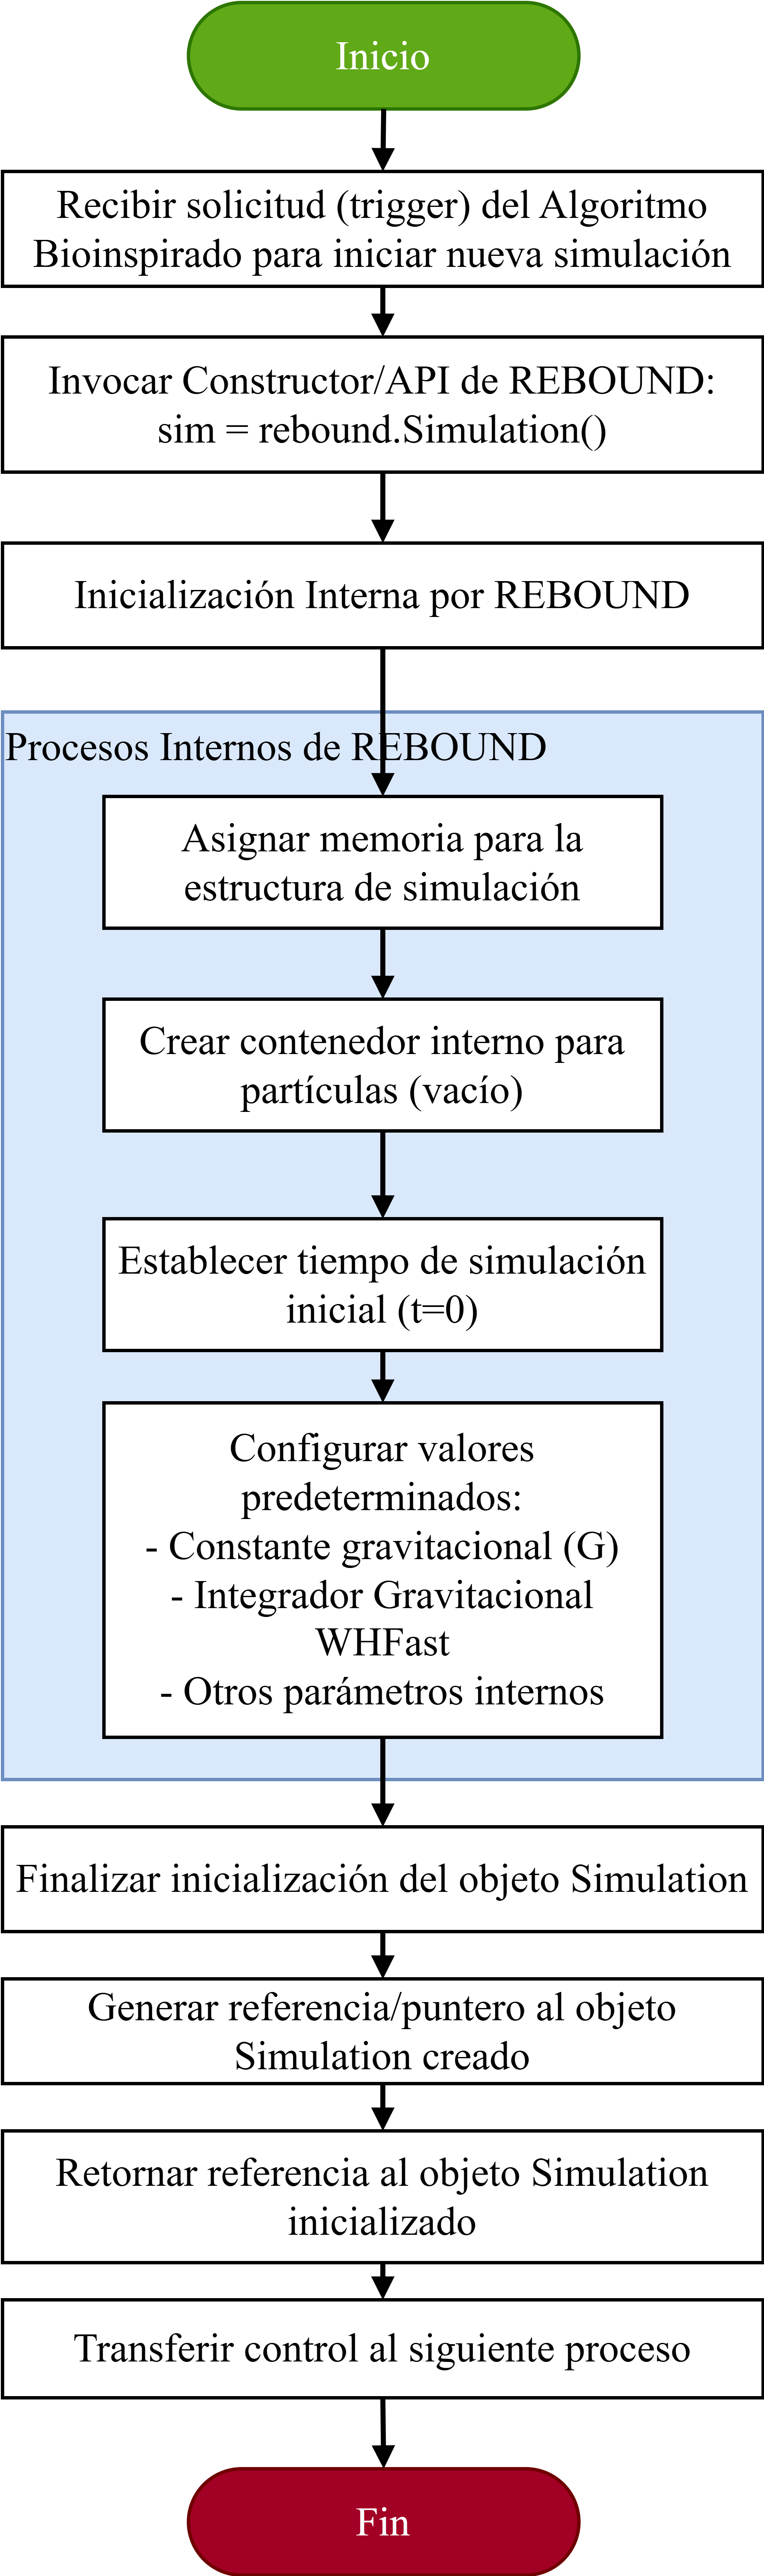
\includegraphics[width=\textwidth]{img/Analisis/DiagramaProcesos/DiagramaProceso04_CrearSimulacion.png}
    \caption{Diagrama de Proceso Interno 04: Crear Simulación}%
    \label{fig:process_diagram04}
\end{figure}

\begin{figure}[H]
    \centering
    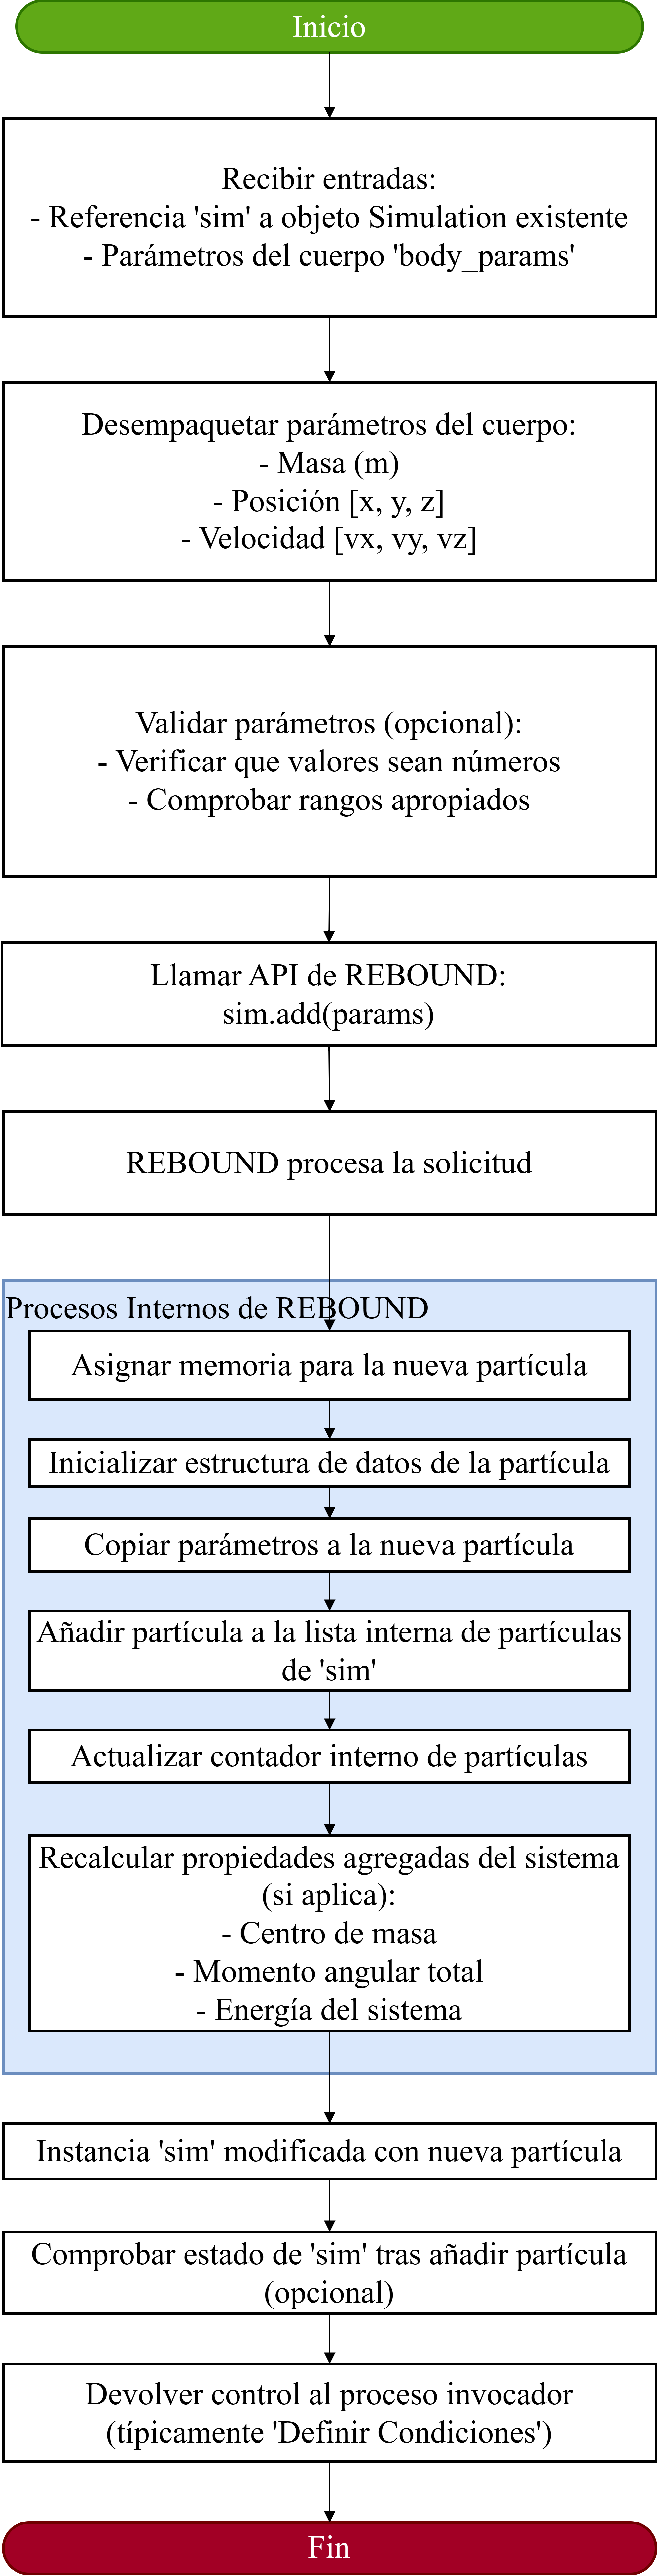
\includegraphics[width=\textwidth]{img/Analisis/DiagramaProcesos/DiagramaProceso05AgregarCuerpos.png}
    \caption{Diagrama de Proceso Interno 05: Agregar Cuerpos}%
    \label{fig:process_diagram05}
\end{figure}

\begin{figure}[H]
    \centering
    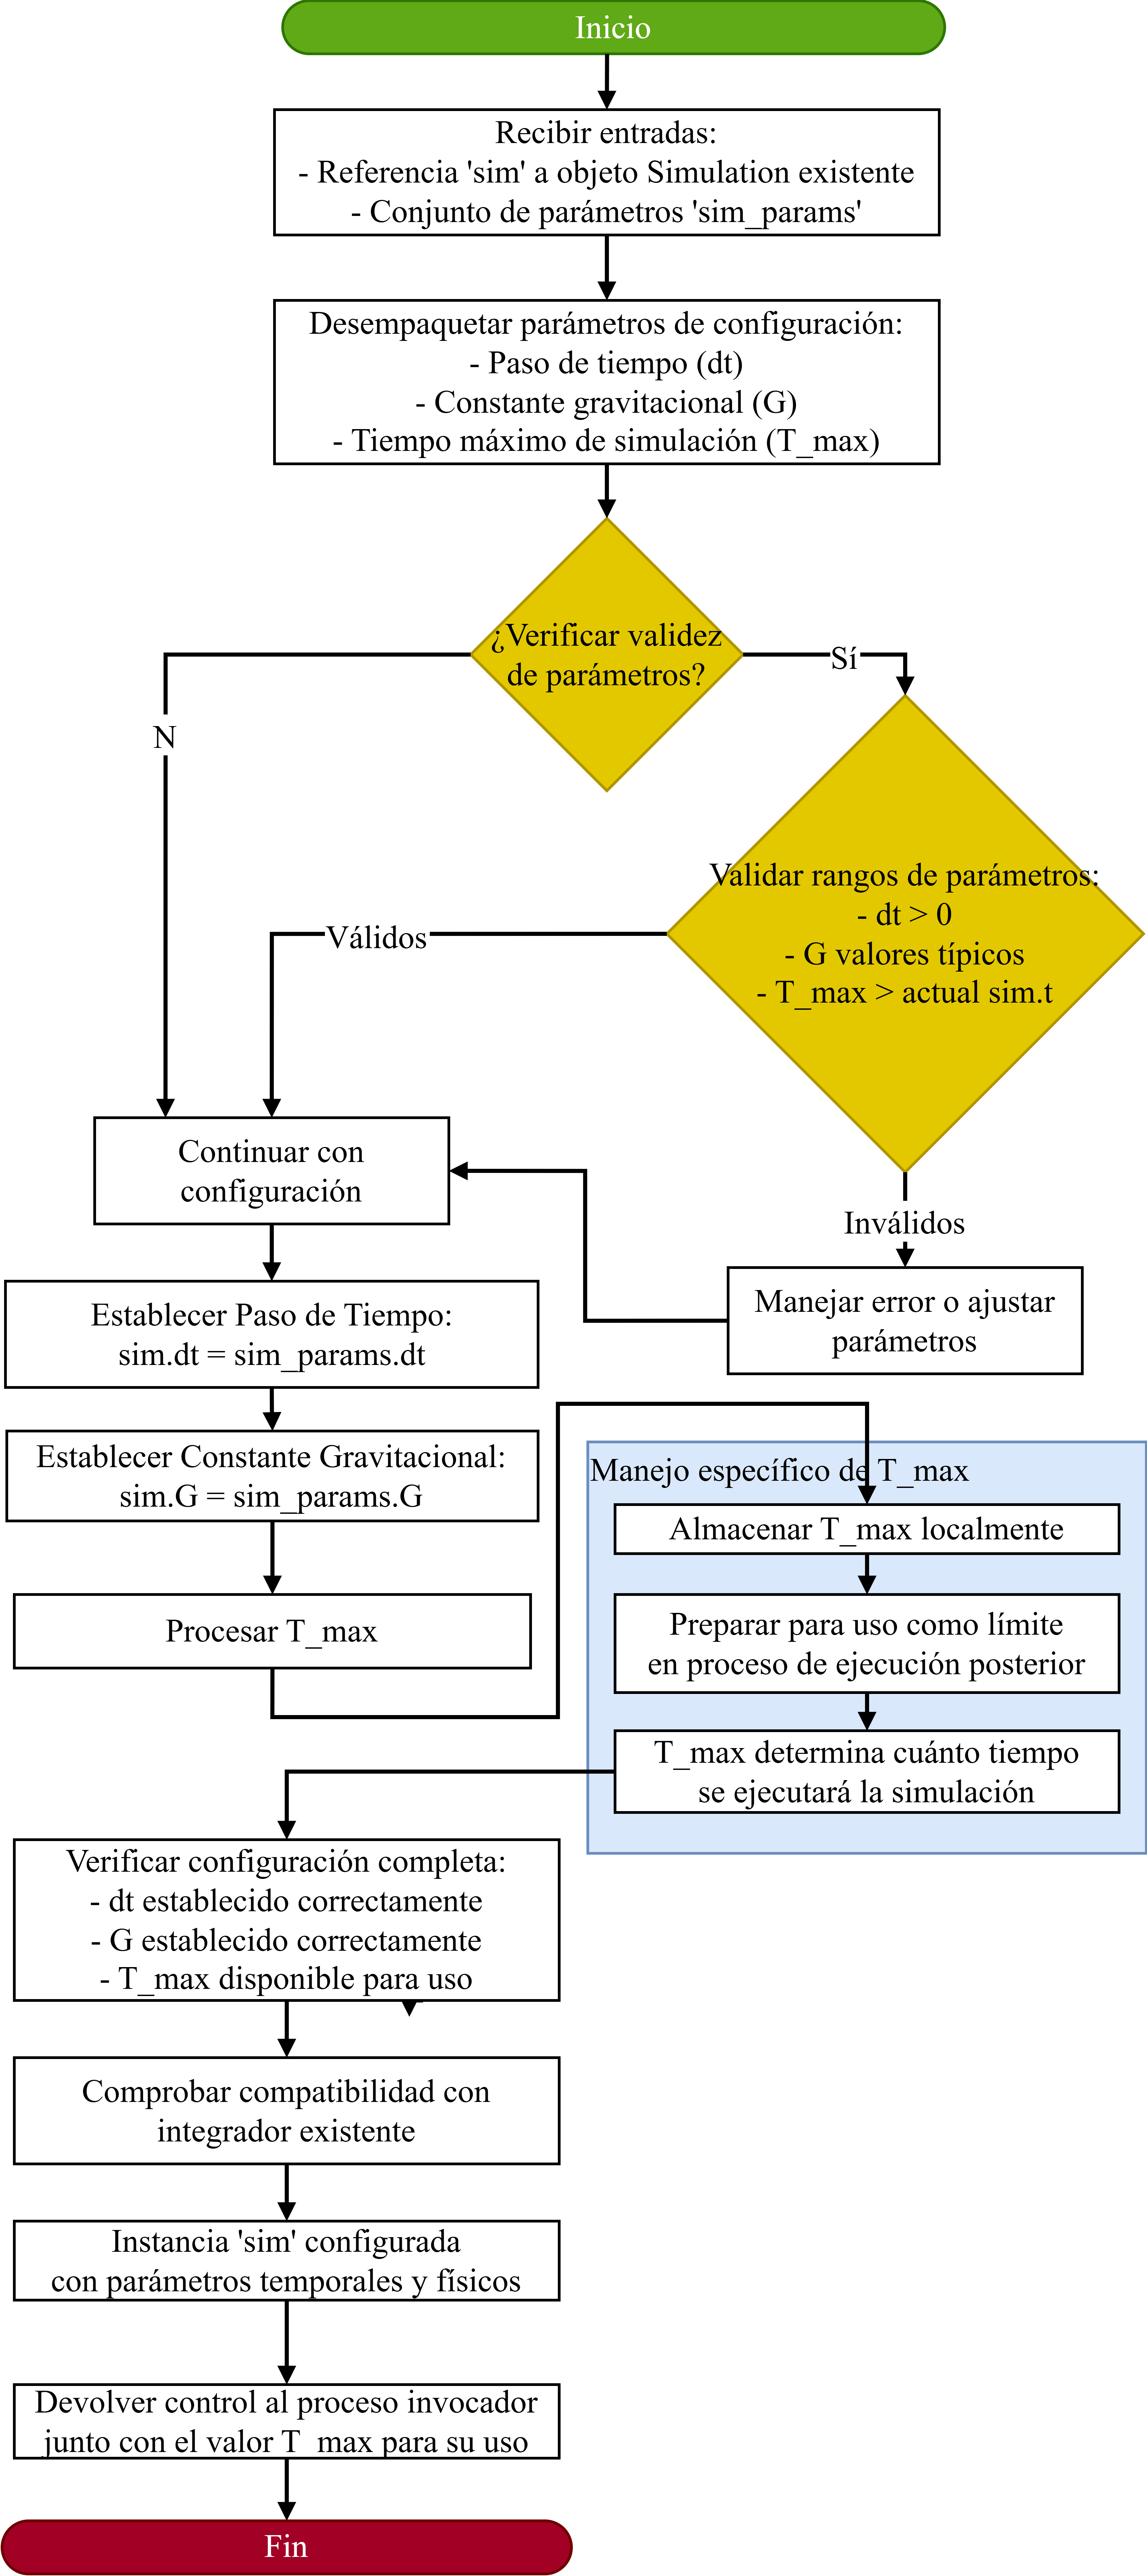
\includegraphics[width=\textwidth]{img/Analisis/DiagramaProcesos/DiagramaProceso06_DefinirCondiciones.png}
    \caption{Diagrama de Proceso Interno 06: Definir Condiciones}%
    \label{fig:process_diagram06}
\end{figure}

\begin{figure}[H]
    \centering
    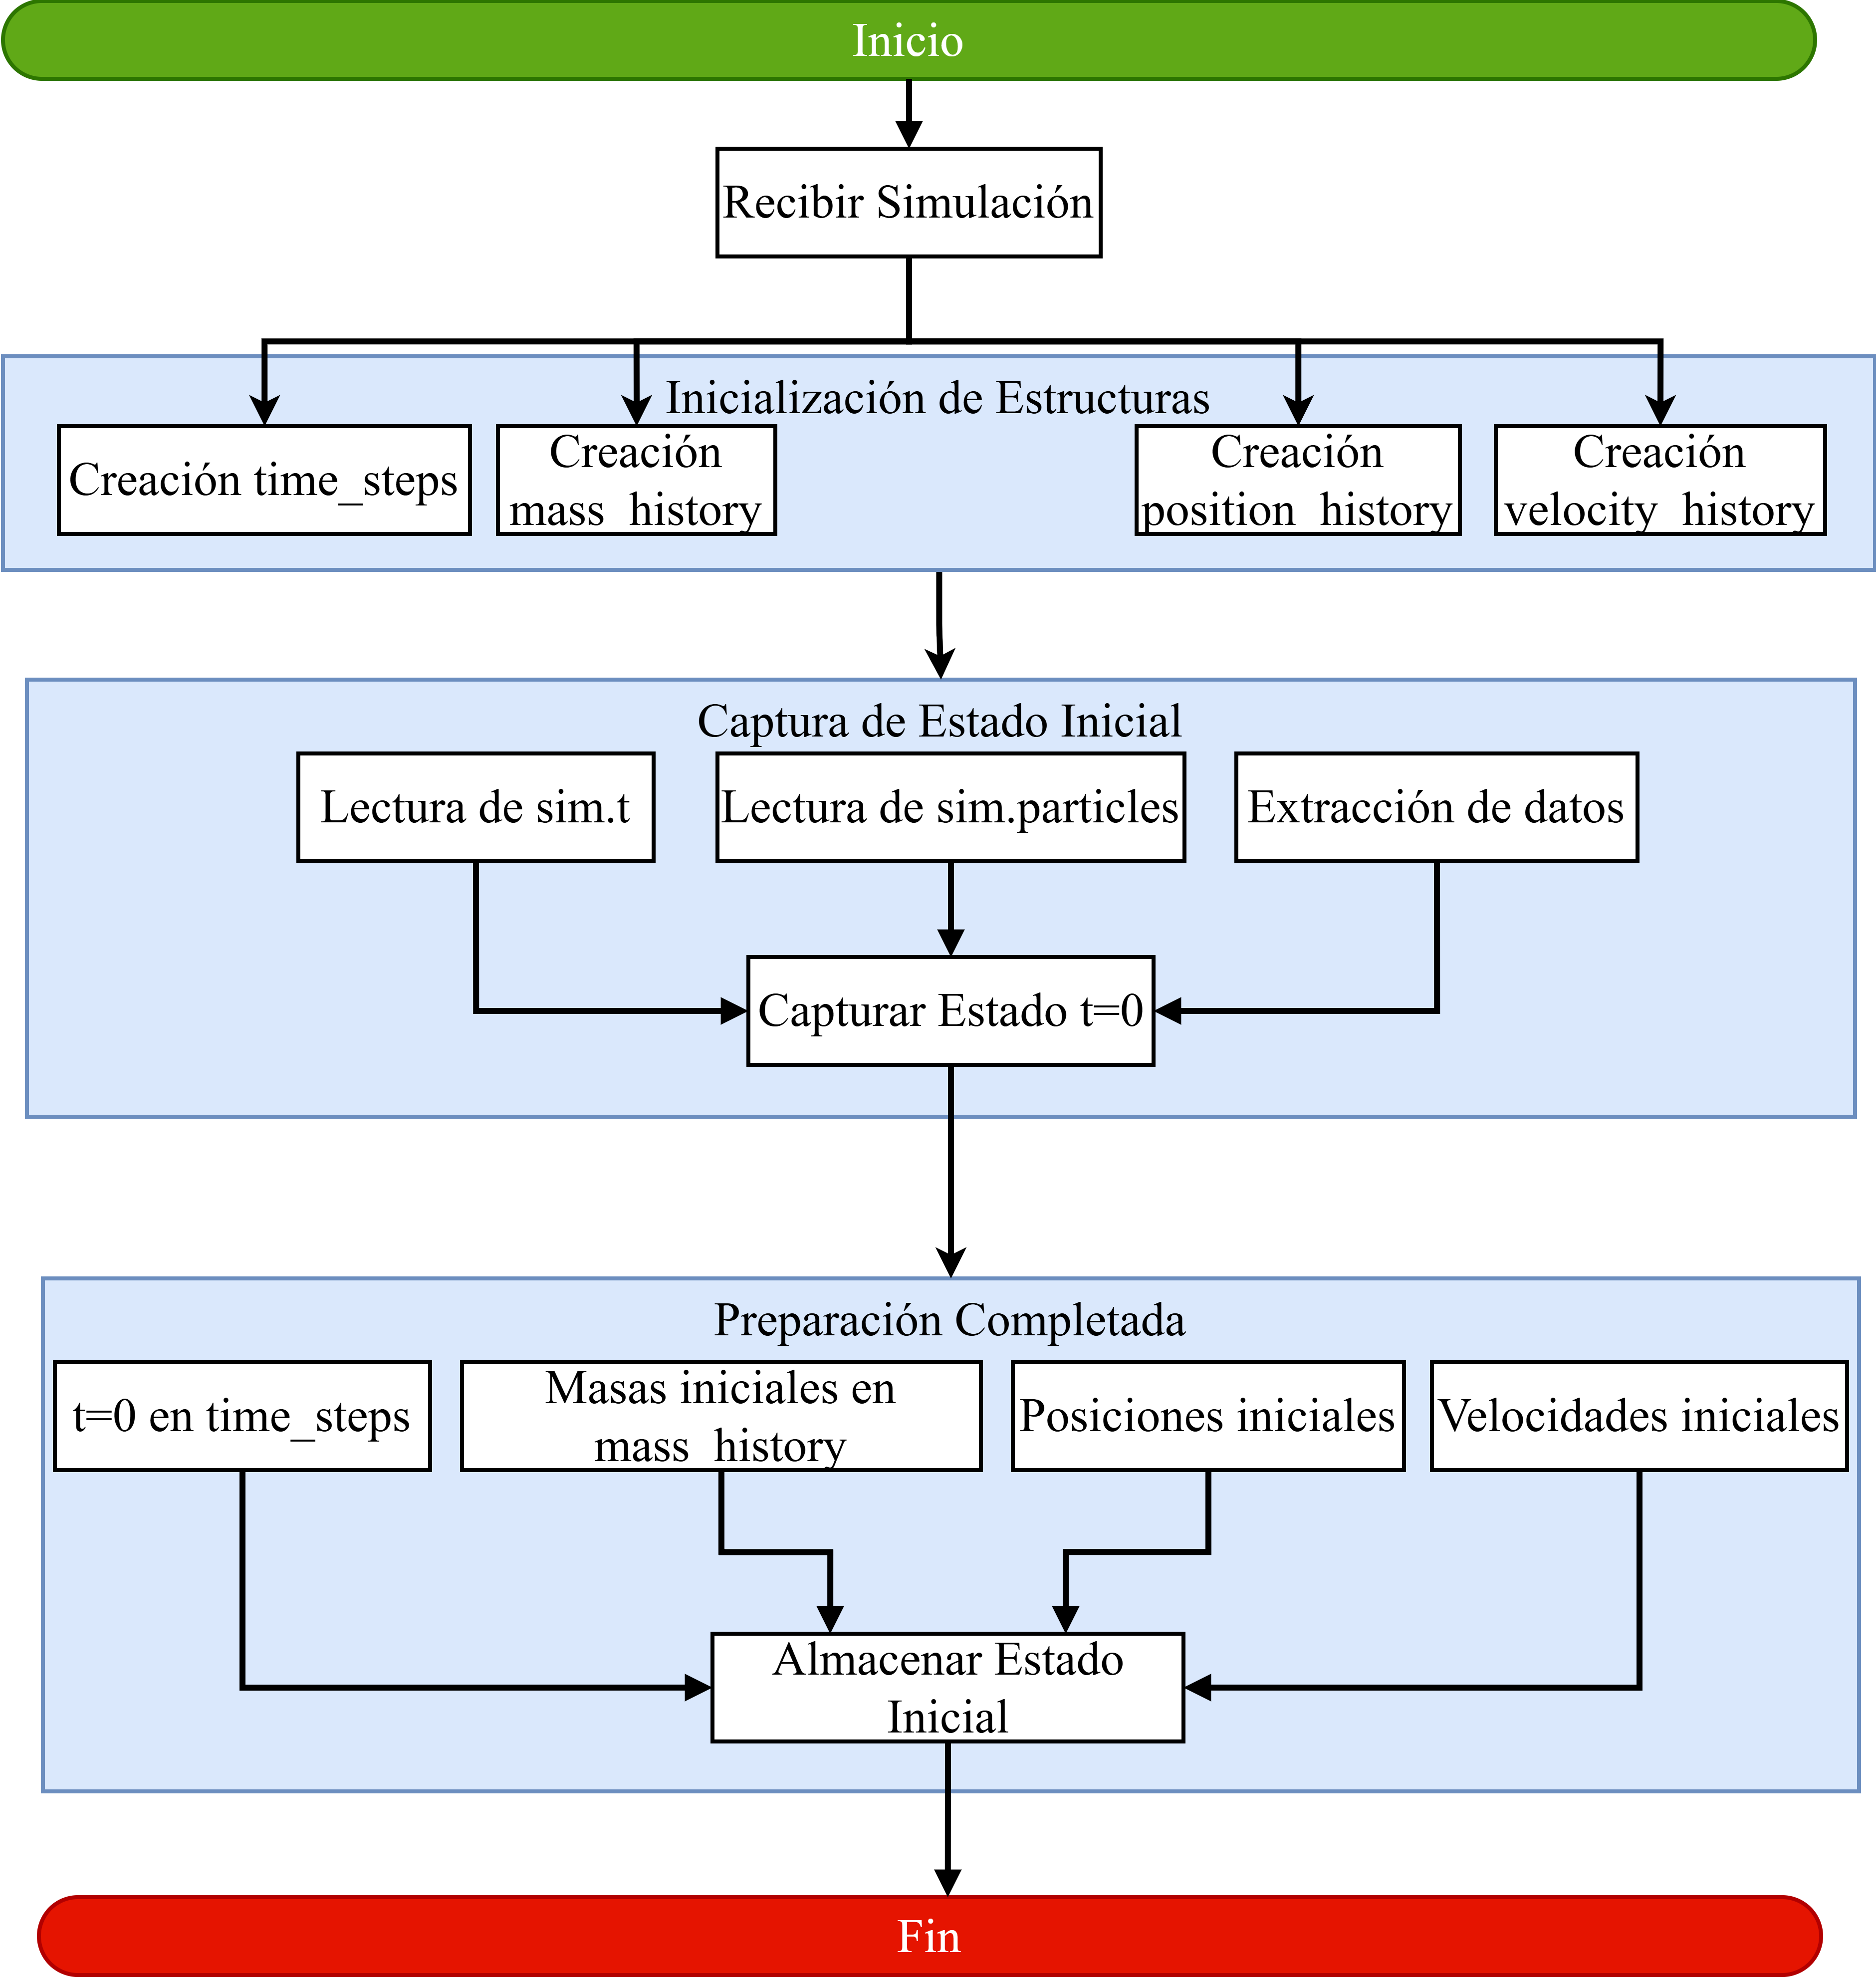
\includegraphics[width=\textwidth]{img/Analisis/DiagramaProcesos/DiagramaProceso07_IniciarSimulacion.png}
    \caption{Diagrama de Proceso Interno 07: Iniciar Simulación}%
    \label{fig:process_diagram07}
\end{figure}

\begin{figure}[H]
    \centering
    \includegraphics[width=\textwidth]{img/Analisis/DiagramaProcesos/DiagramaProceso08_ResolverEcuaciones.png}
    \caption{Diagrama de Proceso Interno 08: Resolver Ecuaciones}%
    \label{fig:process_diagram08}
\end{figure}

\begin{figure}[H]
    \centering
    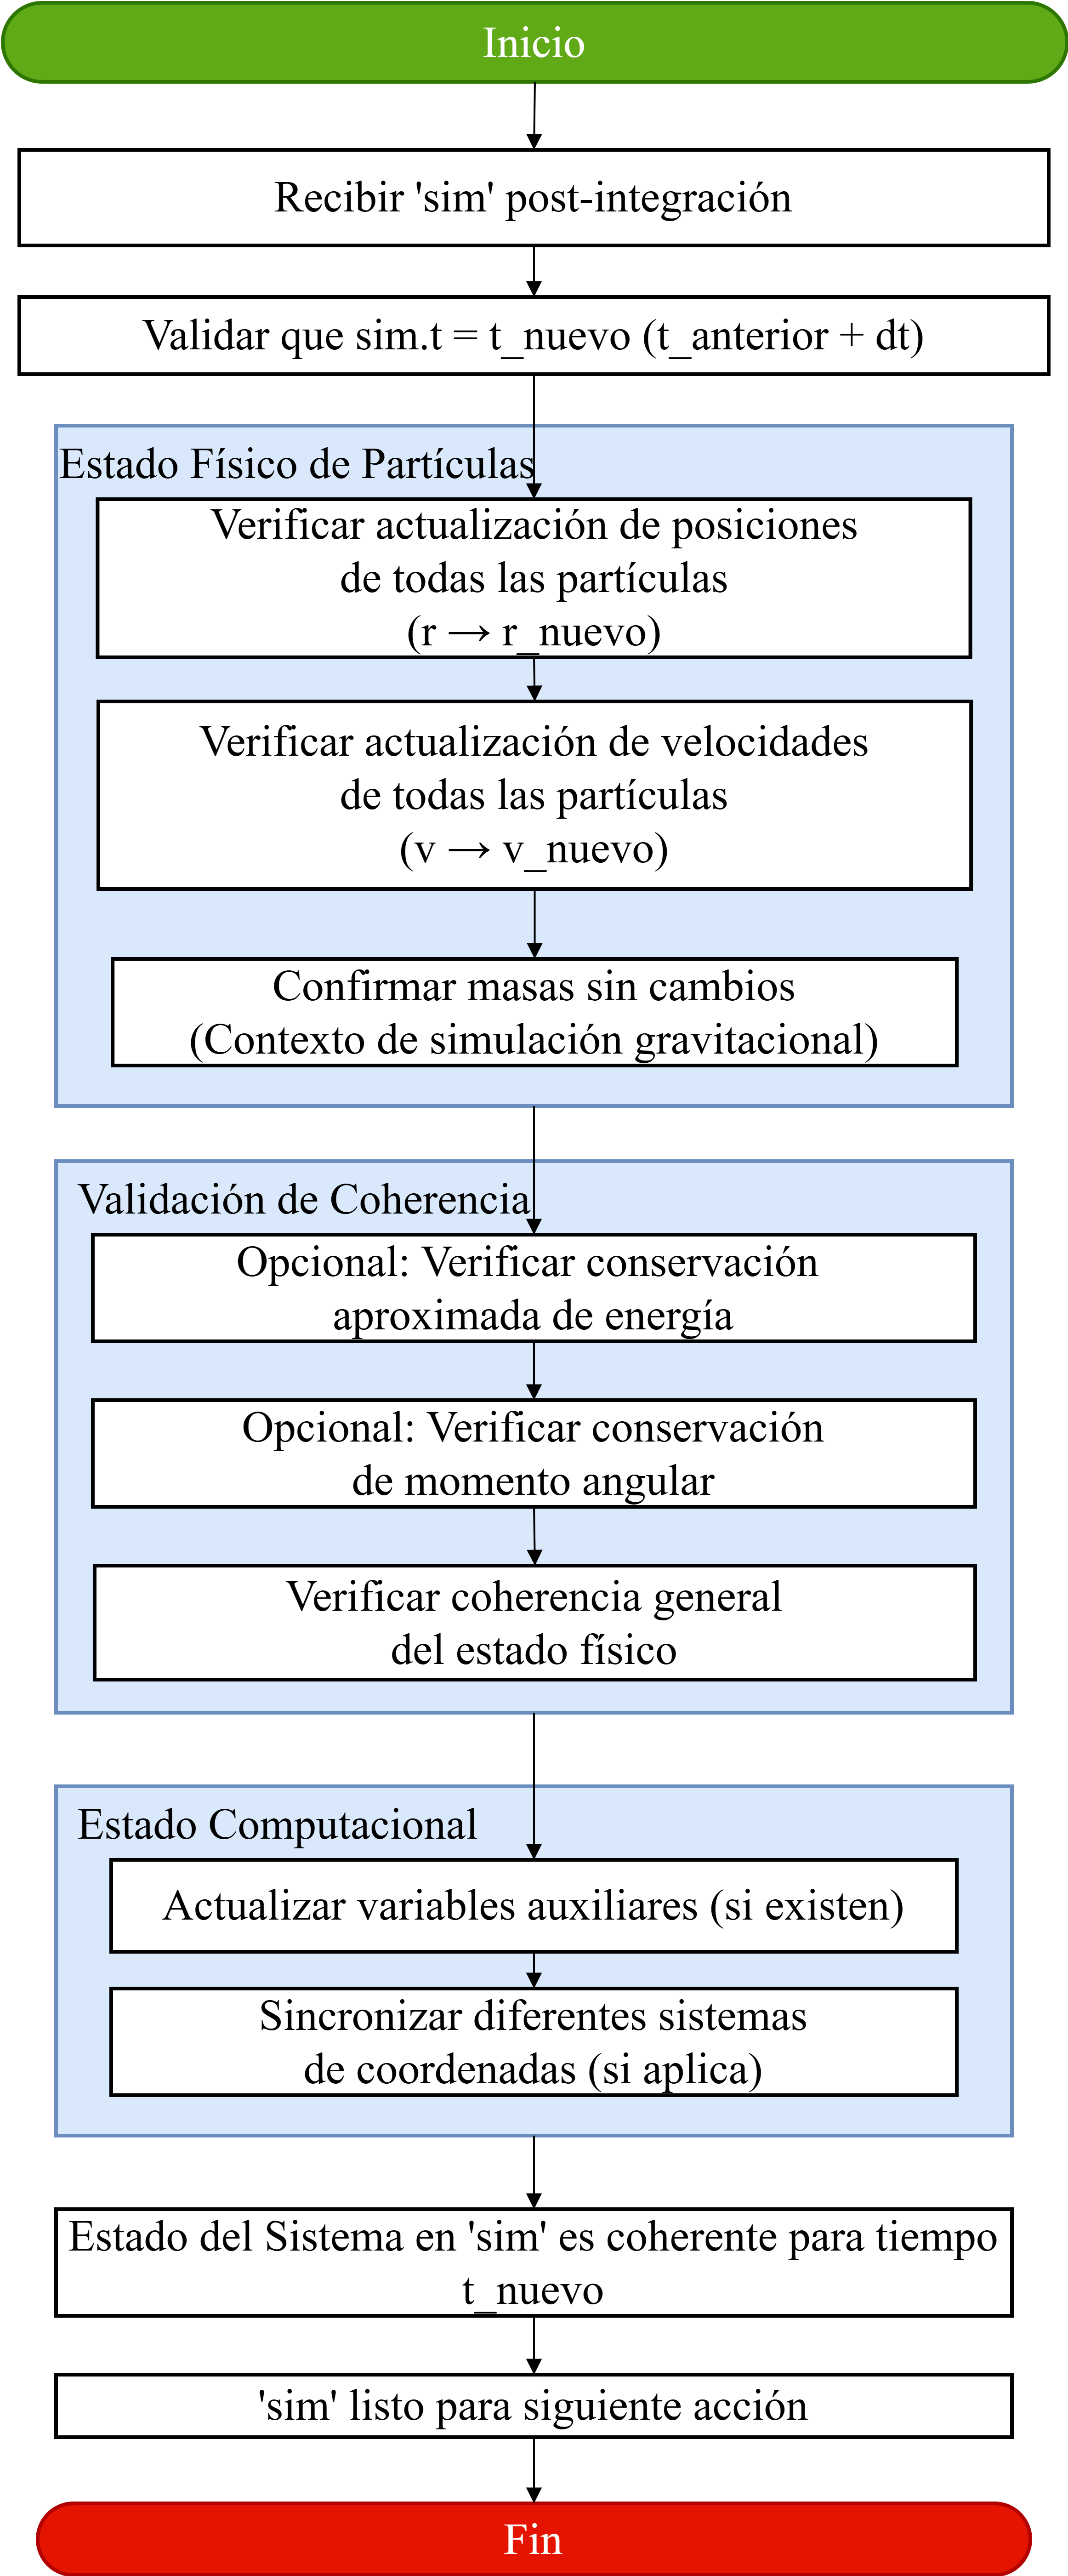
\includegraphics[width=\textwidth]{img/Analisis/DiagramaProcesos/DiagramaProceso09_ActualizarEstado.png}
    \caption{Diagrama de Proceso Interno 09: Actualizar Estado}%
    \label{fig:process_diagram09}
\end{figure}

\begin{figure}[H]
    \centering
    \includegraphics[width=\textwidth]{img/Analisis/DiagramaProcesos/DiagramaProceso10_RecolectarDatos.png}
    \caption{Diagrama de Proceso Interno 10: Recolectar Datos}%
    \label{fig:process_diagram10}
\end{figure}

\begin{figure}[H]
    \centering
    \includegraphics[width=\textwidth]{img/Analisis/DiagramaProcesos/DiagramaProceso011_ProcesarDatos.png}
    \caption{Diagrama de Proceso Interno 11: Procesa Datos}%
    \label{fig:process_diagram11}
\end{figure}

\begin{figure}[H]
    \centering
    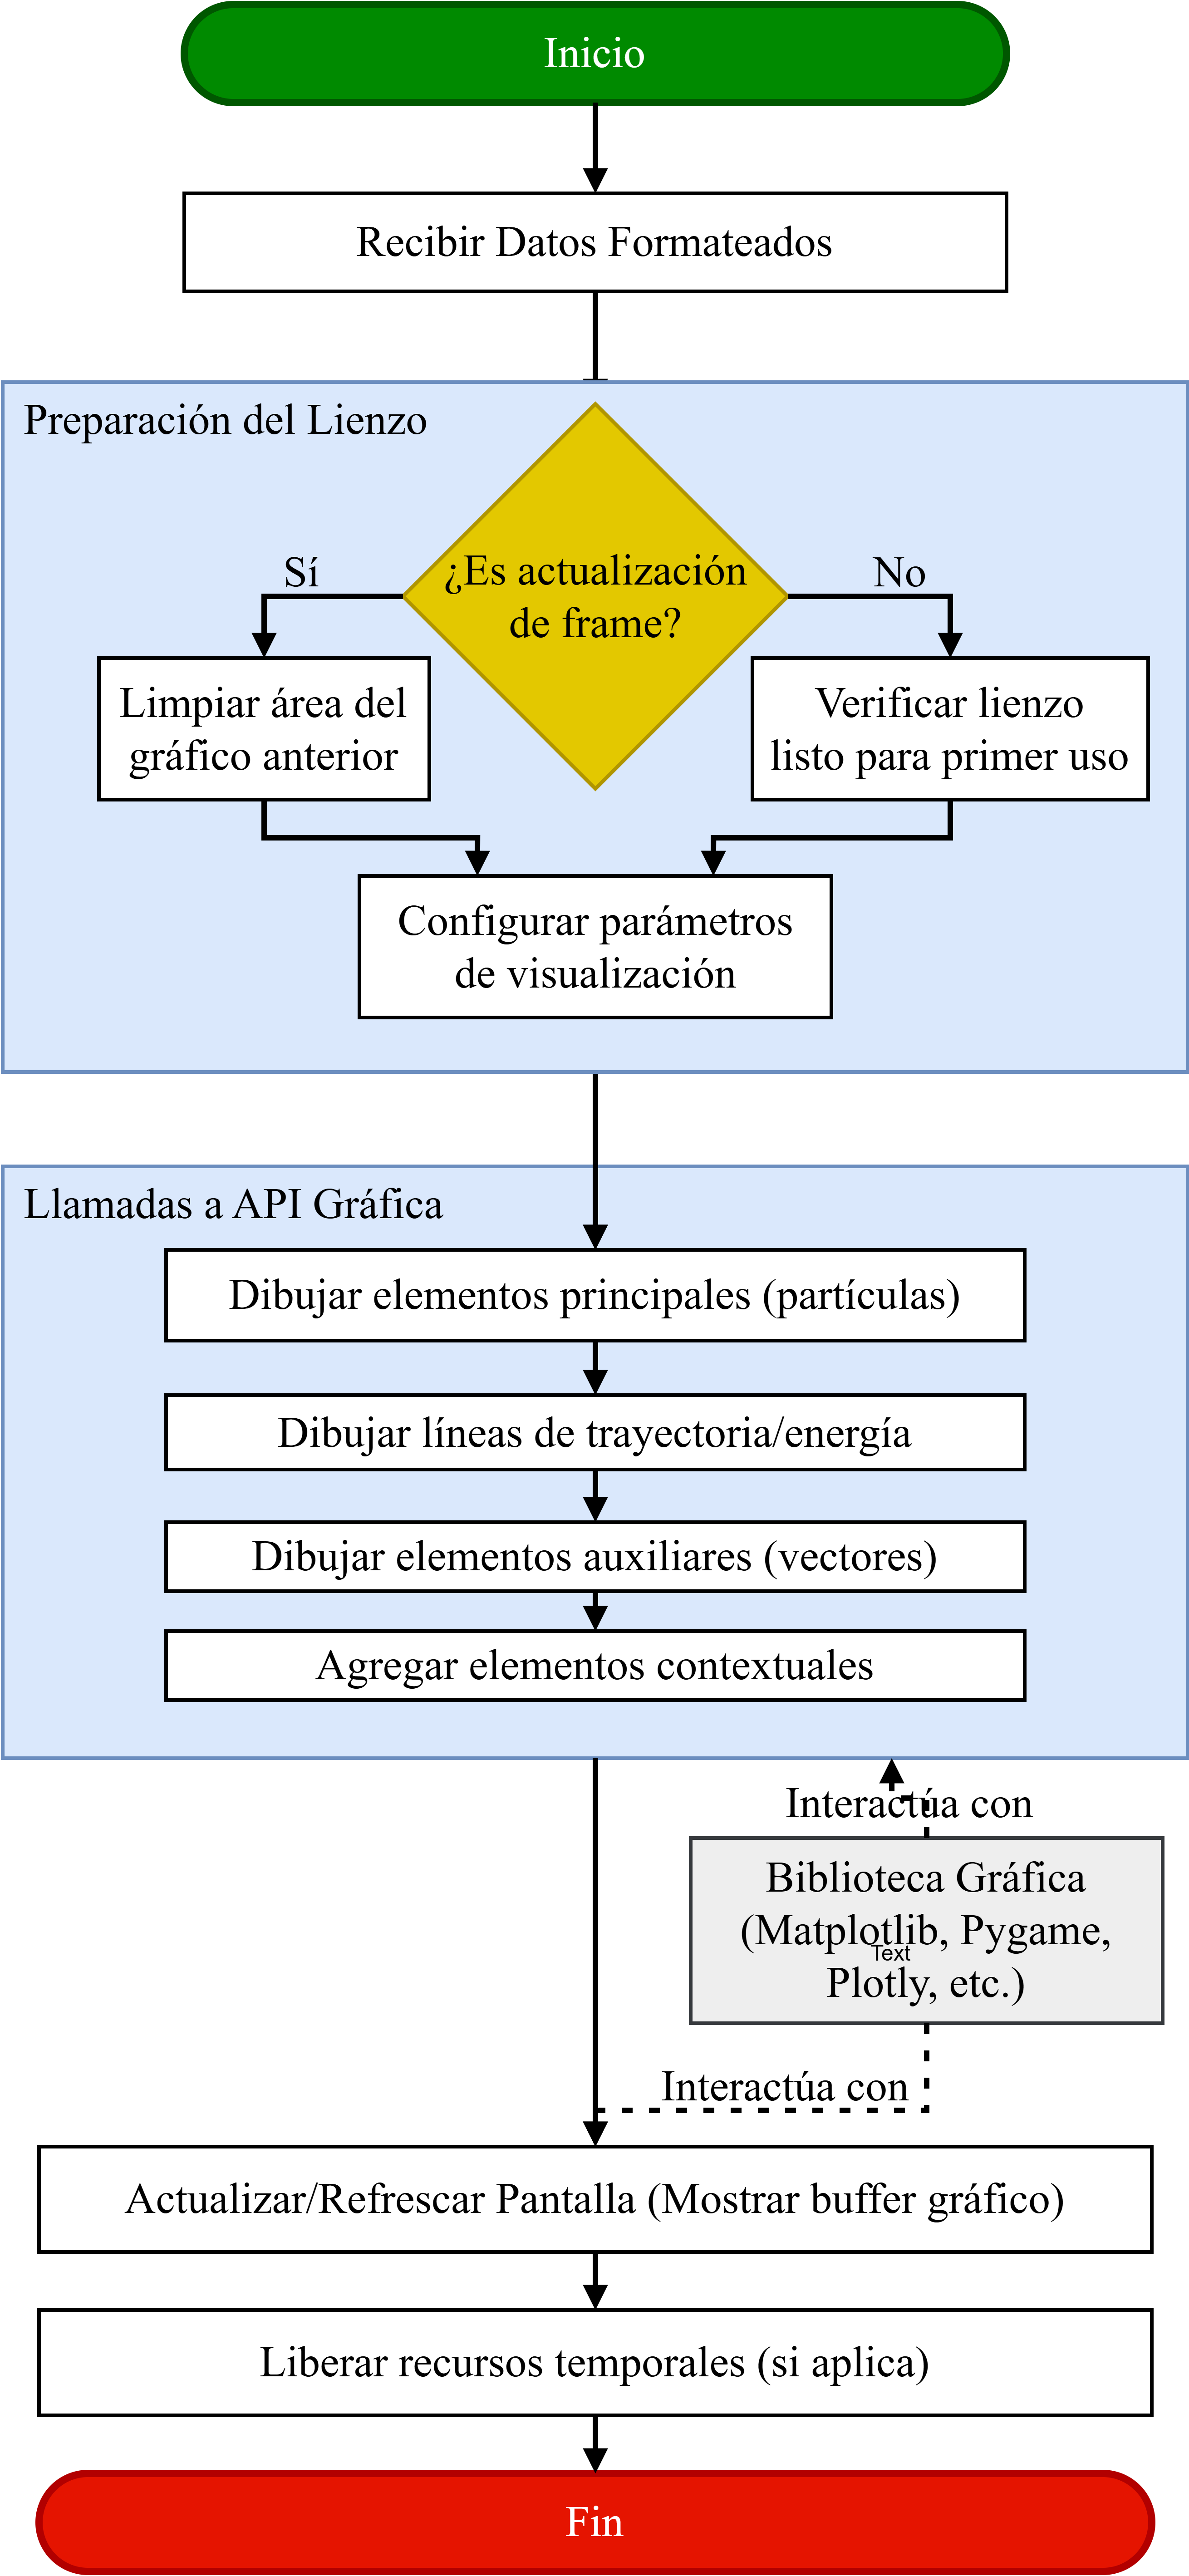
\includegraphics[width=\textwidth]{img/Analisis/DiagramaProcesos/DiagramaProceso12_GenerarGrafico.png}
    \caption{Diagrama de Proceso Interno 12: Generar Gráfico}%
    \label{fig:process_diagram12}
\end{figure}

\begin{figure}[H]
    \centering
    \includegraphics[width=\textwidth]{img/Analisis/DiagramaProcesos/DiagramaProceso13_CalcularFitness.png}
    \caption{Diagrama de Proceso Interno 13: Calcular Fitness}%
    \label{fig:process_diagram13}
\end{figure}

\begin{figure}[H]
    \centering
    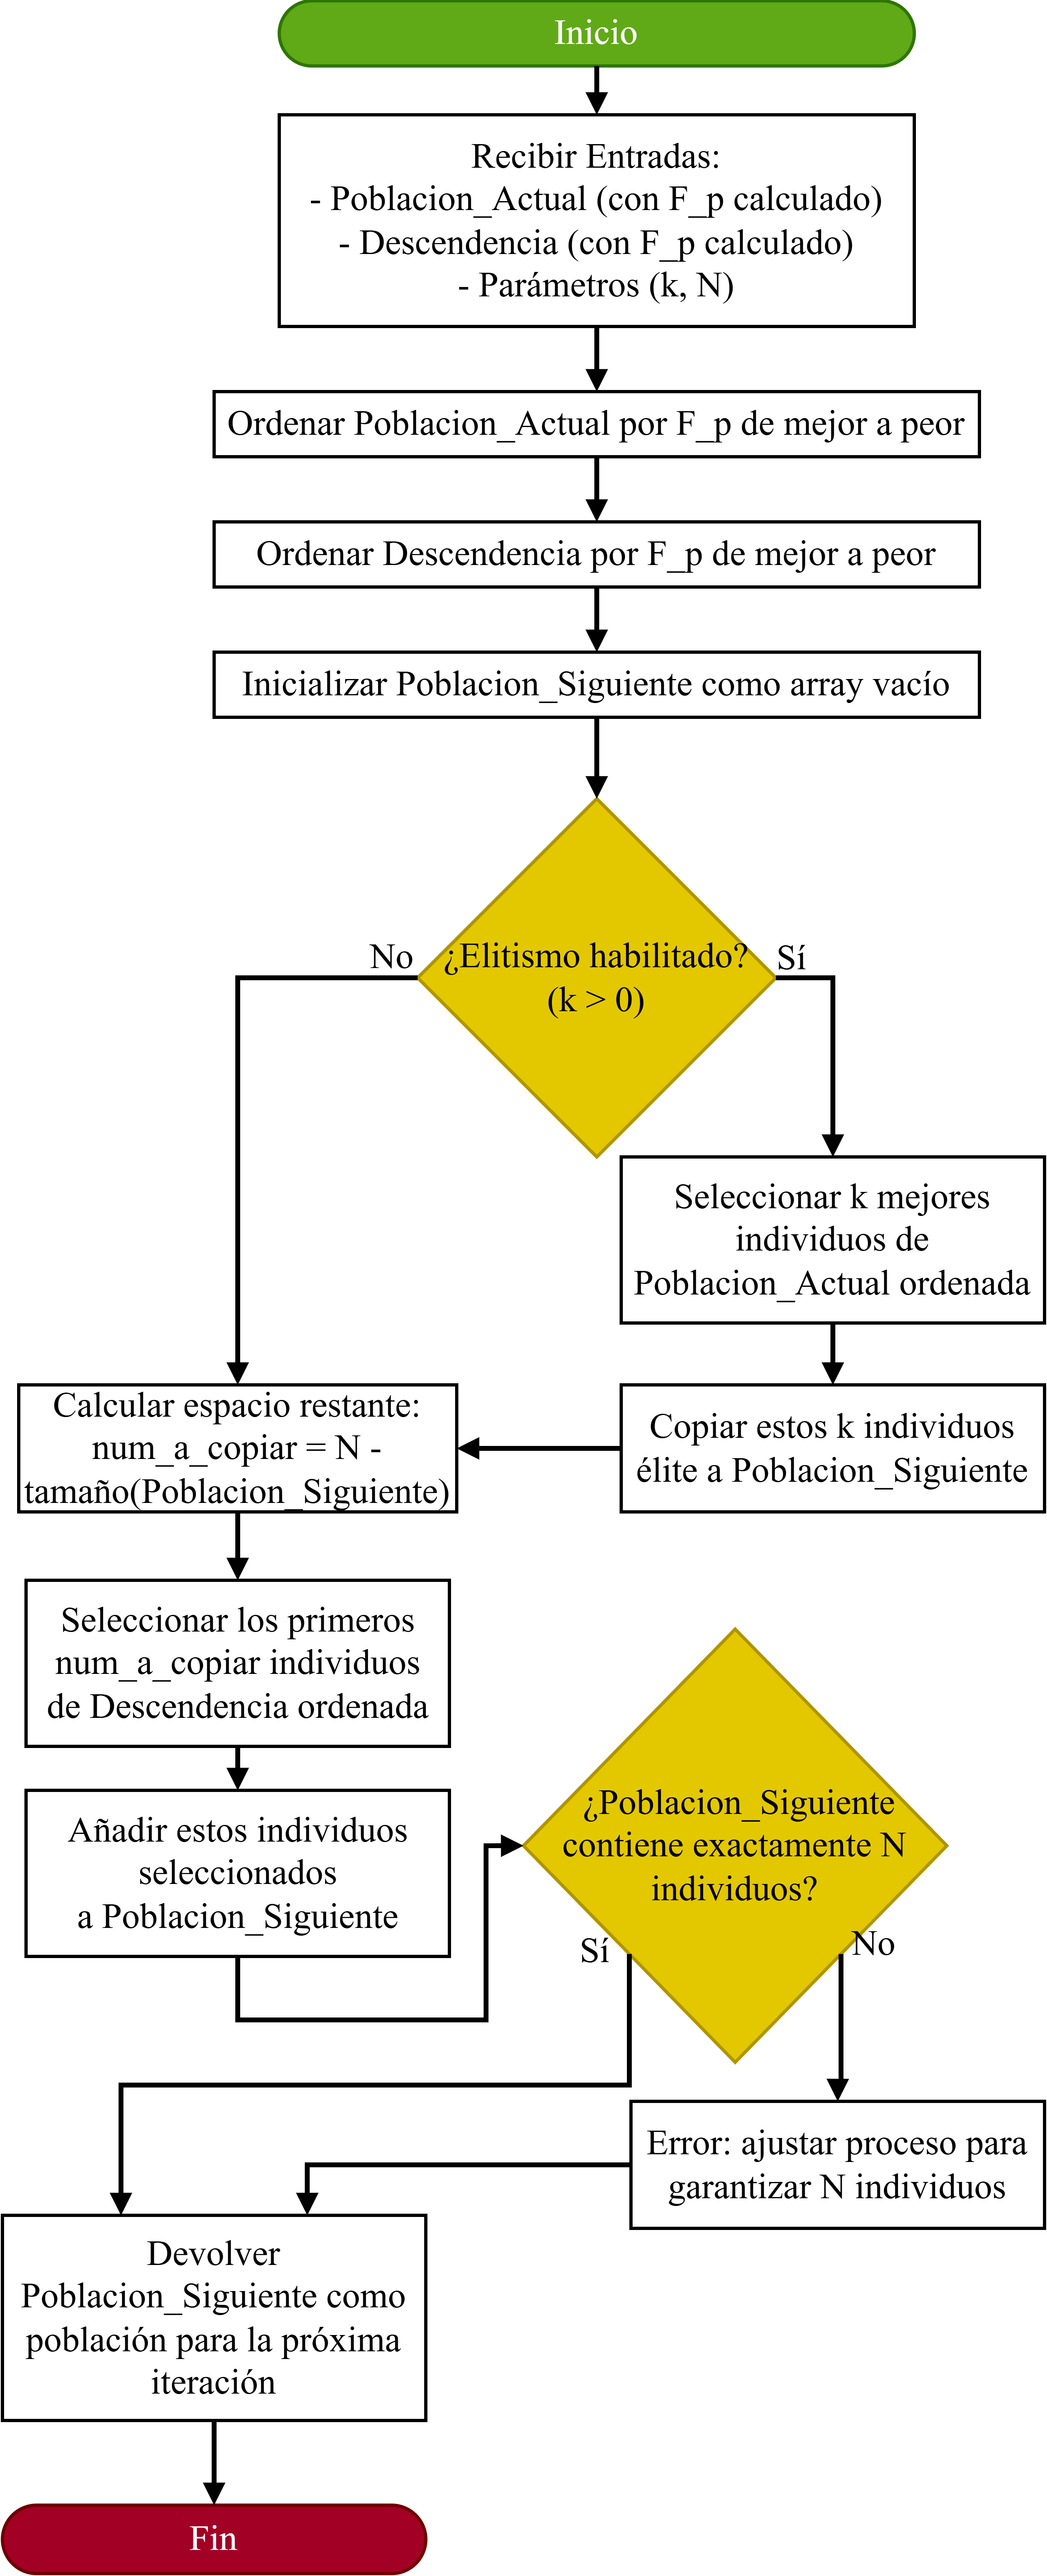
\includegraphics[width=\textwidth]{img/Analisis/DiagramaProcesos/DiagramaProceso14_SeleccionIndividuos.png}
    \caption{Diagrama de Proceso Interno 14: Selección de Individuos}%
    \label{fig:process_diagram14}
\end{figure}

\begin{figure}[H]
    \centering
    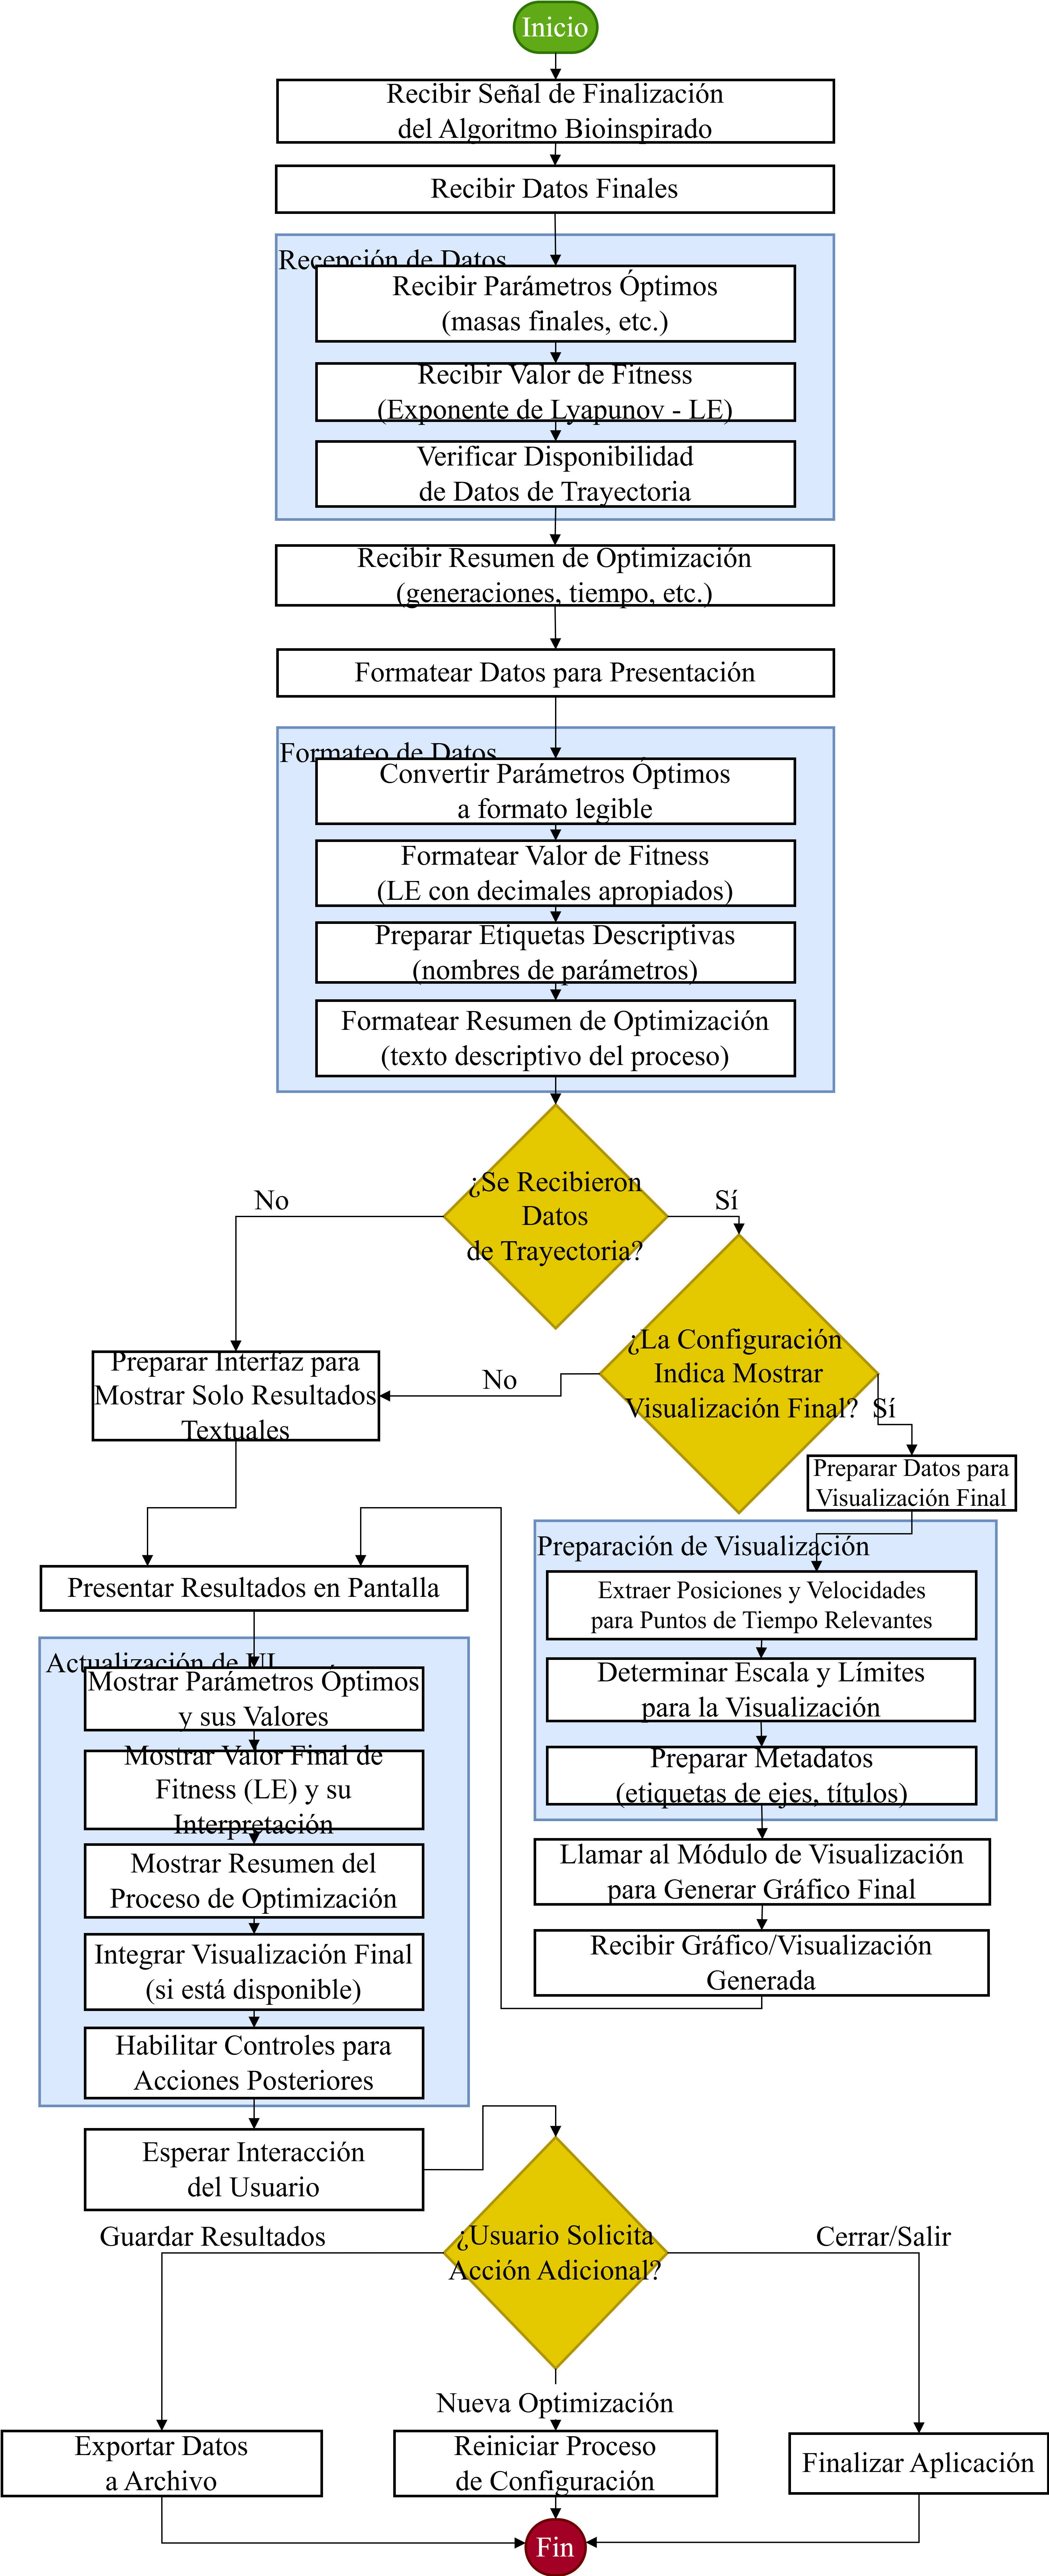
\includegraphics[width=\textwidth]{img/Analisis/DiagramaProcesos/DiagramaProceso15_Proceso Interno_Mostrar Resultados.png}
    \caption{Diagrama de Proceso Interno 15: Mostrar Resultados}%
    \label{fig:process_diagram15}
\end{figure}

    \appendix
        %\chapter{Simulator}\label{app:Simulator}
\lipsum[1]
\begin{listing}[H]
\begin{minted}[linenos, breaklines]{python}
import torch
import torch.nn as nn
import torch.nn.functional as F

class Net(nn.Module):
    def __init__(self):
        super(Net, self).__init__()
        self.conv1 = nn.Conv2d(1, 6, 5)
        self.conv2 = nn.Conv2d(6, 16, 5)
        self.fc1 = nn.Linear(16 * 5 * 5, 120)  # 5*5 from image dimension
        self.fc2 = nn.Linear(120, 84)
        self.fc3 = nn.Linear(84, 10)
    def forward(self, x):
        # ...
        return x

net = Net()
print(net)
\end{minted}
\caption{A basic neural network.}
\end{listing}
\lipsum[1]
        %\chapter{Proof of theorem}\label{app:Proof of theorem}
\lipsum[1]
\begin{figure}[thbp]
    \centering
    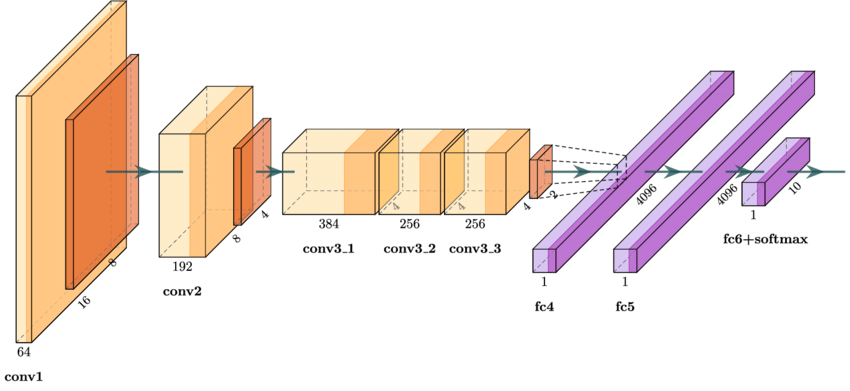
\includegraphics[width=\textwidth]{img/appendixA/alexnet.png}
    \caption{AlexNet architecture.}\label{fig:alexnet}
\end{figure}
\lipsum[1]
\begin{align}
     \vec{\nabla} \cdot \vec{E} \quad &=\quad\frac{\rho}{\epsilon_0} &&\text{Gauss's Law} \\      
    \vec{\nabla} \cdot \vec{B} \quad &=\quad 0 &&\text{Gauss's Law for Magnetism}\\
    \vec{\nabla} \times \vec{E} \quad &=\hspace{10pt}-\frac{\partial{\vec{B}}}{\partial{t}} &&\text{Faraday's Law of Induction} \\ 
    \vec{\nabla} \times \vec{B} \quad &=\quad \mu_0\left( \epsilon_0\frac{\partial{\vec{E}}}{\partial{t}}+\vec{J}\right) &&\text{Ampere's Circuital Law}
\end{align}

We can find more information in ~\cite{li2018deep}.

\backmatter%
    \bookmarksetup{startatroot}
    \printbibliography[heading=bibintoc]
\end{document}
